% SIAM Shared Information Template
% This is information that is shared between the main document and any
% supplement. If no supplement is required, then this information can
% be included directly in the main document.
The method stated above was implemented and consolidated into \RACE library. The library provides easy interface for parallelizing kernels, user typically just needs to supply the serial code (with dependency) and hardware settings. Library will then parallelize, pin and run the code in parallel. The library is publicly available in the git repository. %TODO

\subsection{Test setup}
In the following we present the performance and convergence results obtained using the library, and compare it against state of art methods. \SymmSpmv and \SYMMKACZ are chosen as representative benchmark kernels. Hardware and matrices as described in \cref{Sec:test_bed} is used for the following benchmarks. As mentioned in \cref{Sec:param_study} parameter $\epsilon_s$ is set to 0.8 and \RCM is used in level construction stage. The matrix is pre-processed with \RCM for all the cases (even for \SpMV). \SPMP \cite{SpMP} library was used to do this \RCM pre-processing.

The test setup is so constructed that it replicates the behavior of these kernels in actual practical scenarios. Normally matrix vector multiplication is followed by different calls to other kernels that use other helper data. This may lead to eviction of residual data from matrix vector multiplication. In order to replicate this behavior for \SymmSpmv and \SpMV (used as reference) we use  two ring buffers holding vectors of size \nrows. Number of vectors in this ring buffer is chosen such that these two ring buffer occupy a size of 100 \MB, which is at least two times bigger that the combined cache size of the two architectures considered. The kernels are then run two times over these ring buffer, and mean performance of the runs is taken into account.

For \SYMMKACZ there are two use cases. In one it is used as a plain iterative solver where the kernel is called successively. The other use case of this iterative solver is in algorithms like CGMN~\cite{CGMN, CGMN_gordon} or CARP-CG~\cite{CARP-CG} where \SYMMKACZ is used like a preconditioner, where an approach similar to \SymmSpmv have to be used for benchmarking. In this paper the benchmark is constructed to replicate the behavior of the former case, \ie we call the \SYMMKACZ kernel 500 times in succession and report the mean performance. It has to be noted that the difference in performance measurements between these two benchmarks is very small and only affects small matrices.


\subsection{Corner Cases}



\Cref{fig:corner_cases_scaling} shows the scaling performance of \SymmSpmv and \SpMV (baseline) kernel for corner case matrices on one socket of \SKX architecture. Chosen corner case matrices represent different aspects and bottlenecks that appear either due to \RACE method or because of hardware capabilities.

 The \emph{crankseg\_1} matrix is the worst in terms of performance. It does not scale well due to it's limited parallelism obtained using the \RACE method. This property of \emph{crankseg\_1} is well evident directly after doing the theoretical estimate based on $\eta$ as  seen in \cref{fig:crankseg_param}. One could further see that the actual scaling run of the kernel seen in \cref{fig:crankseg_scaling} is exactly in tune with that of the theoretical result. Note that due to this bottleneck of parallelism we didn't achieve much benefit from using \SymmSpmv compared to \SpMV.

The \emph{inline\_1} matrix although being third lowest in terms of parallelism in the entire set of test matrices, but it still achieves a high efficiency ($\eta$ = 0.85) for 20 threads (see \cref{fig:inline_param}), leading to good scaling as seen in \cref{fig:inline_scaling}. The saturation in performance after 15 threads is due to the fact that we hit the memory bottleneck, similar saturation behavior can also be observed for \SpMV which is embarrassingly parallel. The saturation occurs at the maximum achievable performance on the given architecture which could easily be verified using the \roofline model \cite{Williams_roofline} and intensity equations (see \cref{subsec:test_kernels}) as shown below:
\begin{align*}
	% P_{max} =&  2 \fracUnit{FMA AVX-512 instruction}{cy*cores}  * 8 \fracUnit{FMA}{FMA AVX-512 instruction} \\
	% & * 2 \fracUnit{Flop}{FMA} * 2.4 \fracUnit{Gcy}{s} * 20 \unit{cores} = 1536  \fracUnit{GFlop}{s} \\	 
	 I_\mathrm{\SpMV} &= \frac{2}{8+4+\frac{8+16}{73}} = 0.162 \fracUnit{Flop}{byte} \text{, assuming best case : $\alpha = \frac{1}{\NNZRmath}$}\\
	 P_\mathrm{\SpMV} &= b_s*I_\mathrm{\SpMV}; \text{  for memory-bound case}\\
	 P_\mathrm{\SpMV} &= 0.162\fracUnit{Flop}{Bytes}*115\fracUnit{GByte}{s} = 18.6 \fracUnit{GFlop}{s}\\
\end{align*}

As seen we achieve 17.8 GFlop/s which is close to the theoretical maximum of 18.6 GFlop/s for \SpMV. Similar derivation can be done for \SymmSpmv and one could see $P_\mathrm{\SymmSpmv}$= 34.5 GFlop/s, which is approximately twice that of \SpMV since $I_\mathrm{\SymmSpmv}$ is almost a factor two higher than $I_\mathrm{\SpMV}$ for matrix with moderate \NNZR (see \cref{eq:SpMV_intensity,eq:SymmSpMV_intensity}). From \cref{fig:inline_scaling} one can observe that at saturation we reach close to theoretical values. A cushioning effect due to memory bandwidth bottleneck is also evident from \cref{fig:inline_scaling}, where we see that due to this saturation decrease in $\eta$ to a certain extent would not effect the socket level performance, it would just shift the knee of saturation towards right.

In the case of \emph{parabolic\_fem} matrix we theoretically have a good efficiency as seen from \cref{fig:parabolic_fem_param}, but here we do not see any saturation in performance (see \cref{fig:parabolic_fem_scaling}), even \SpMV does not have this saturation behavior. If one calculates the maximum  theoretical performance by \roofline model and assuming memory-boundedness as shown in previous example one would see that $P_\mathrm{\SpMV}$=15 GFlop/s and $P_\mathrm{\SymmSpmv}$=19 GFlop/s, but we achieve more than these values in actual runs 26.5 and 31.5 GFlop/s respectively. This is because the matrix is small enough ($\approx$ 46 MB for full matrix and $\approx$ 23 MB for symmetric storage) to just fit in caches (combined L2 and L3) of the \SKX architecture. Since the caches scales well on this architecture we don't observe the saturation behavior. It should be noted that in this case comparison between \SpMV and \SymmSpmv cannot be done directly since for \SpMV the total data is almost close to cache limits, while for \SymmSpmv it would easily fit in cache.

\emph{Graphene-4096} matrix on the other hand is a matrix with efficiency similar to \emph{parabolic\_fem} but with much larger size ($\approx 2 GB$) resulting in matrix data always coming from main memory. This therefore shows dominant saturation behavior and since we achieve good efficiency ($\eta$) the knee of saturation begins at a well early stage for \SymmSpmv compared to  the case of \emph{inline\_1} where the efficiency was lower in comparison resulting in smaller \threadEff.

\subsection{Performance and comparisons}

\begin{figure}[thbp]
	\centering
	\subfloat[Comparison of \SpMV and RACE \SymmSpmv on 1 socket of \IVB]{\label{fig:spmv_vs_symm_spmv_ivy}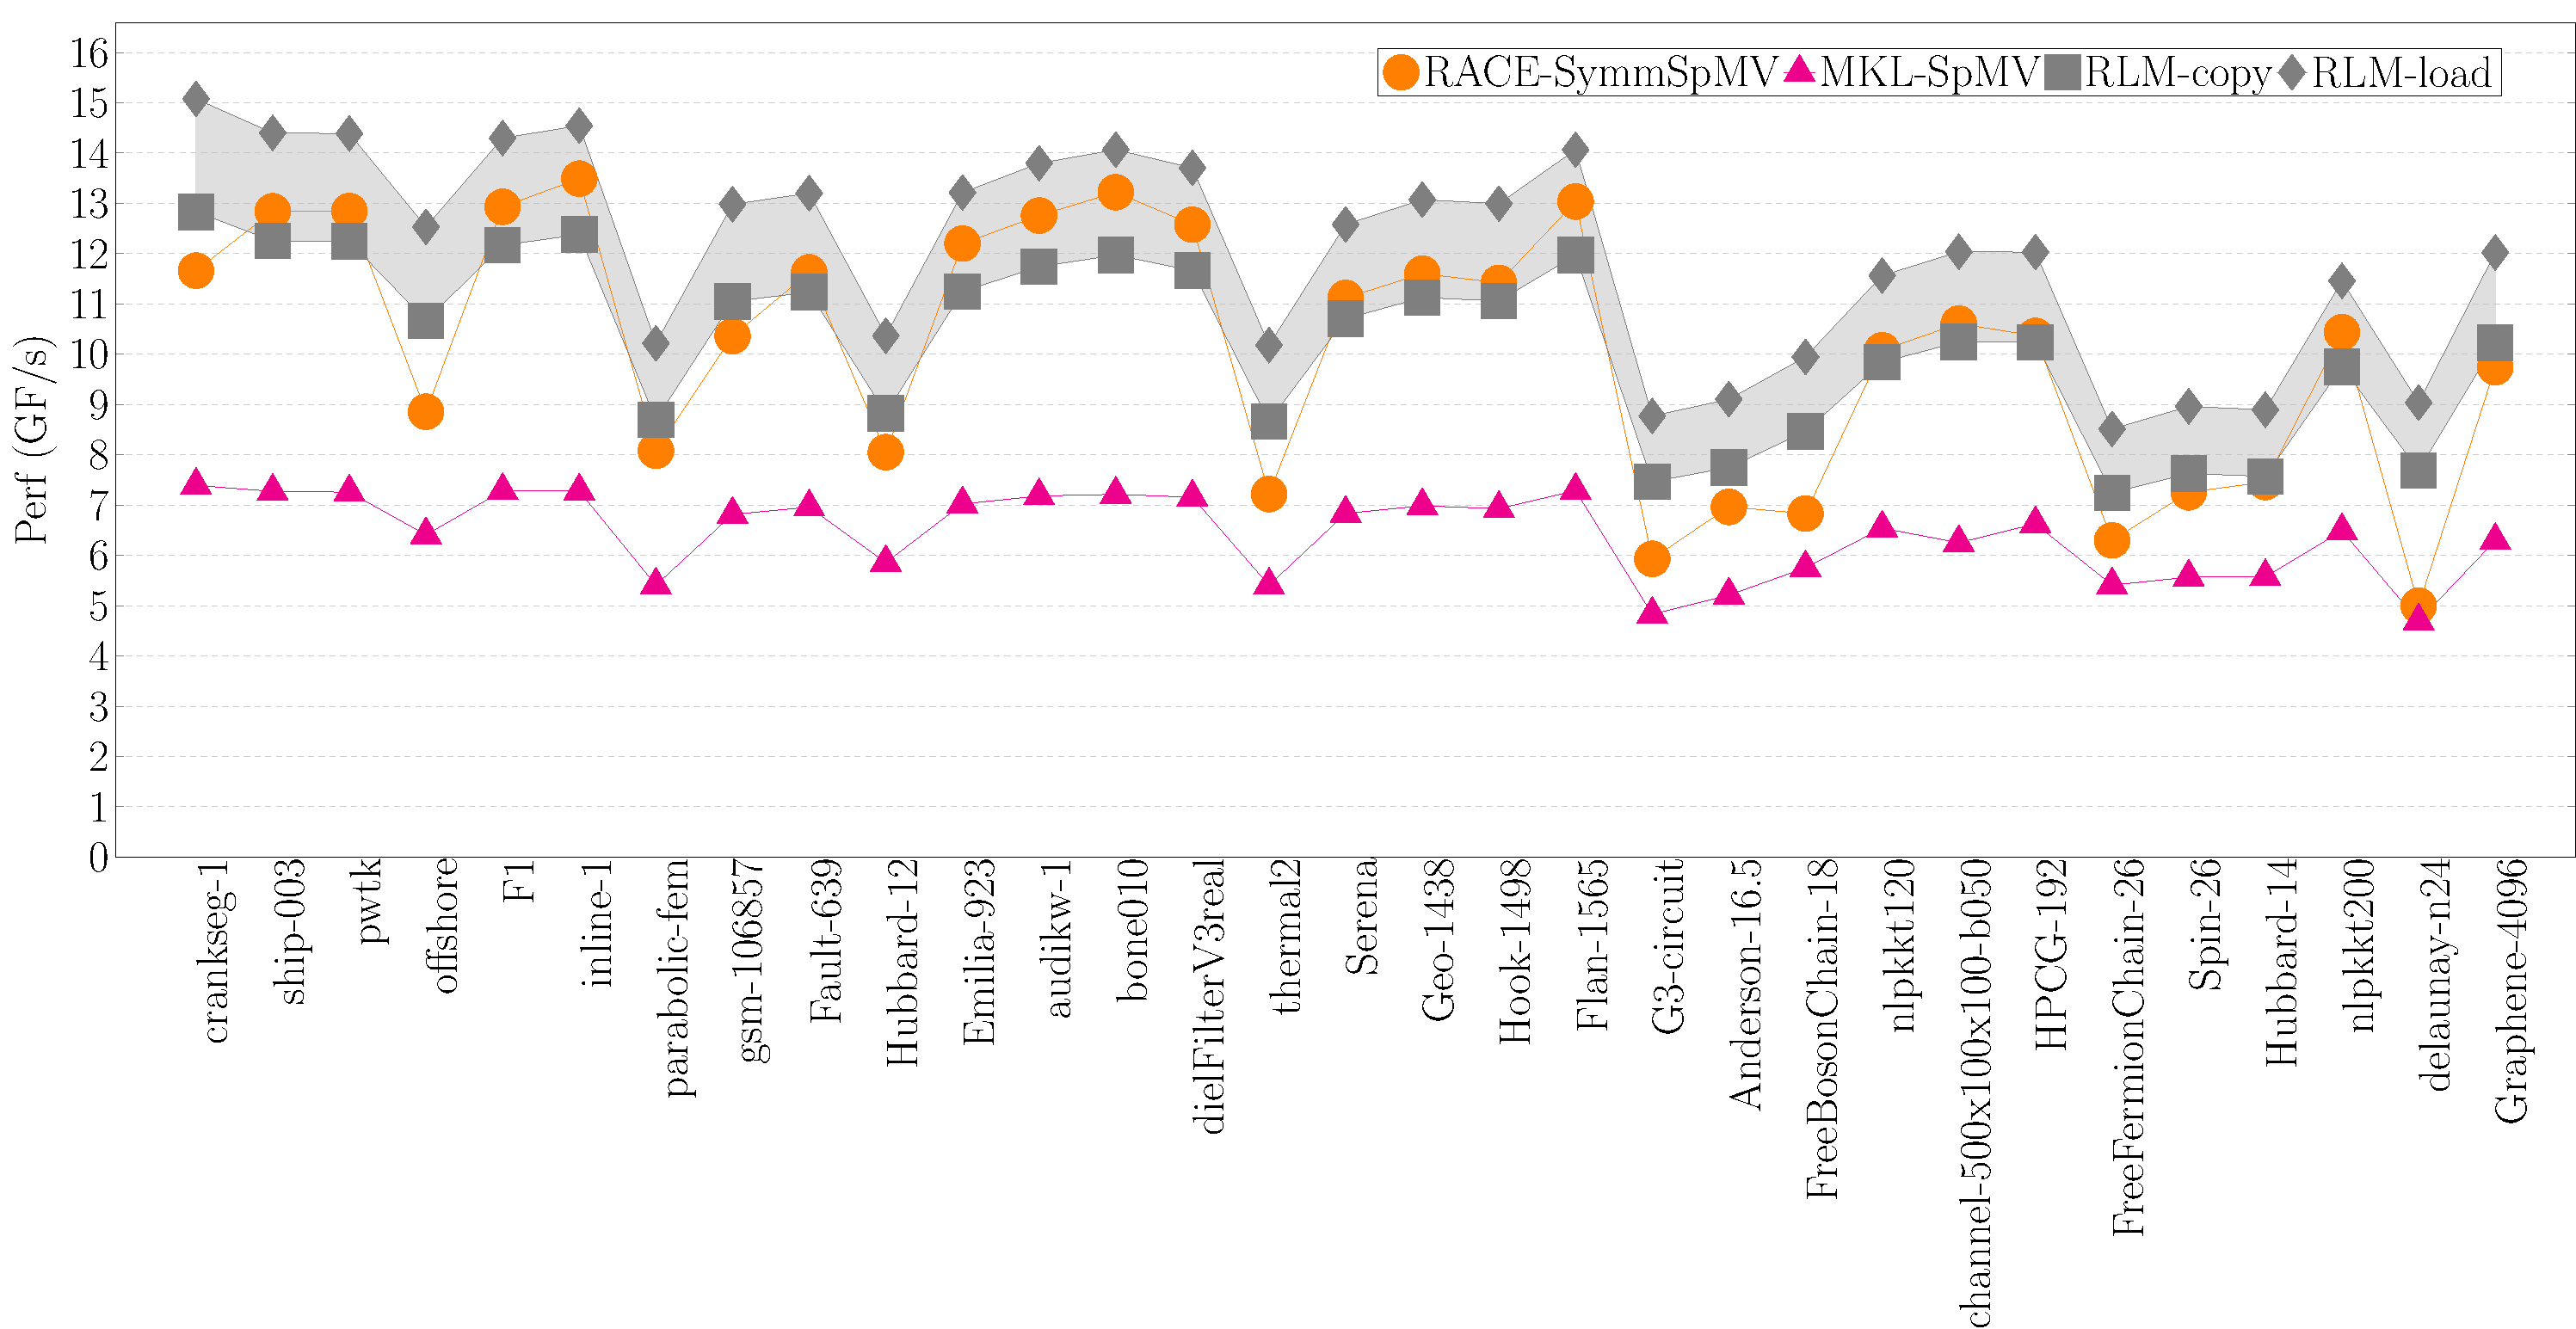
\includegraphics[width=0.85\textwidth, height=0.27\textheight]{pics/results/ivy/data_symm_spmv/plot_generator/perf_vs_mtx_RACE_w_SpMV/perf}}
	\hspace{1em}
	\subfloat[\SymmSpmv on 1 socket of \SKX]{\label{fig:spmv_vs_symm_spmv_skx}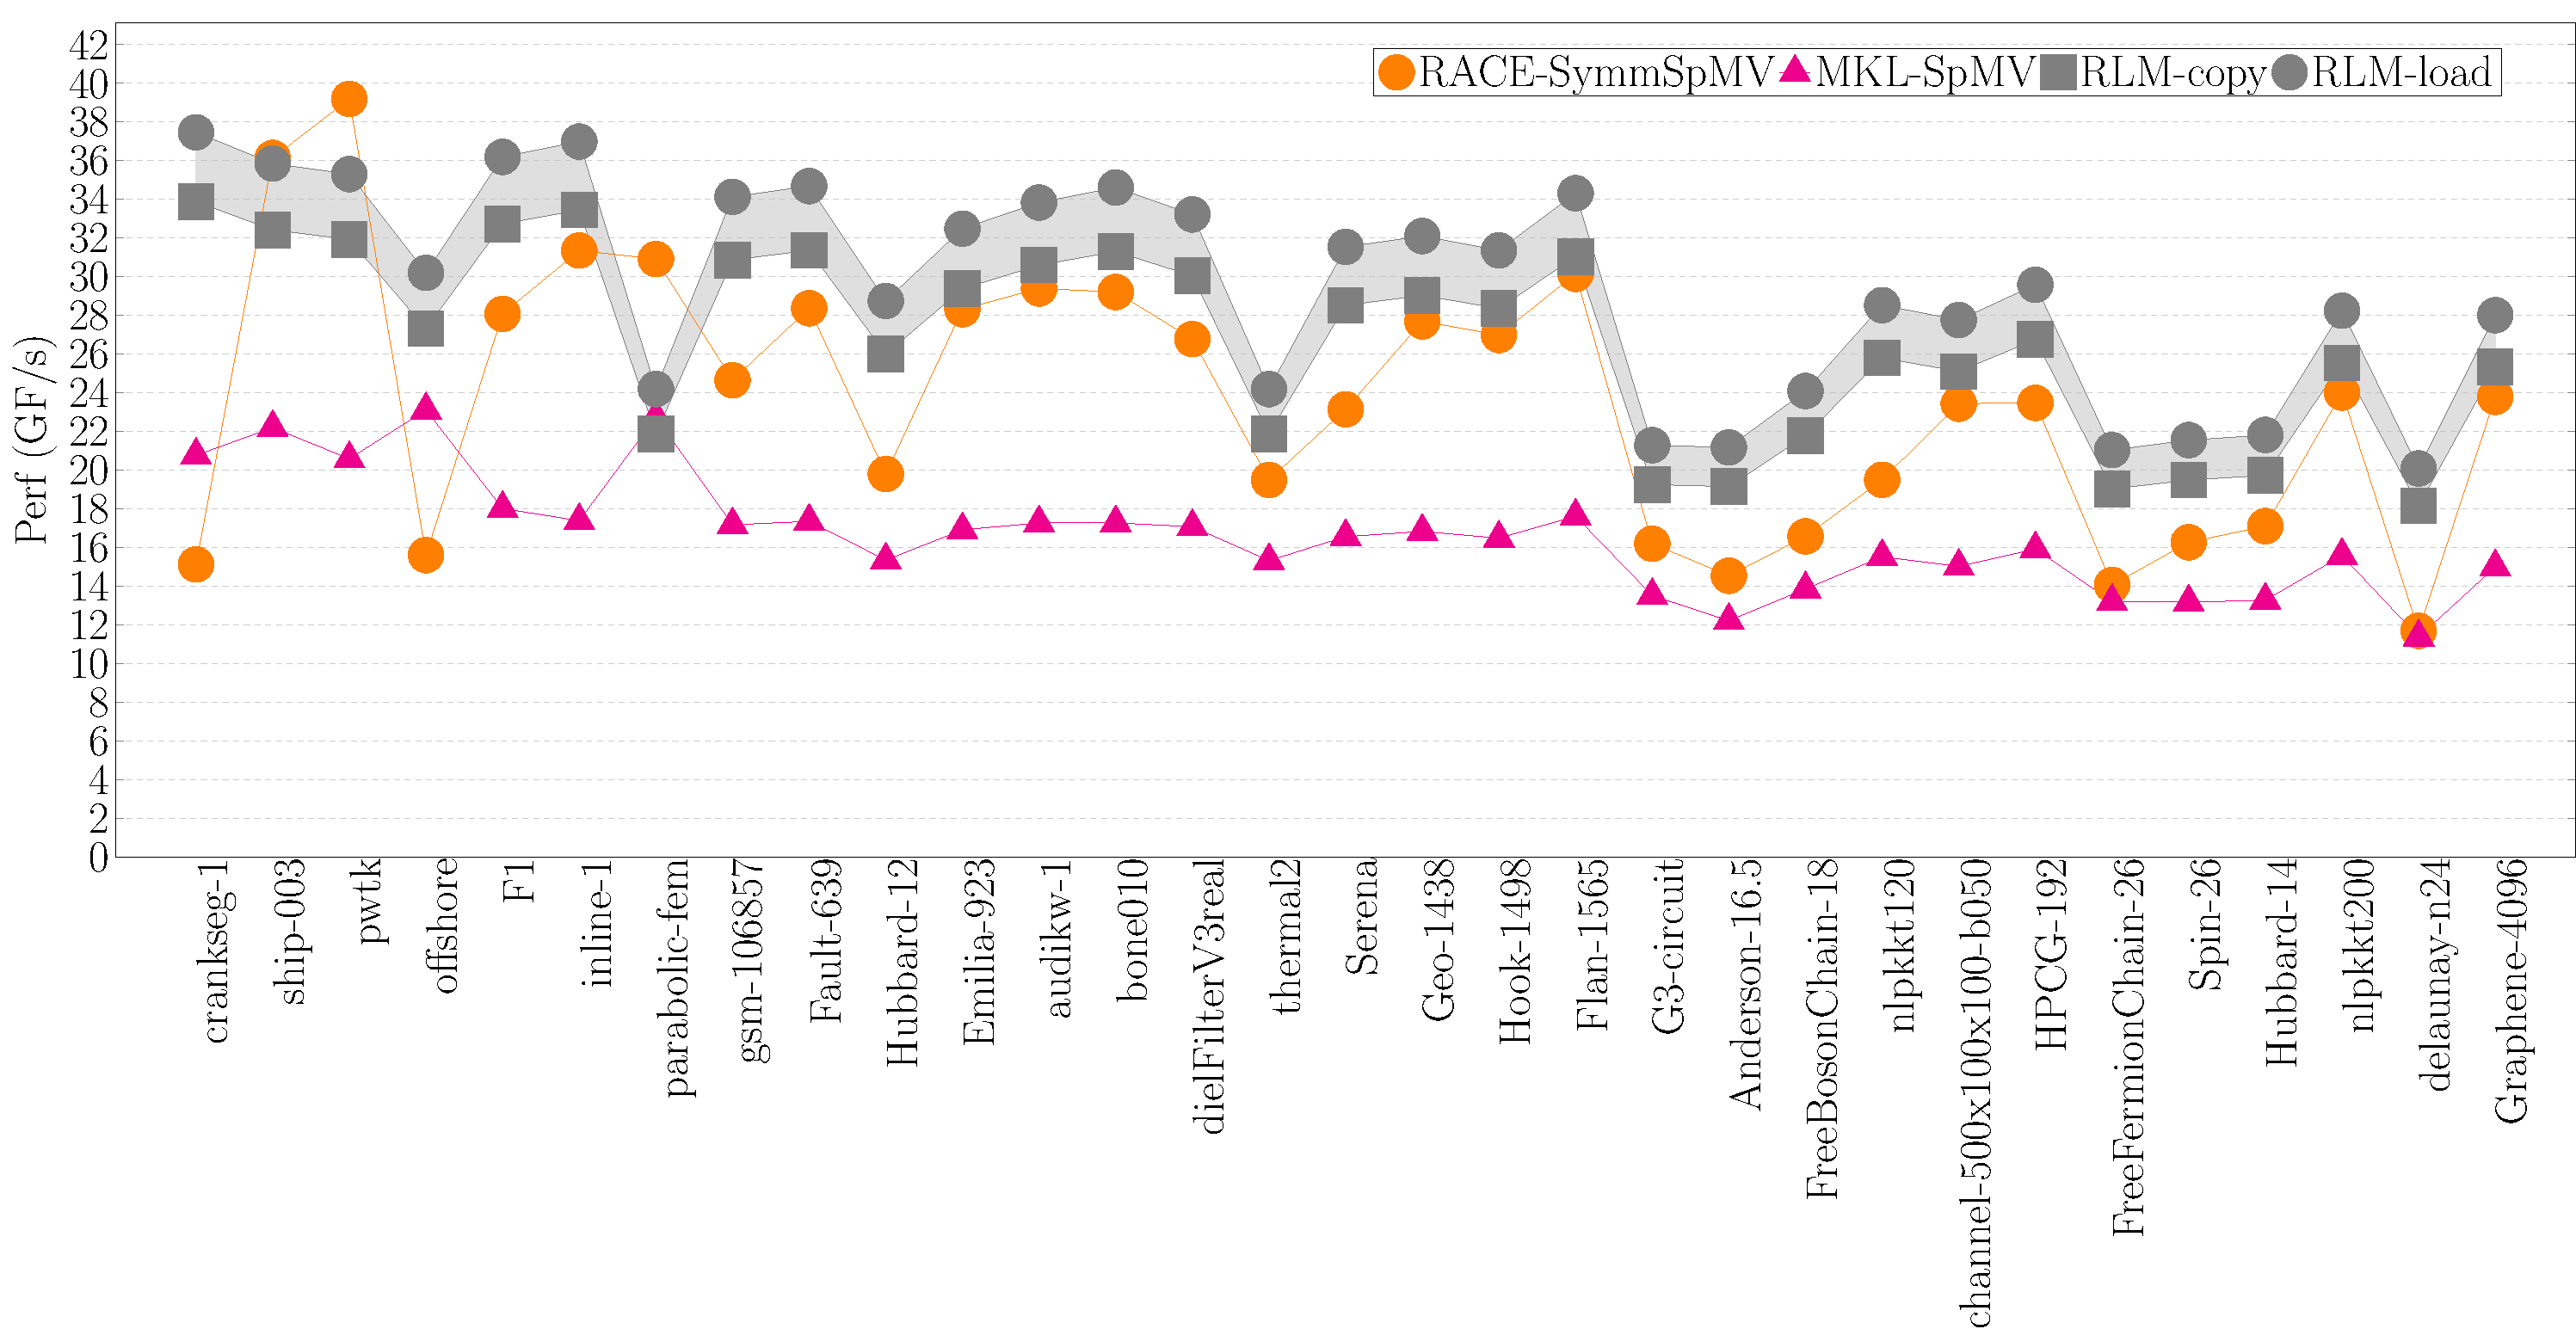
\includegraphics[width=0.85\textwidth, height=0.27\textheight]{pics/results/skx/data_symm_spmv/plot_generator/perf_vs_mtx_RACE_w_SpMV/perf}}
	\caption{\SpMV vs RACE \SymmSpmv performance}
	\label{fig:SpMV_vs_SymmSpMV}
\end{figure}
\subsection{RACE performance in comparison to SpMV}
\begin{table}[ht]
	\footnotesize
	\caption{$\alpha$ values of SpMV measured using \LIKWID for both architectures }
	\label{table:alpha_values}
	\begin{center}
		\begin{tabular}{|l|l|S[round-mode=places,round-precision=4]|S[round-mode=places,round-precision=4]|S[round-mode=places,round-precision=4]|S[round-mode=places,round-precision=4]|}
\toprule
\multirow{2}{*}{Index} & \multirow{2}{*}{Matrix name} & \multicolumn{3}{c|}{$\alpha_{SpMV}$} & {$I_{\acrshort{SpMV}}(\alpha_{SpMV})$} \\
%\midrule
\cline{3-6}
& &  {optimal} & {SKX} & {IVB} & {optimal}  \\
\midrule
{1}& {	crankseg\_1                }	& 0.004974840341951422	& 0.009900427637091272*	& 0.017876	& 0.16475420629866486	\\
{2}& {	ship\_003                  }	& 0.015054104375856307	& 0.029661678743938248*	& 0.039038	& 0.16101095659221026	\\
{3}& {	pwtk                      }	& 0.018730450092715727	& 0.03677214142565592*	& 0.038276	& 0.1596876177714501	\\
{4}& {	offshore                  }	& 0.061232390023872055	& 0.11539864519682566*	& 0.105831	& 0.14583098113326293	\\
{5}& {	F1                        }	& 0.012810282496064584	& 0.025296509558520128*	& 0.043622	& 0.16182947693011468	\\
{6}& {	inline\_1                  }	& 0.013681750417974054	& 0.013709	& 0.034046	& 0.16151058900649082	\\
{7}& {	parabolic\_fem             }	& 0.14309623622555628	& 0.25036603514337963*	& 0.224973	& 0.12494772020022805	\\
{8}& {	gsm\_106857                }	& 0.02708985058701268	& 0.052750692788036055*	& 0.094584	& 0.15675804527541276	\\
{9}& {	Fault\_639                 }	& 0.022324366119157866	& 0.045281	& 0.086085	& 0.15841480951843234	\\
{10}& {	Hubbard-12                }	& 0.07692947982285911	& 0.14286818452683273*	& 0.231786	& 0.14130255800224512	\\
{11}& {	Emilia\_923                }	& 0.022512653462004855	& 0.08265	& 0.085462	& 0.15834868547473438	\\
{12}& {	audikw\_1                  }	& 0.012152898336217176	& 0.062422	& 0.063762	& 0.16207086168751325	\\
{13}& {	bone010                   }	& 0.013768014517655372	& 0.049208	& 0.052338	& 0.16147909155409917	\\
{14}& {	dielFilterV3real          }	& 0.01234882033880347	& 0.072827	& 0.067509	& 0.16199884583462107	\\
{15}& {	thermal2                  }	& 0.14312355713563962	& 0.2504078517886007*	& 0.227709	& 0.12494174903463444	\\
{16}& {	Serena                    }	& 0.02156070528689192	& 0.100582	& 0.115621	& 0.15868356434880437	\\
{17}& {	Geo\_1438                  }	& 0.022768134283905977	& 0.089589	& 0.091725	& 0.15825905217944752	\\
{18}& {	Hook\_1498                 }	& 0.024591034497360605	& 0.103075	& 0.094818	& 0.1576224362116434	\\
{19}& {	Flan\_1565                 }	& 0.013328053114104274	& 0.054135	& 0.052516	& 0.161639862432339	\\
{20}& {	G3\_circuit                }	& 0.20695912474502637	& 0.34294305499160477*	& 0.335974	& 0.11239203379889182	\\
{21}& {	Anderson-16.5             }	& 0.14285714285714285	& 0.363368	& 0.318715	& 0.125	\\
{22}& {	FreeBosonChain-18         }	& 0.08024691655235494	& 0.27076	& 0.262774	& 0.14038128167567254	\\
{23}& {	nlpkkt120                 }	& 0.03657773850304069	& 0.160002	& 0.165642	& 0.15356057042478993	\\
{24}& {	channel-500x100x100-b050  }	& 0.05325806761196896	& 0.173504	& 0.133898	& 0.14824449726378677	\\
{25}& {	HPCG-192                  }	& 0.03742553488106633	& 0.135801	& 0.139089	& 0.15328119500901655	\\
{26}& {	FreeFermionChain-26       }	& 0.07396449704142012	& 0.387859	& 0.397282	& 0.1421362489486964	\\
{27}& {	Spin-26                   }	& 0.07142857142857142	& 0.367034	& 0.351781	& 0.14285714285714285	\\
{28}& {	Hubbard-14                }	& 0.06666796002509115	& 0.357508	& 0.359807	& 0.14423039256024434	\\
{29}& {	nlpkkt200                 }	& 0.036231752783504406	& 0.16692	& 0.172028	& 0.15367487636455557	\\
{30}& {	delaunay\_n24              }	& 0.1666668333335	& 0.406459	& 0.319197	& 0.1199999663999758	\\
{31}& {	Graphene-4096             }	& 0.0769548711240621	& 0.160392	& 0.127774	& 0.14129546073388705	\\
%#TABLE_DATA#
\bottomrule
\end{tabular}



	\end{center}
\end{table}

\Cref{fig:SpMV_vs_SymmSpMV} provides performance of SymmSpMV compared to SpMV. Roofline \cite{Williams_roofline} model for each of the matrices is also shown in the figure. The model takes into account the alpha factor, which is derived based on SpMV performance.

 From the figure one can observe that in some cases roofline performance is lower than that of actual measured performance. This is due to the fact that these are small matrices and some of the data can fit in the cache, since \SKX has cumulatively larger cache compared to \IVB we observe more matrices showing this kind of behavior.
 
 The figure also makes it clear that eventhough we only operate with upper triangle part of the matrix, it is not always the case we get a factor of two in performance. There are basically two reasons for it as suggested by roofline model:
 \begin{enumerate}
 	\item Small non-zeros per row \NNZR: If \NNZR its symmetric variant \NNZRSYMM will be even smaller, since this term enters into denominator of $I_{\SymmSpmv}$ as shown in \cref{eq:SymmSpMV_intensity} it decreases the performance even more.
 	\item $\alpha$ factor: The effect of $\alpha$ on \SymmSpmv kernel is more than that of \SpMV. One can observe this by comparing \cref{eq:SpMV_intensity,eq:SymmSpMV_intensity}, where the  pre-factor of $\alpha$ is three times bigger for \SymmSpmv.
 \end{enumerate}

\begin{figure}[thbp]
	\centering
	\subfloat[\SymmSpmv on 1 socket of \IVB]{\label{fig:symm_spmv_ivy}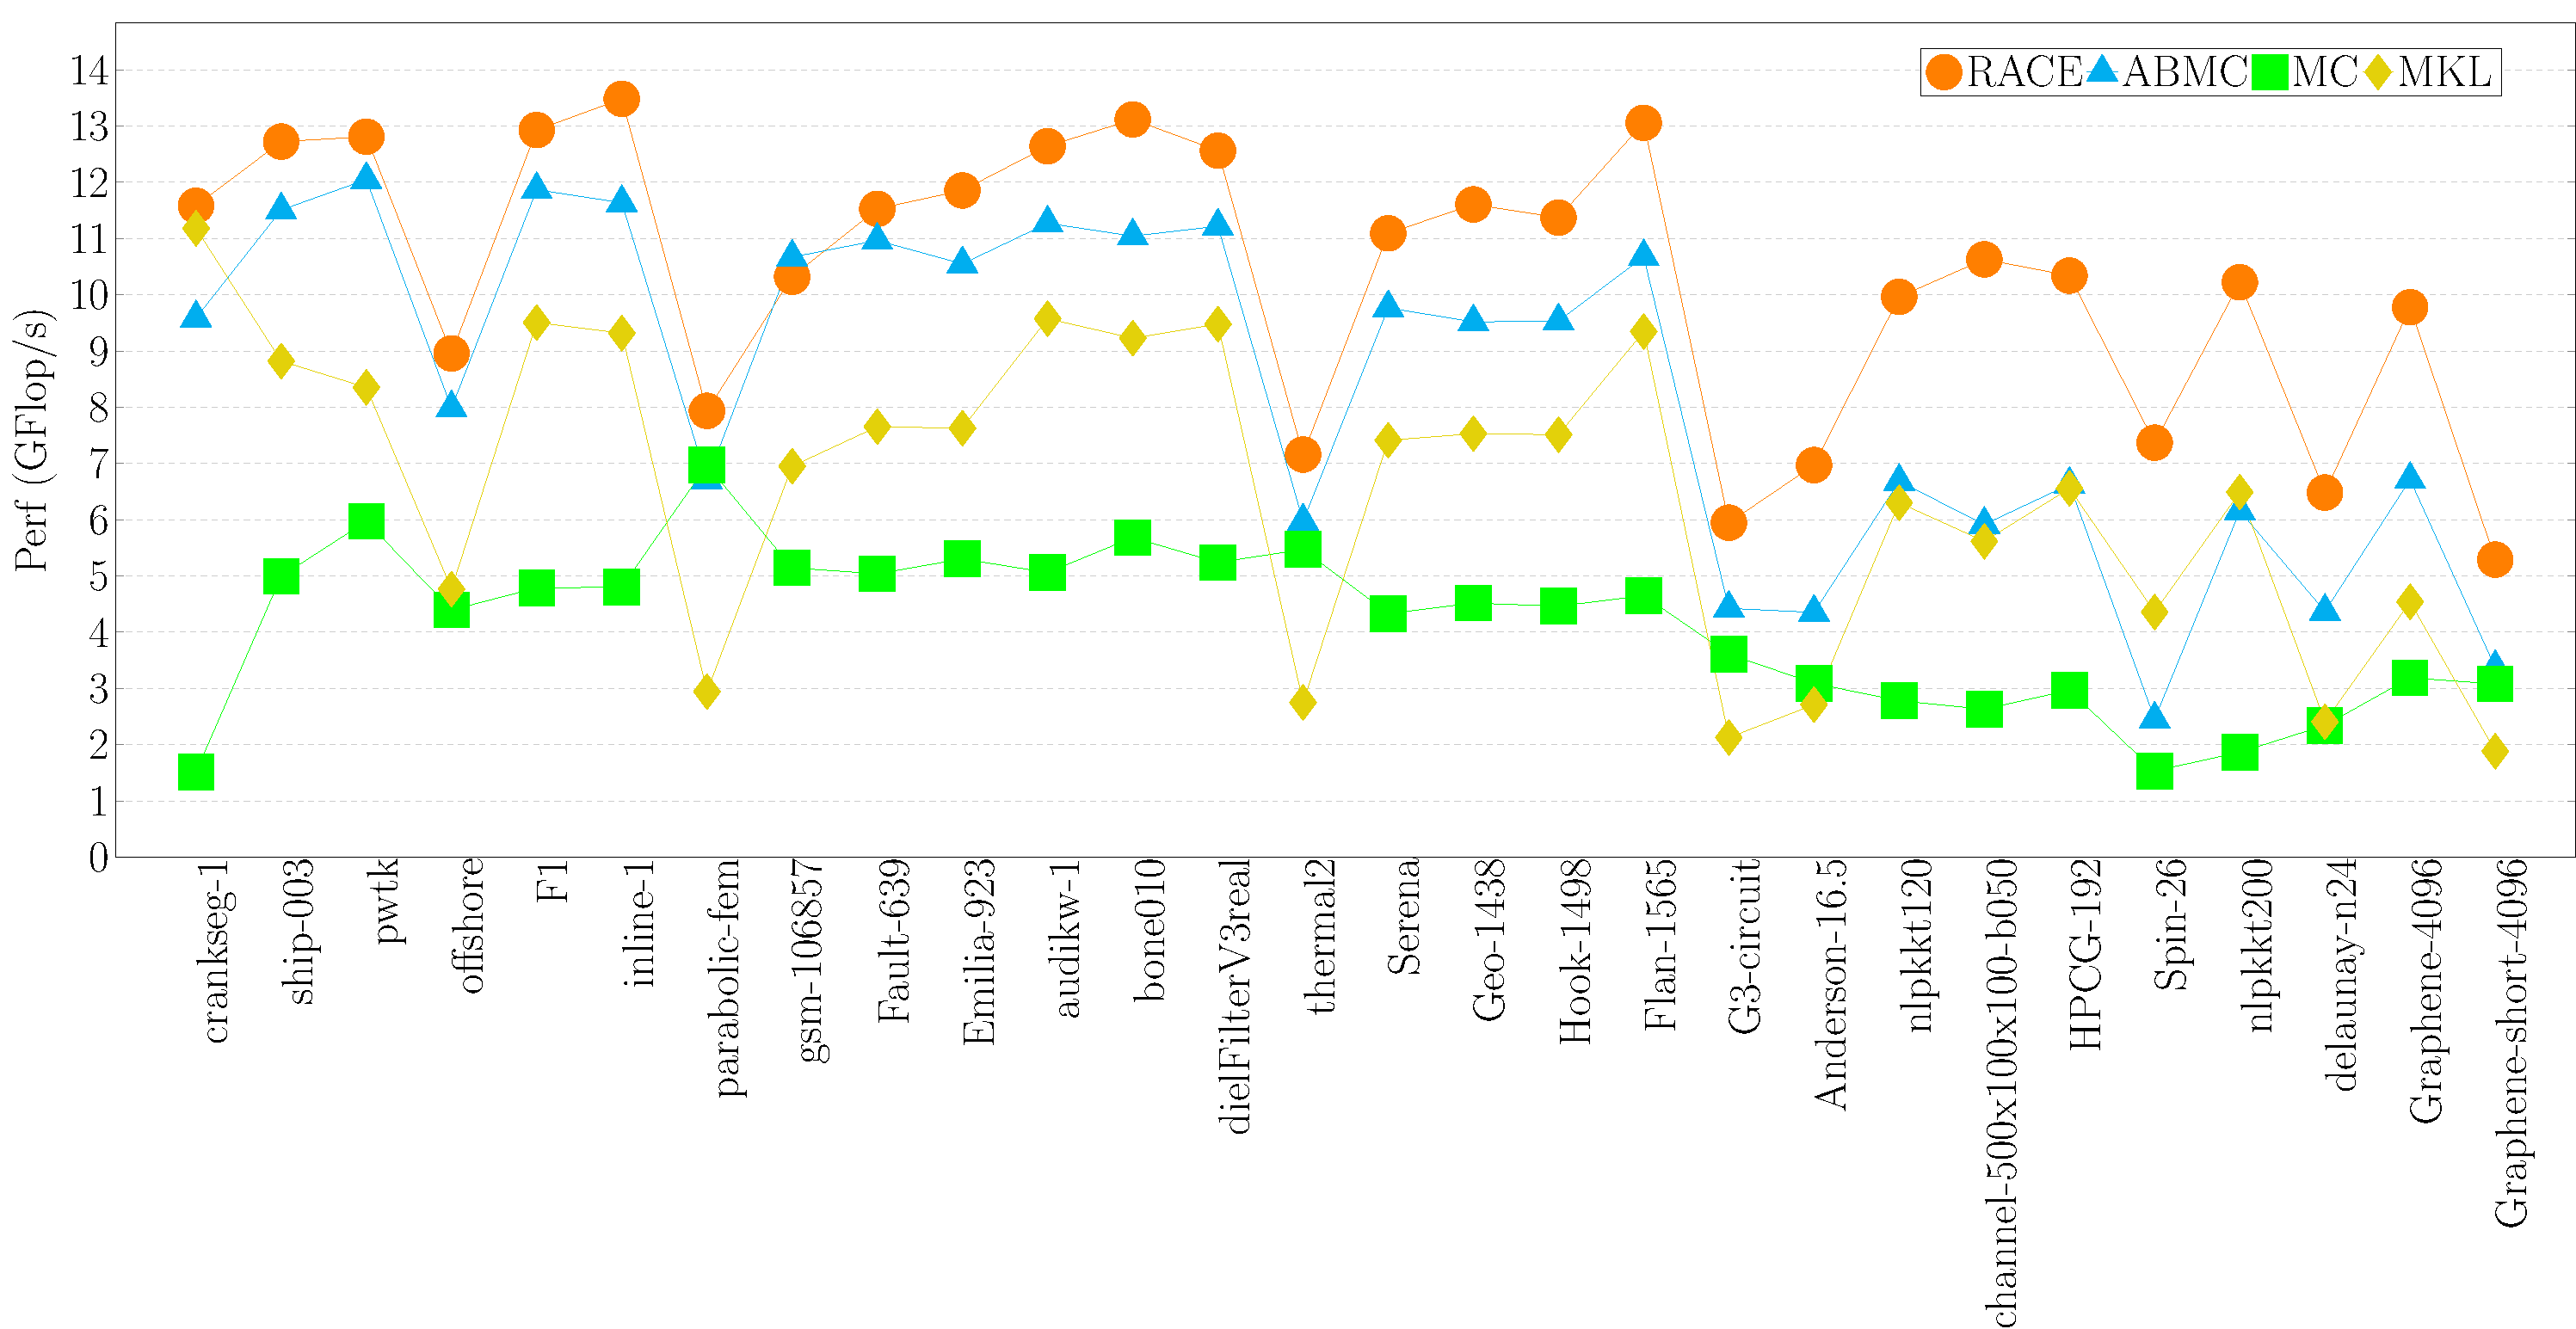
\includegraphics[width=0.85\textwidth, height=0.27\textheight]{pics/results/ivy/data_symm_spmv/plot_generator/perf_vs_mtx/perf}}
	\hspace{1em}
	\subfloat[\SymmSpmv on 1 socket of \SKX]{\label{fig:symm_spmv_skx}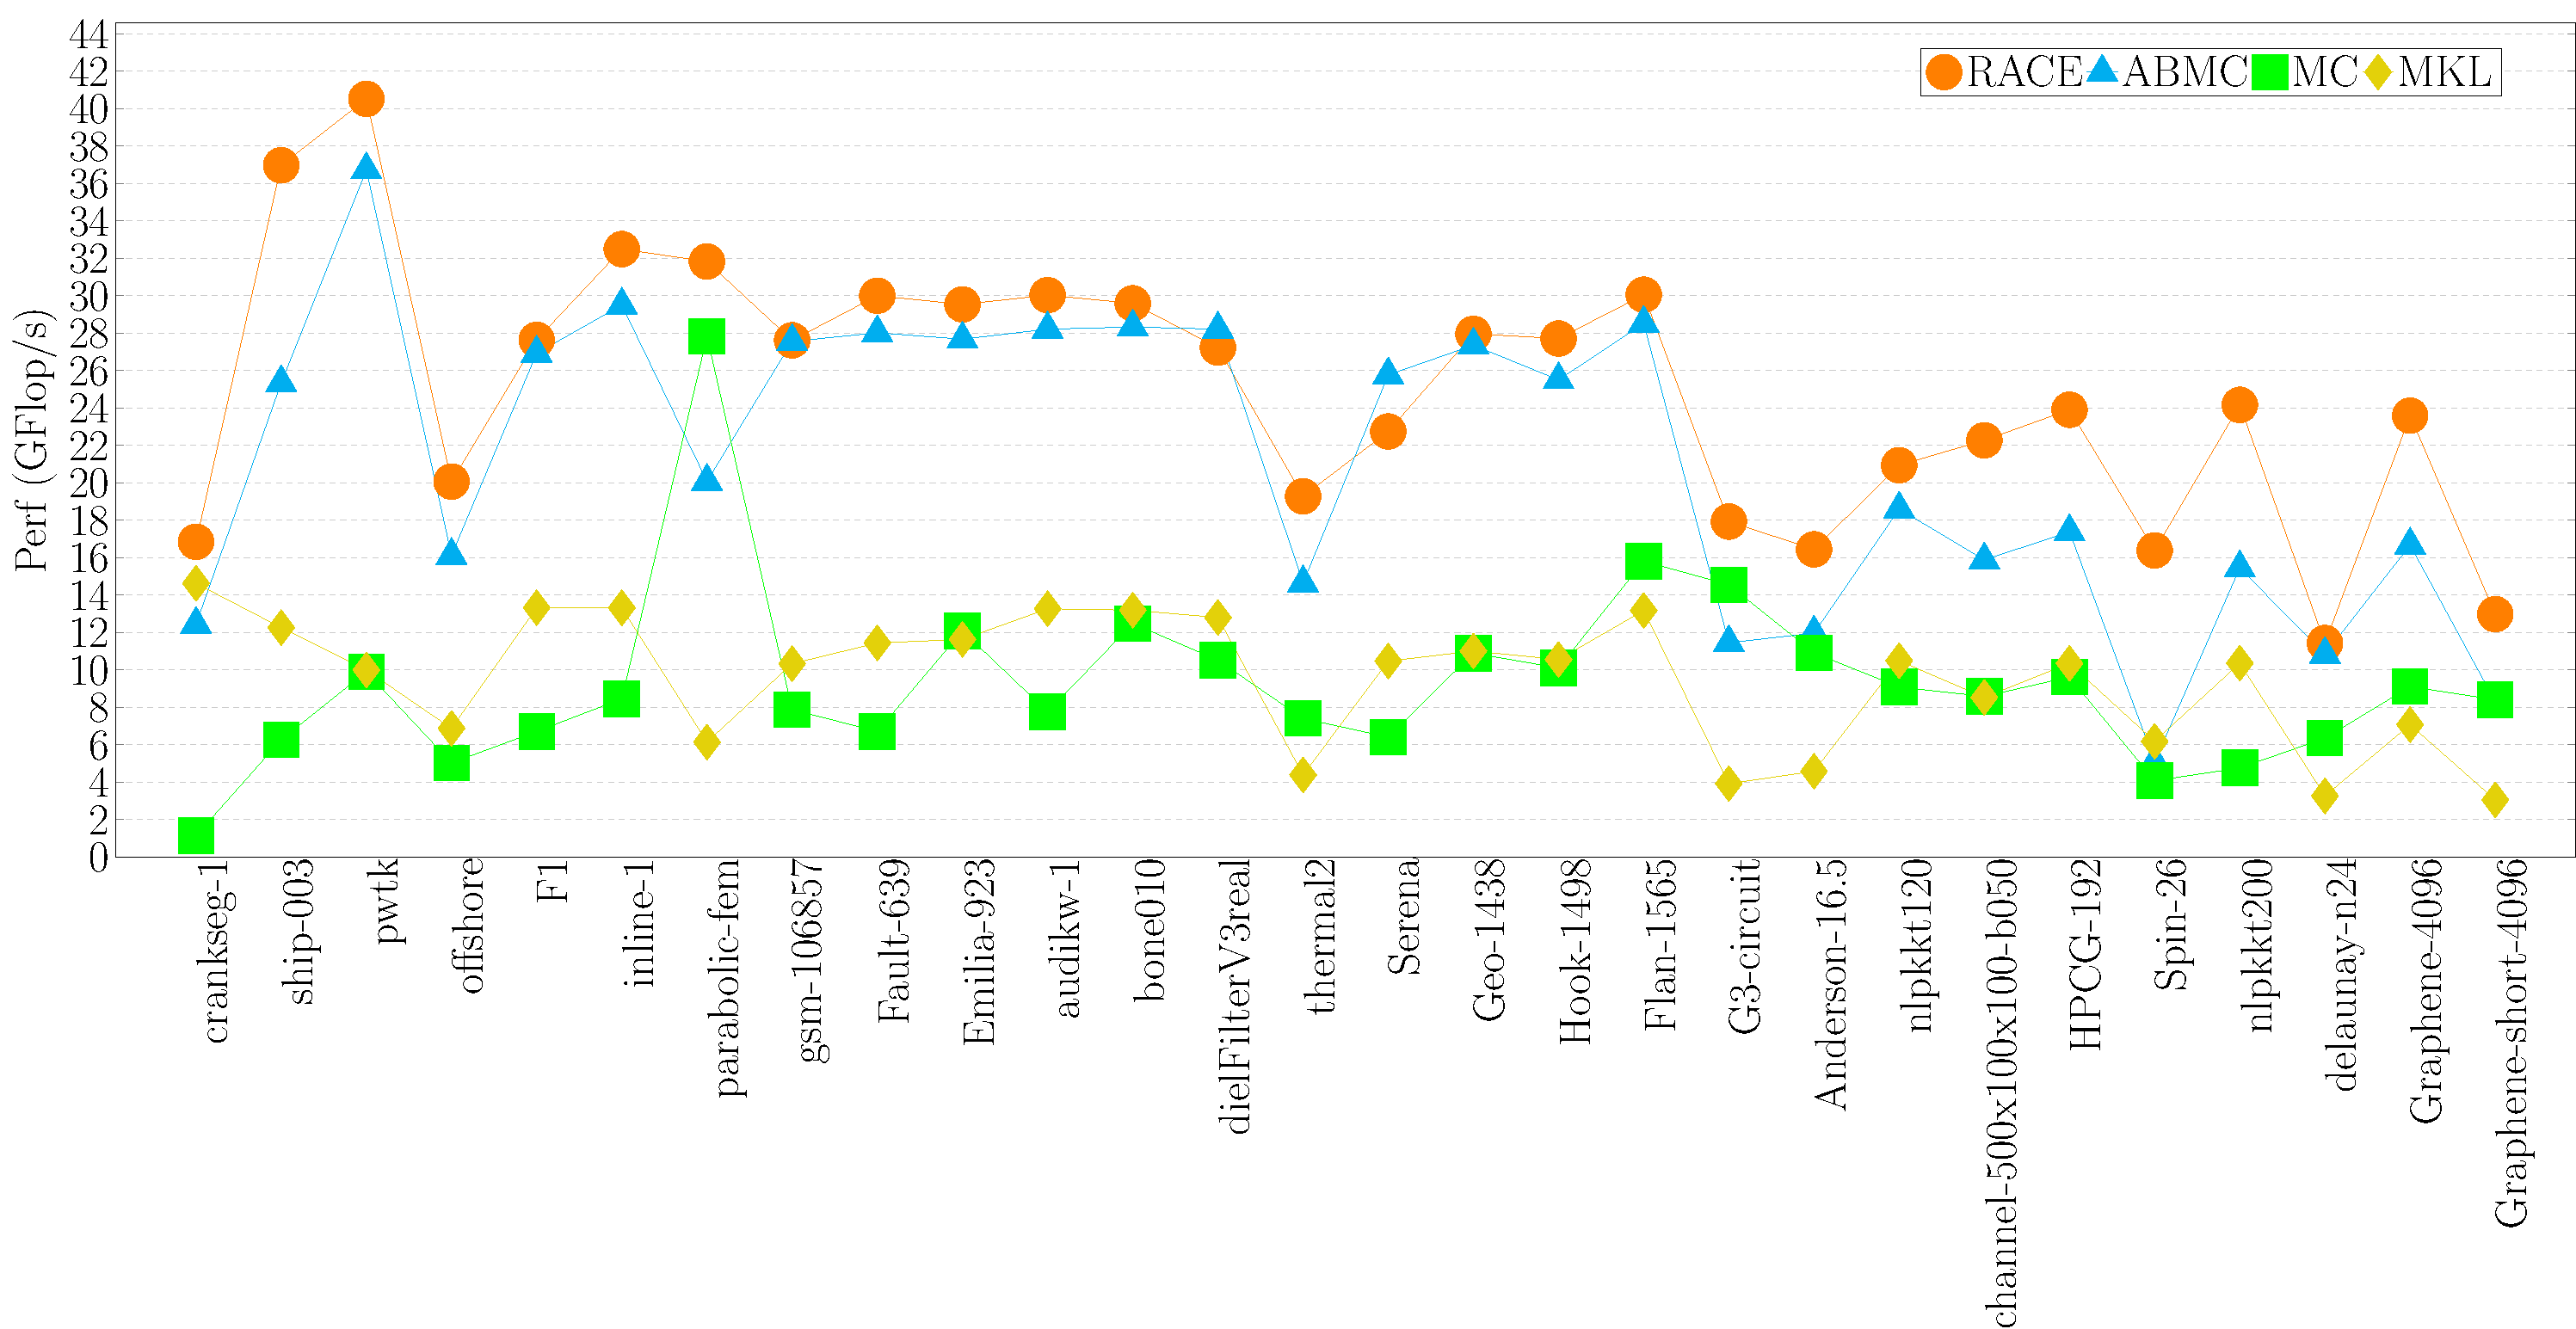
\includegraphics[width=0.85\textwidth, height=0.27\textheight]{pics/results/skx/data_symm_spmv/plot_generator/perf_vs_mtx/perf}}
	\caption{\SymmSpmv performance}
	\label{fig:symm_spmv}
\end{figure}

\begin{comment}

\begin{figure}[thbp]
	\centering
	\subfloat[\SymmSpmv on 1 socket of \IVB]{\label{fig:symm_spmv_ivy_nlpkkt}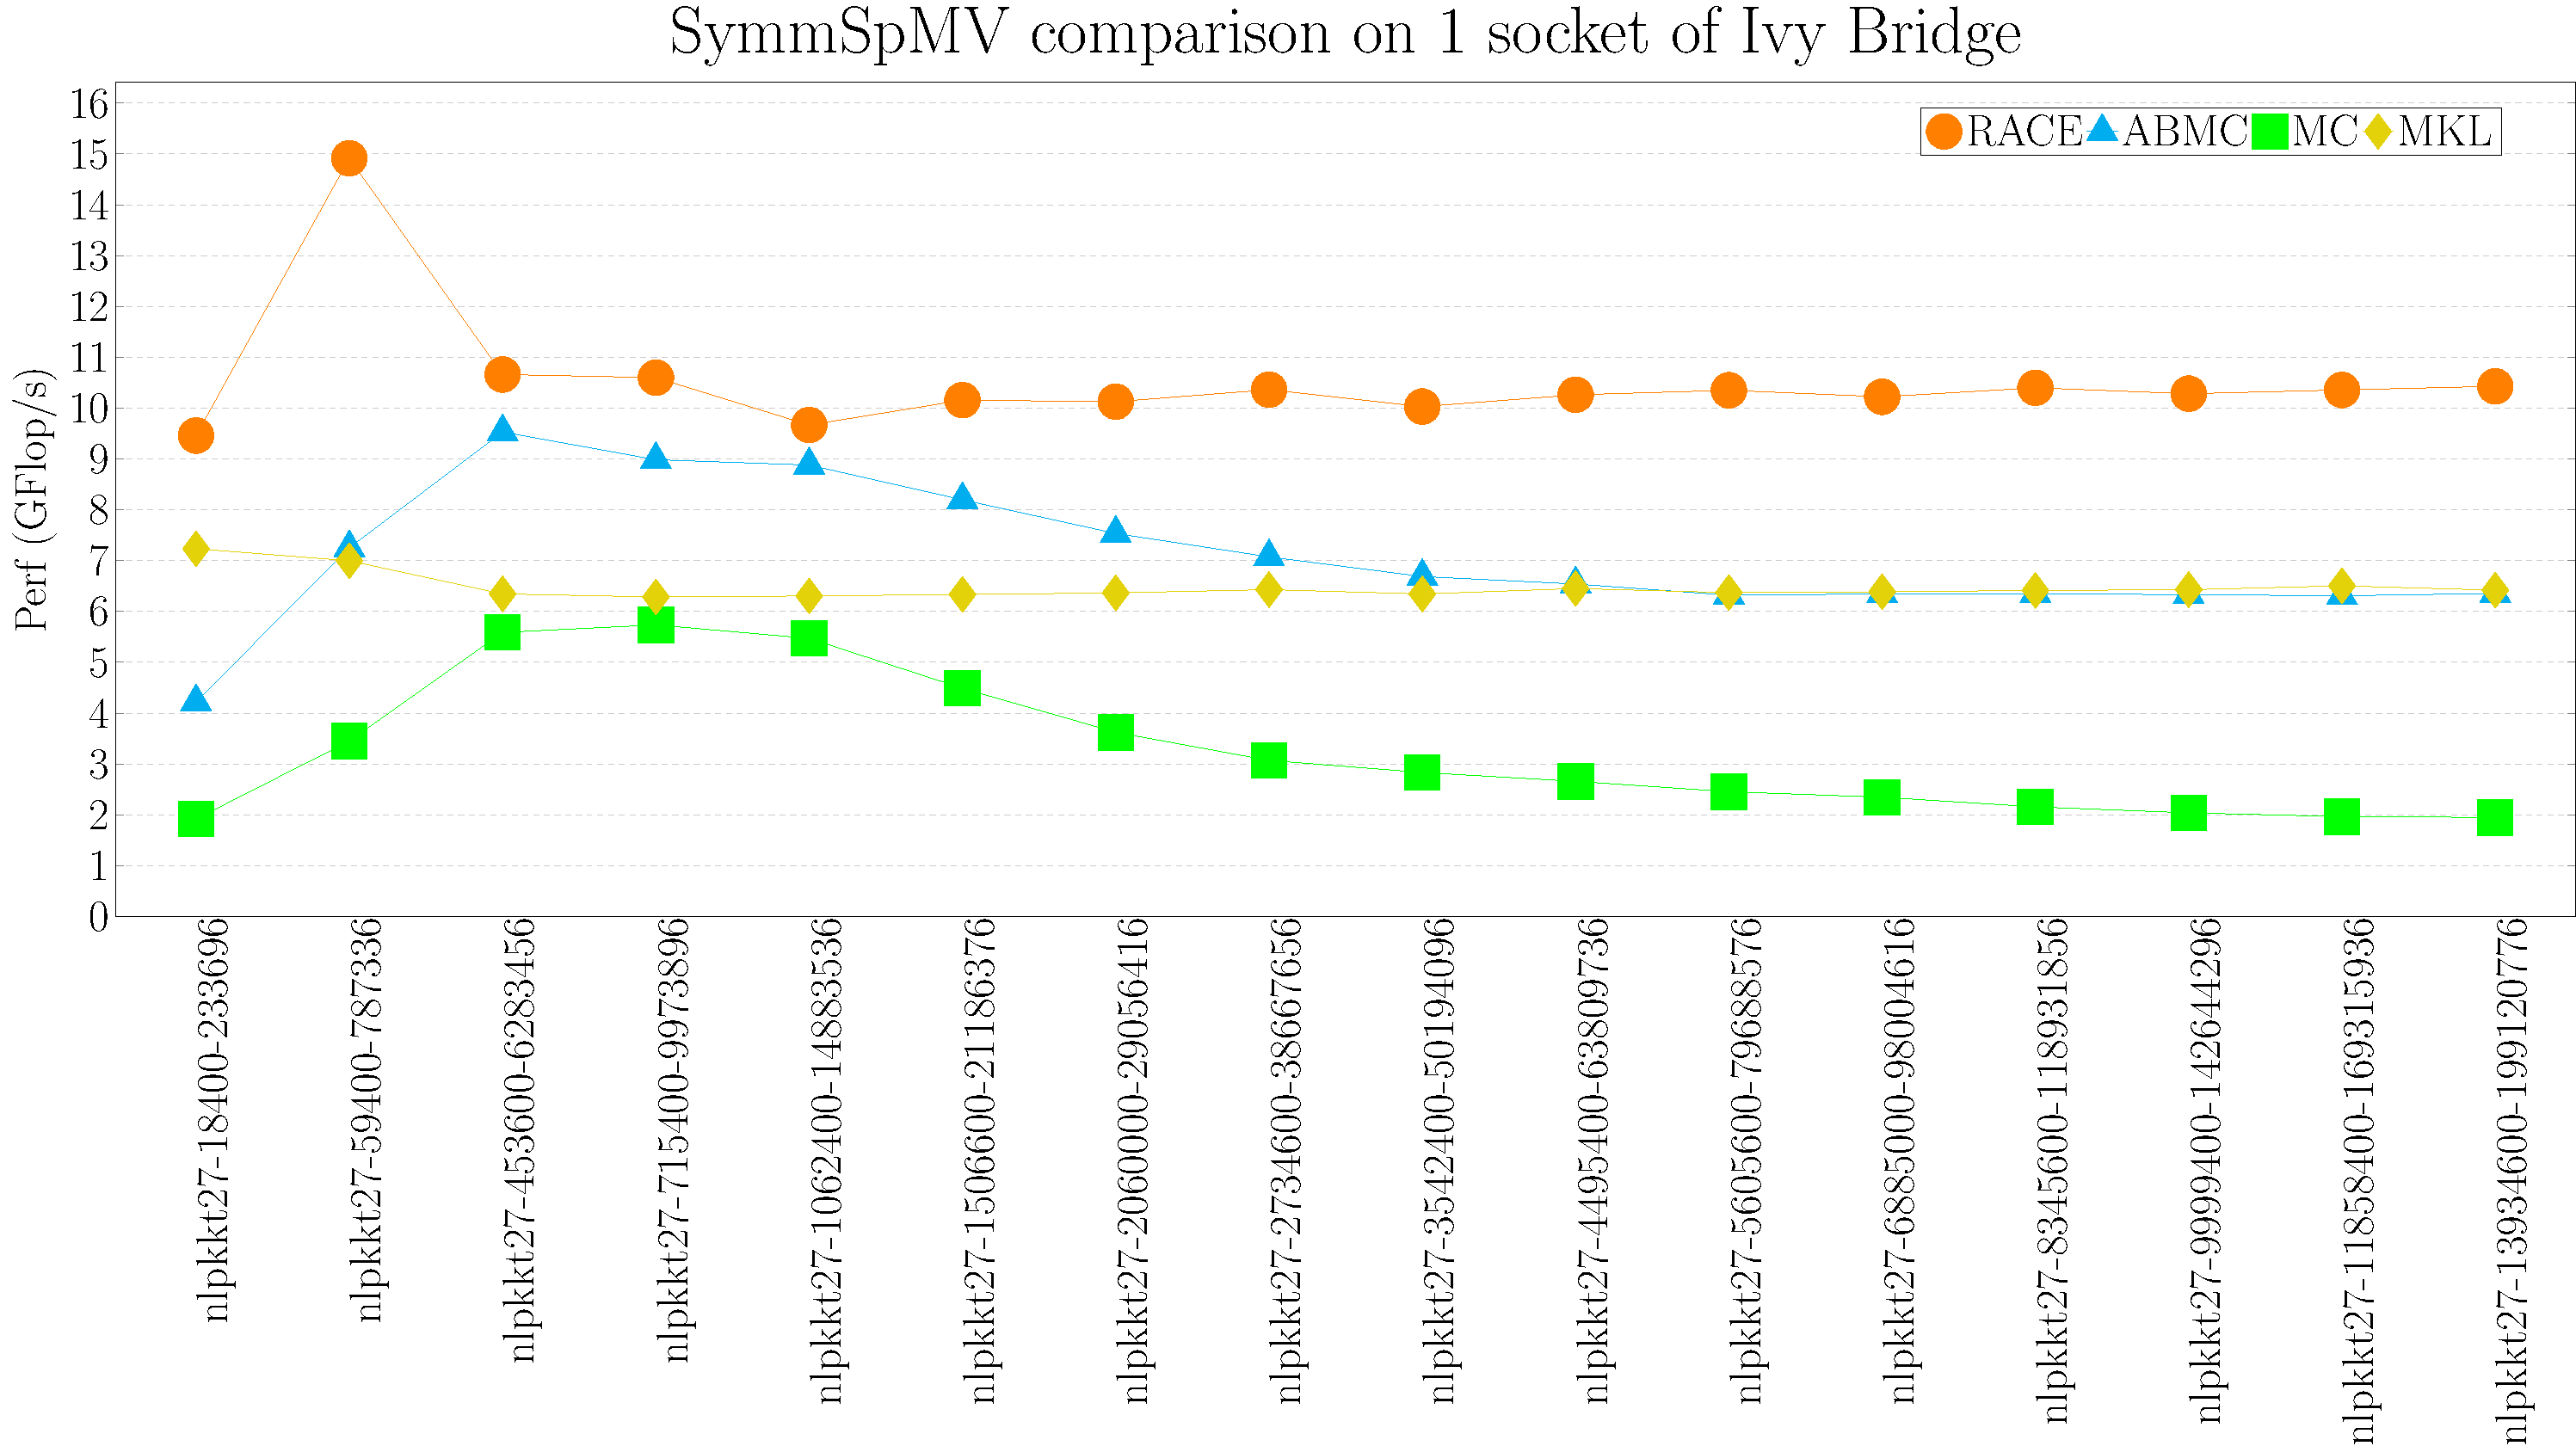
\includegraphics[width=0.48\textwidth, height=0.15\textheight]{pics/results/ivy/data_symm_spmv/plot_generator/perf_vs_mtx/ivy_nlpkkt}}
	\hspace{1em}
	\subfloat[\SymmSpmv on 1 socket of \SKX]{\label{fig:symm_spmv_skx_nlpkkt}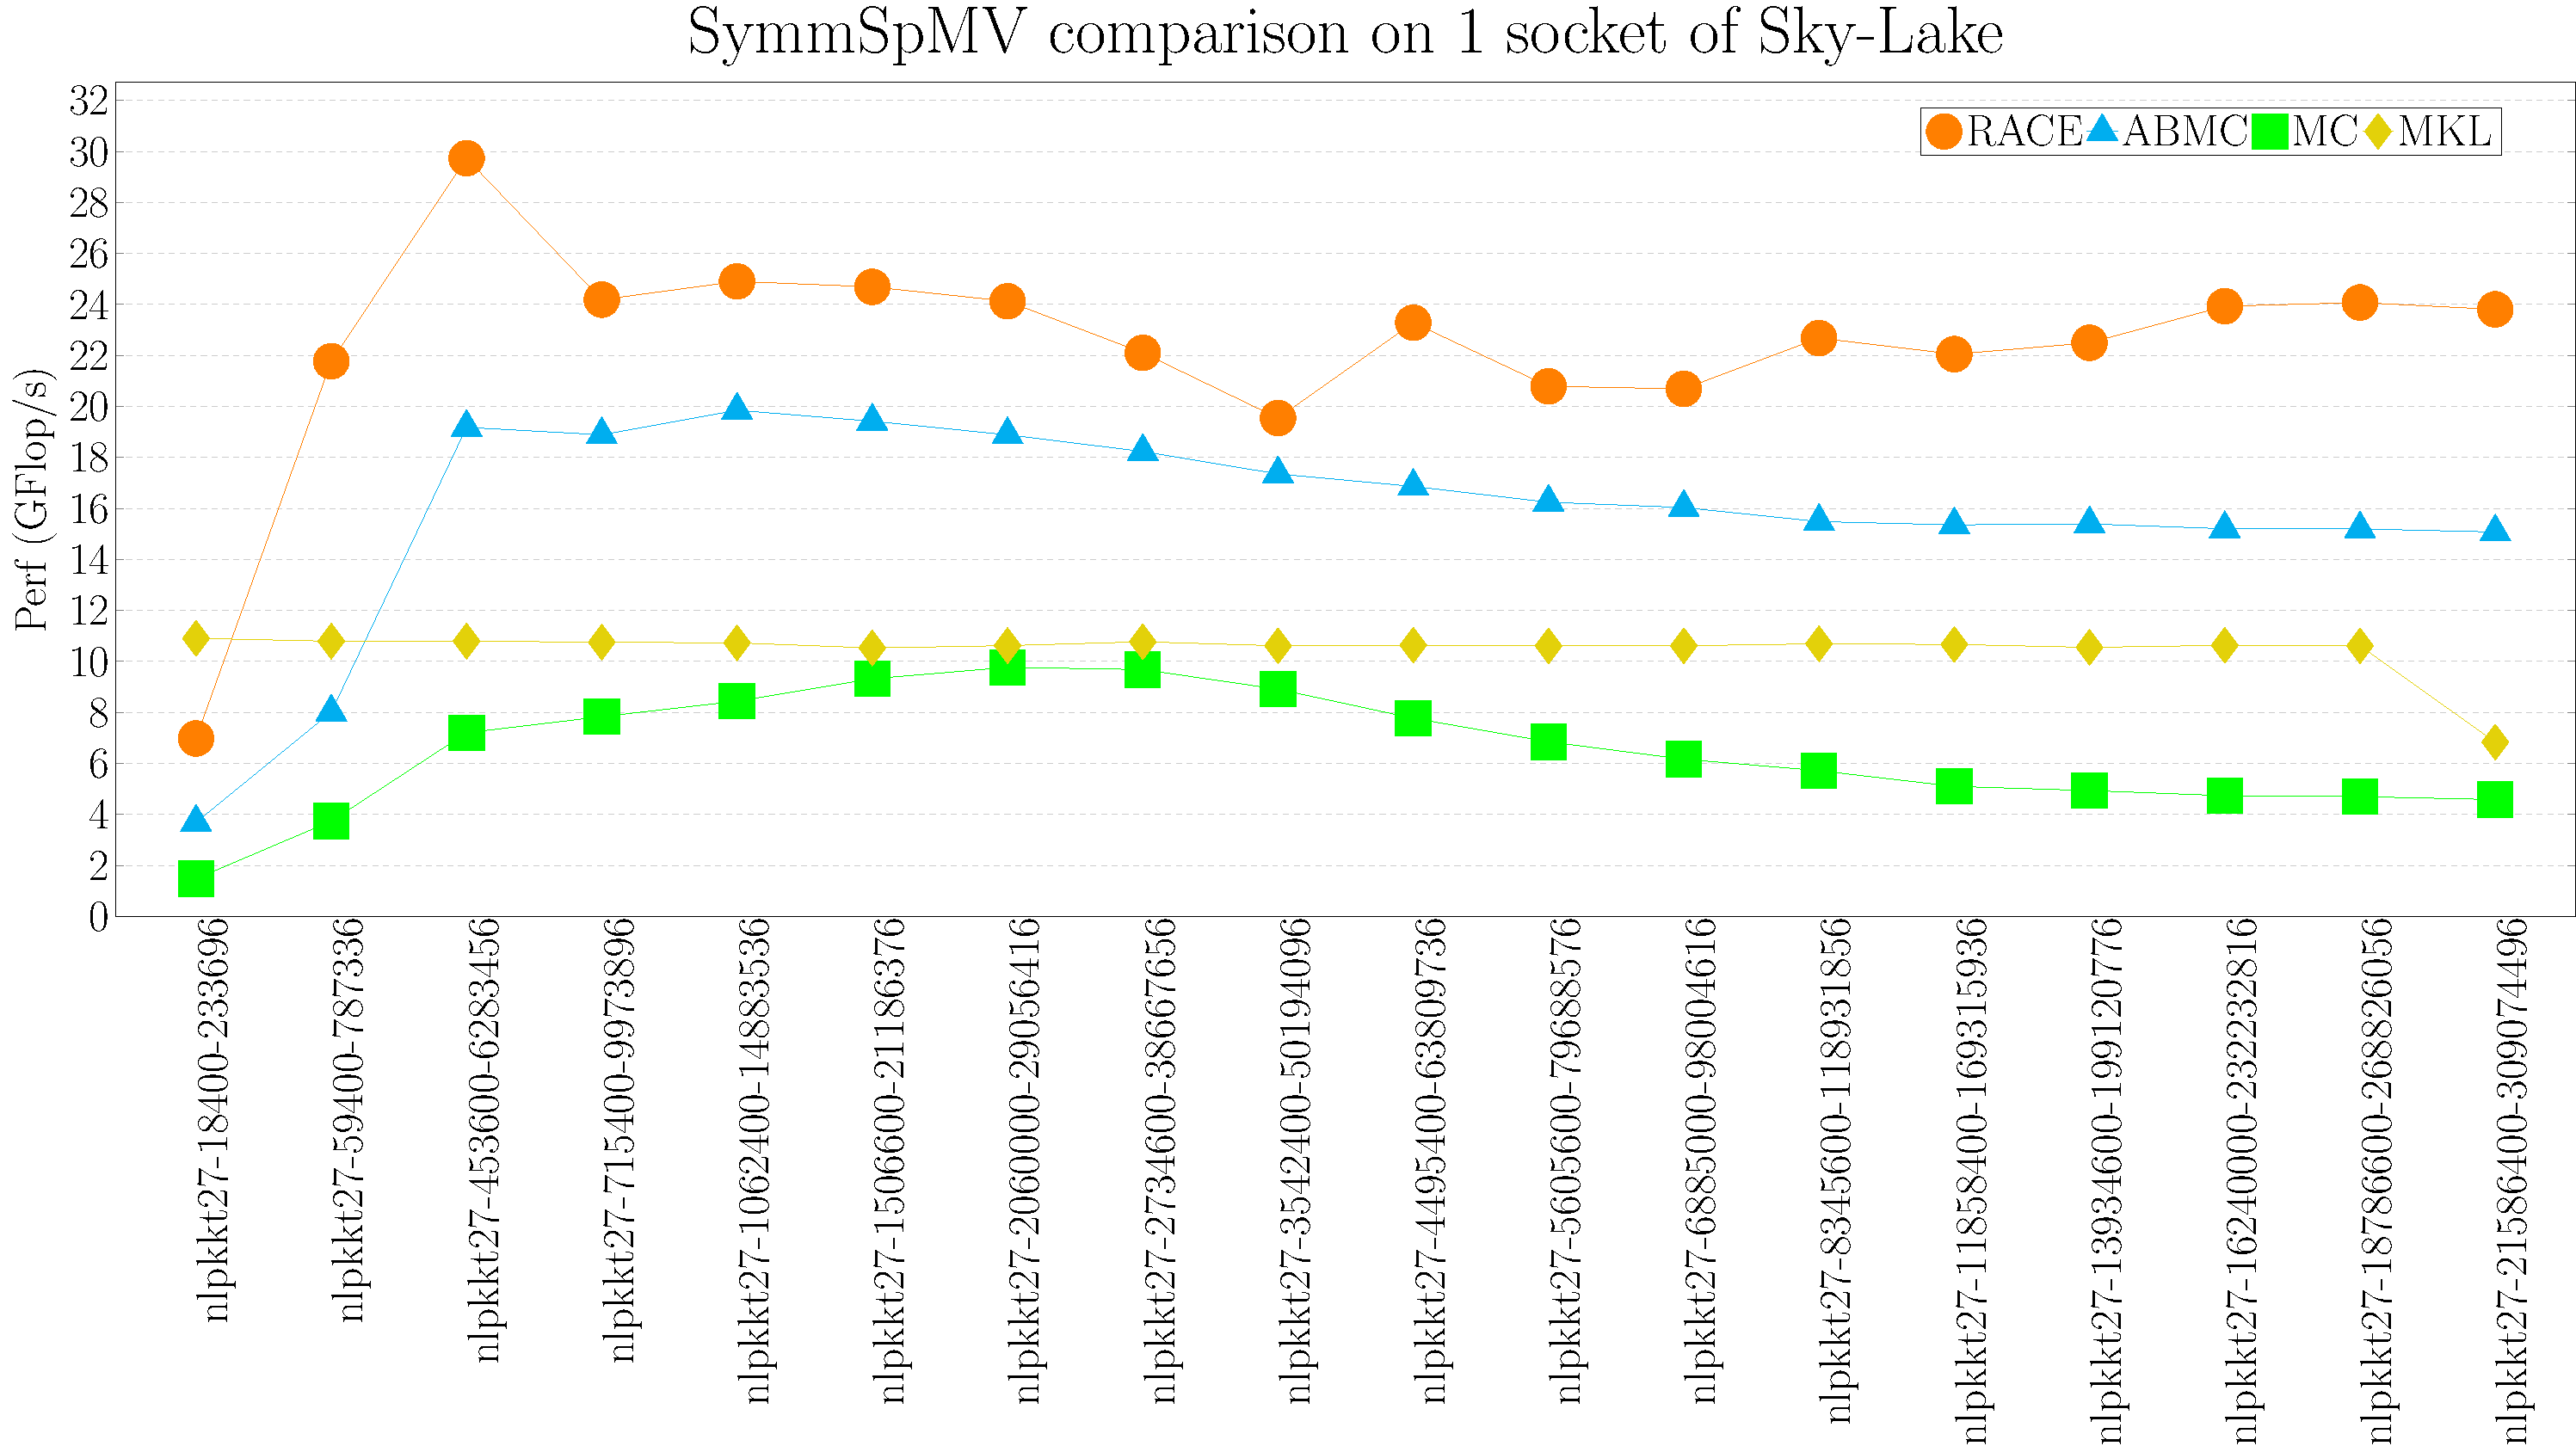
\includegraphics[width=0.48\textwidth, height=0.15\textheight]{pics/results/skx/data_symm_spmv/plot_generator/perf_vs_mtx/skx_nlpkkt}}
	\caption{\SymmSpmv performance for nlpkkt matrices}
	\label{fig:symm_spmv_nlpkkt}
\end{figure}

\begin{figure}[thbp]
	\centering
	\subfloat[\SymmSpmv on 1 socket of \IVB]{\label{fig:symm_spmv_ivy_scamac}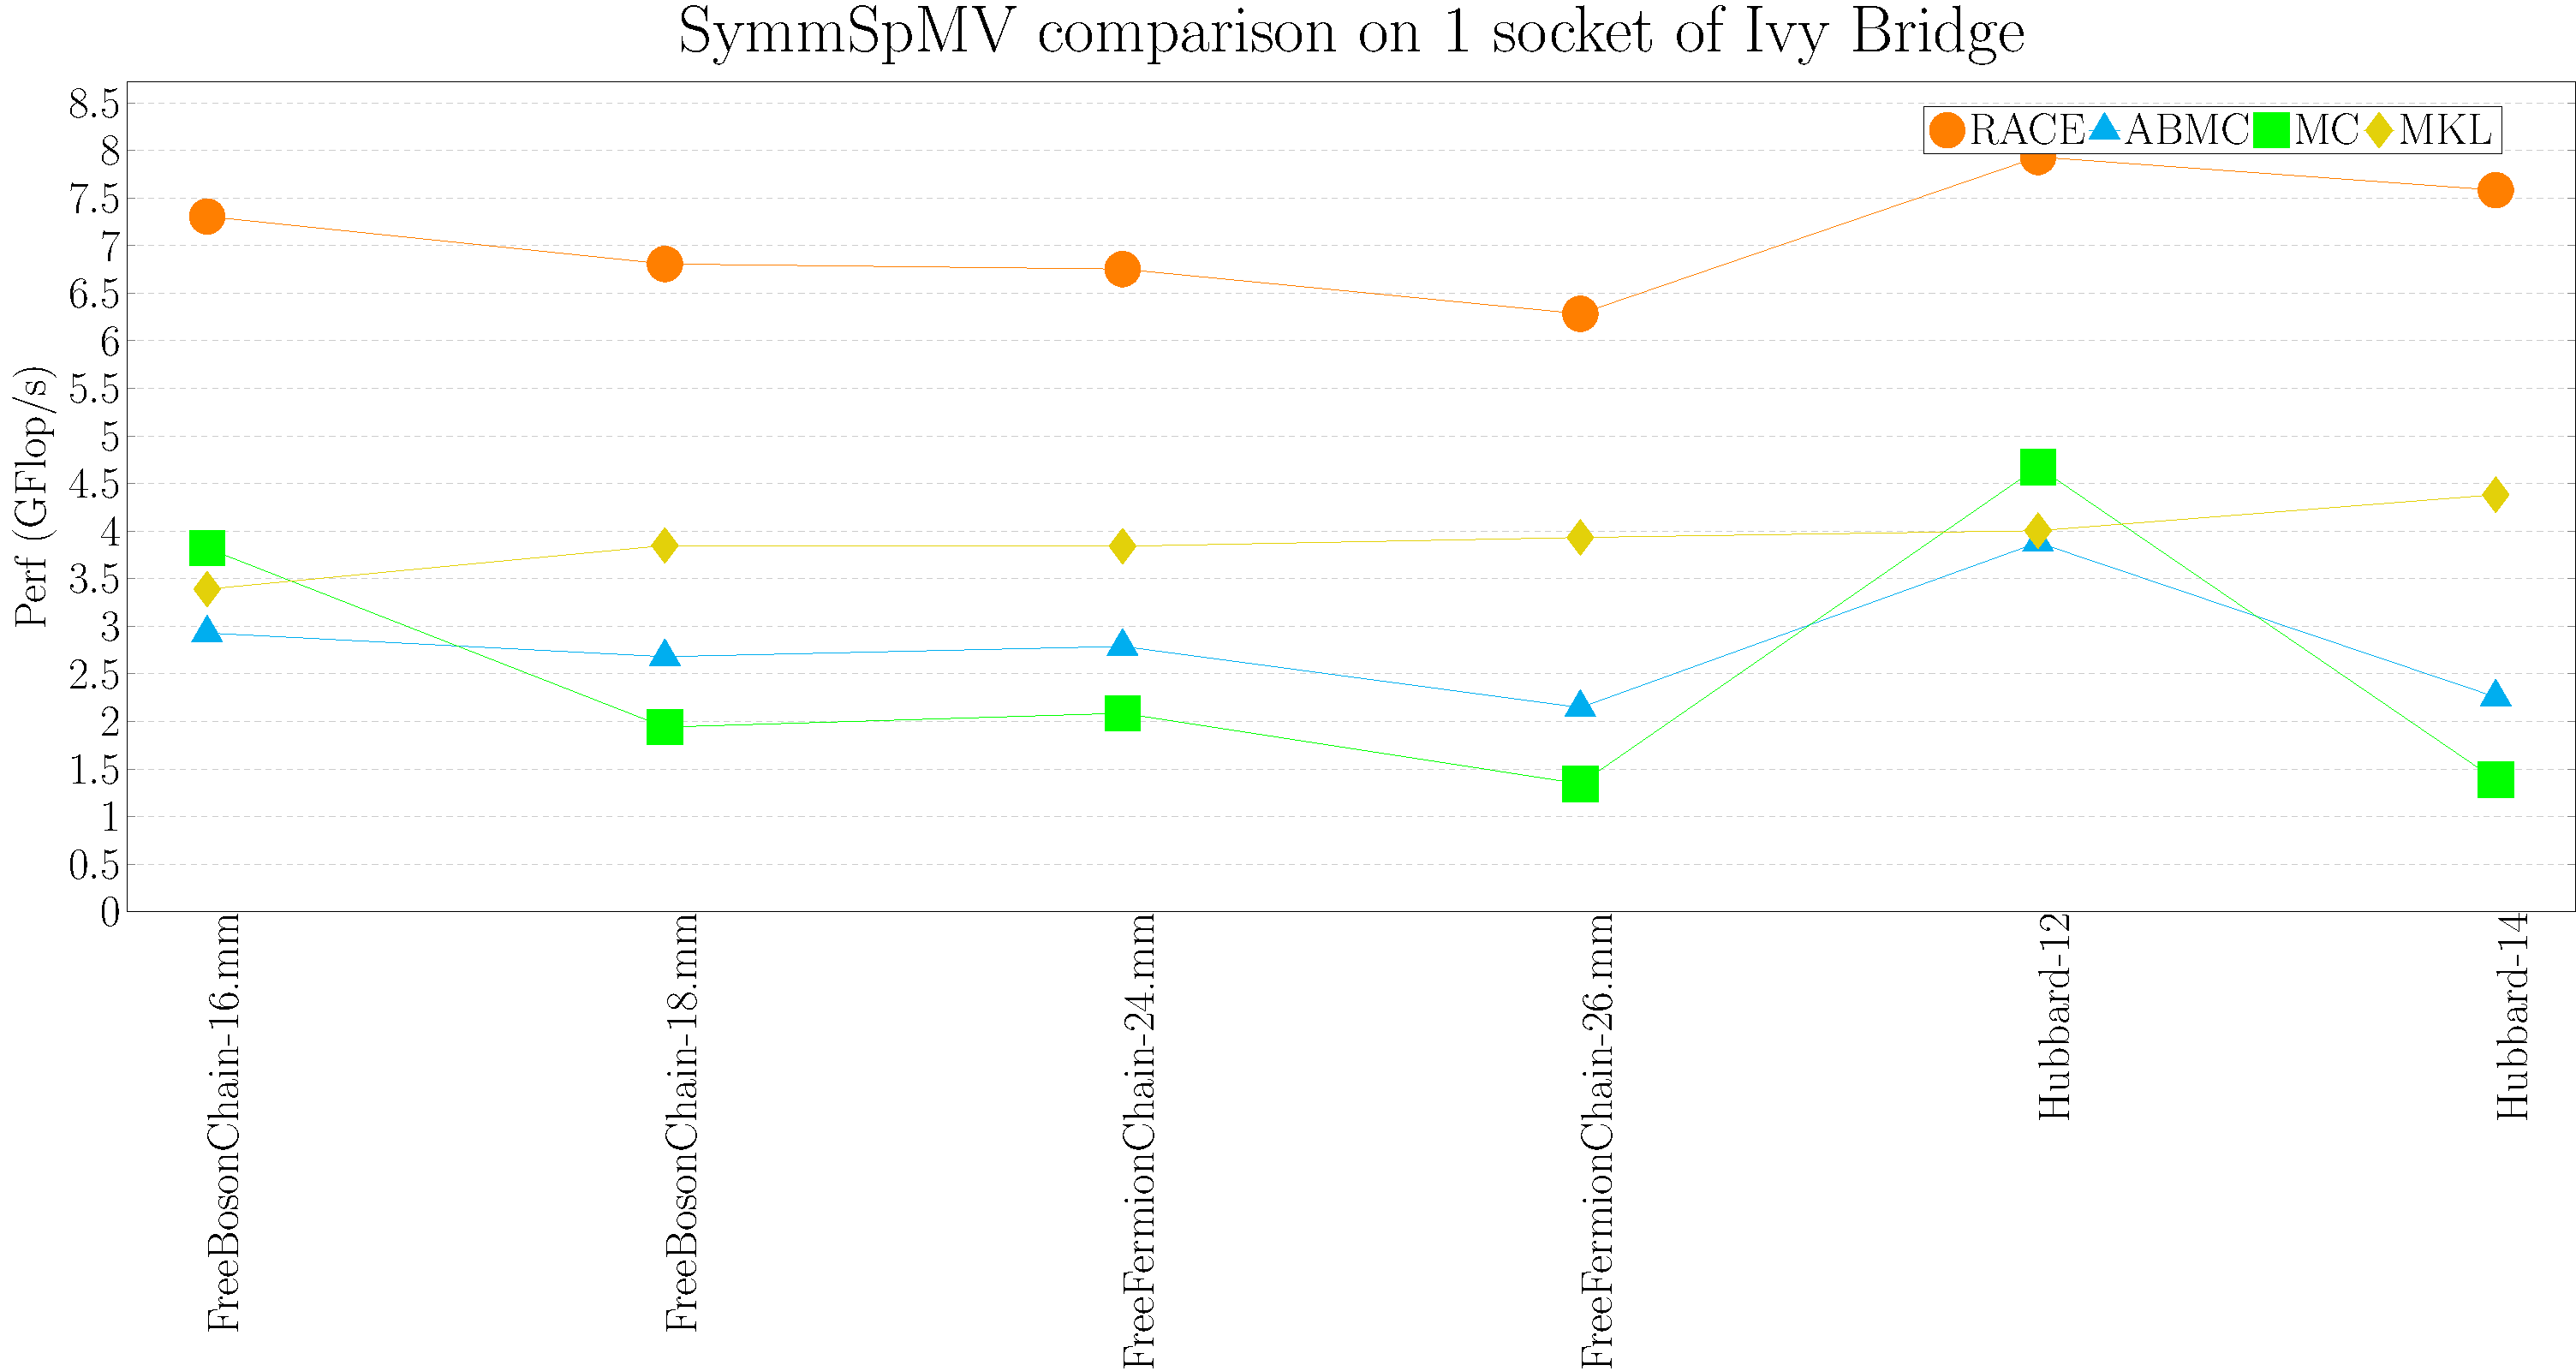
\includegraphics[width=0.48\textwidth, height=0.15\textheight]{pics/results/ivy/data_symm_spmv/plot_generator/perf_vs_mtx/ivy_scamac}}
	\hspace{1em}
	\subfloat[\SymmSpmv on 1 socket of \SKX]{\label{fig:symm_spmv_skx_scamac}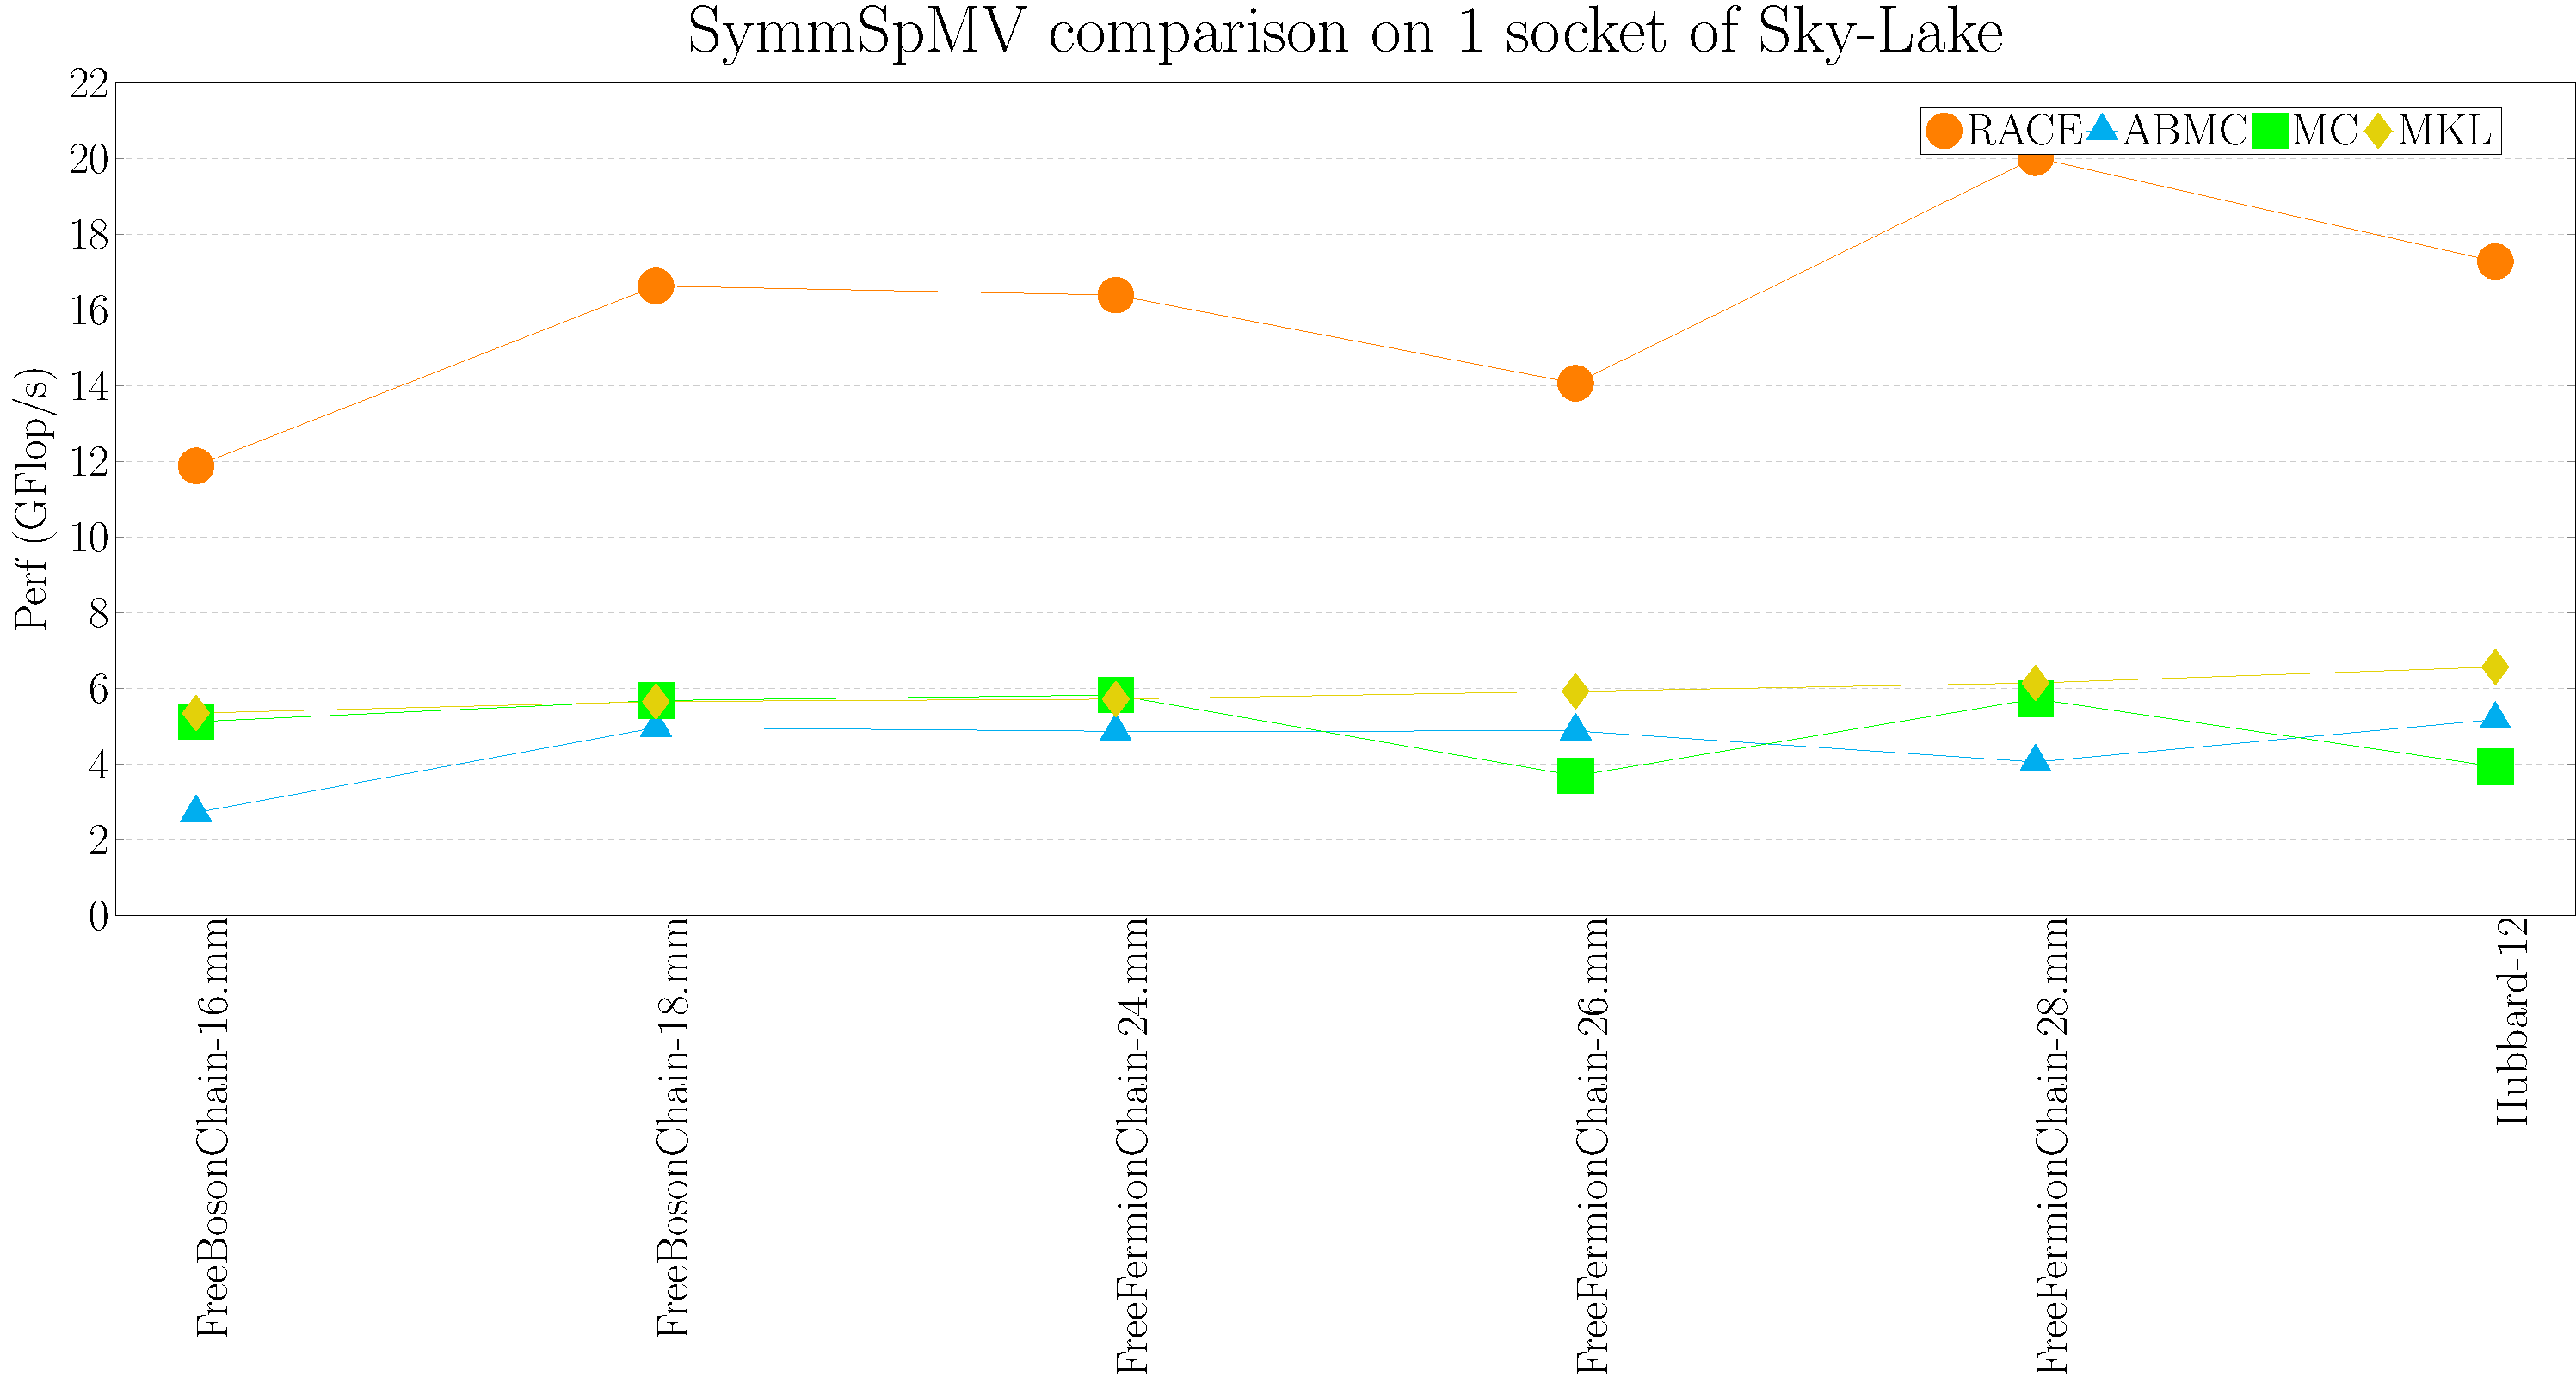
\includegraphics[width=0.48\textwidth, height=0.15\textheight]{pics/results/skx/data_symm_spmv/plot_generator/perf_vs_mtx/skx_scamac}}
	\caption{\SymmSpmv performance for SCAMAC matrices}
	\label{fig:symm_spmv_scamac}
\end{figure}

\end{comment}

%\begin{figure}[thbp]
%	\centering
	%\subfloat[RACE performance compared to SpMV]{\label{fig:race_skx}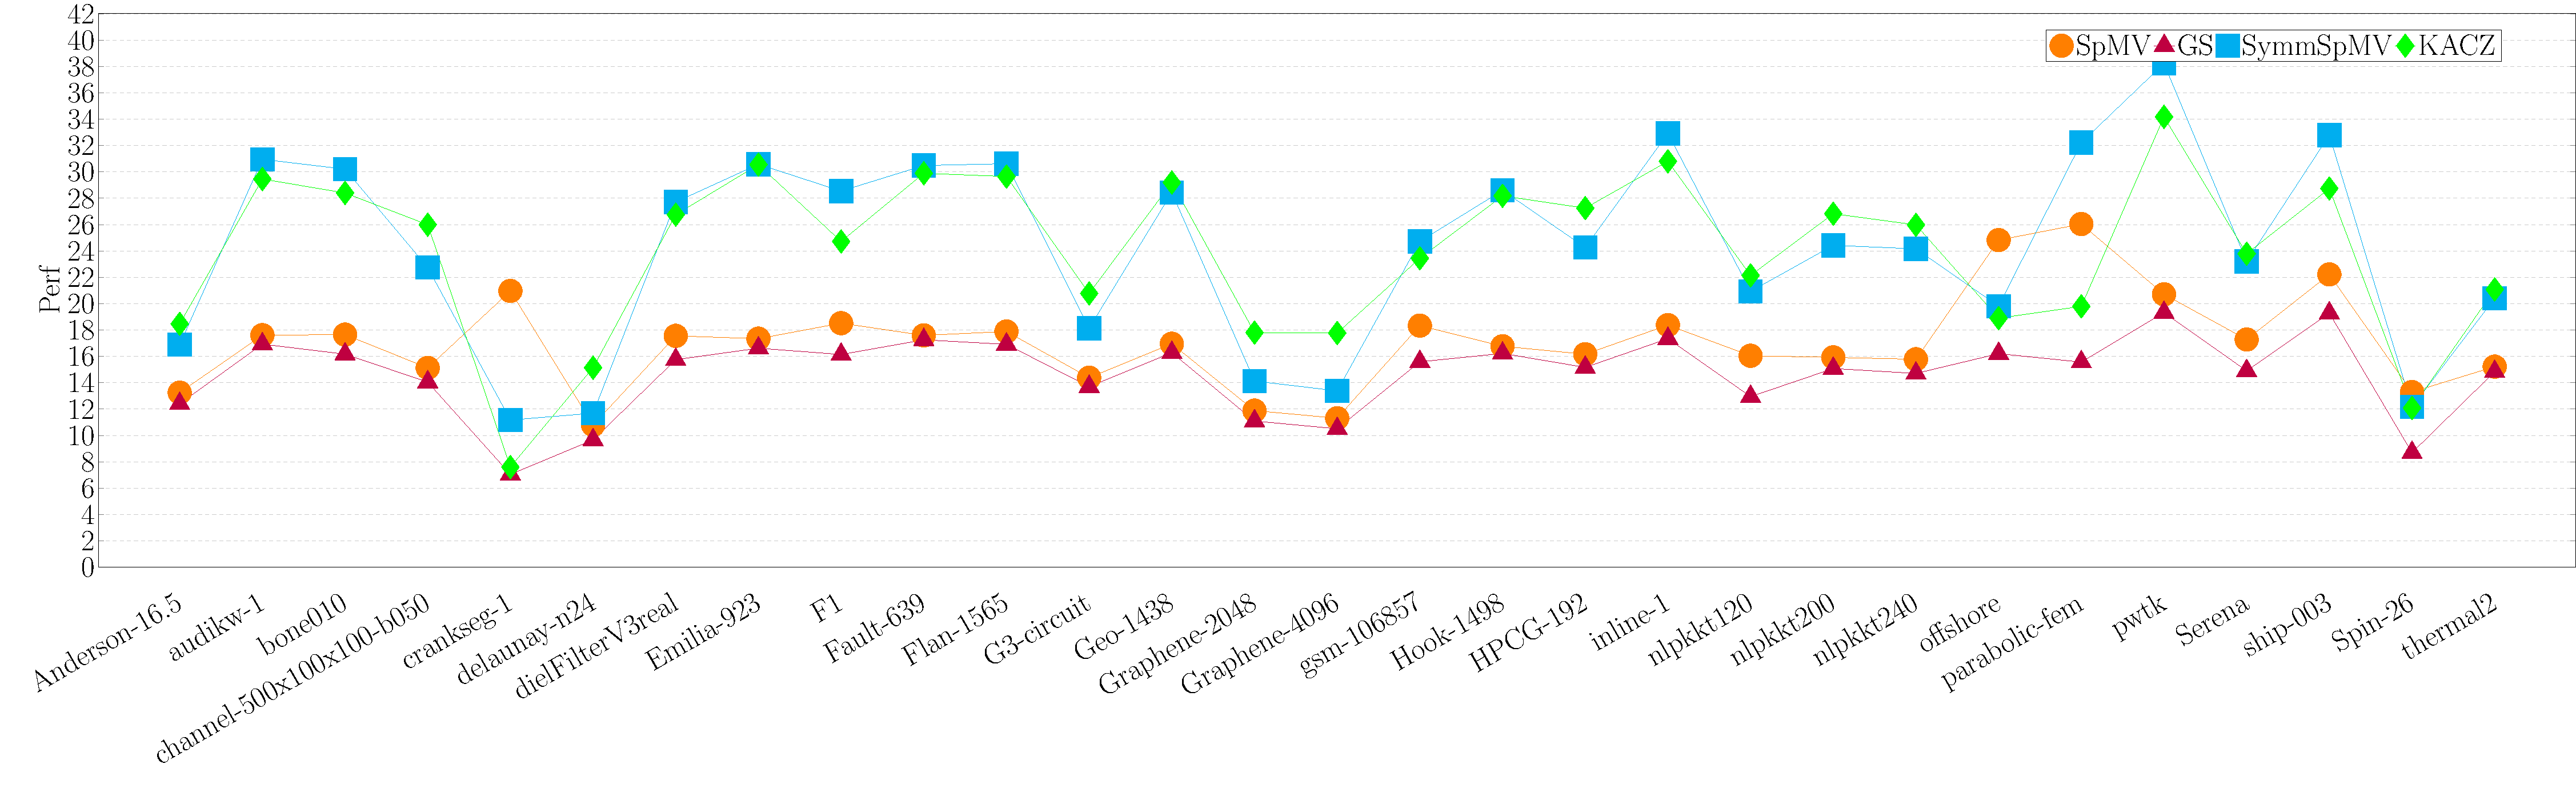
\includegraphics[width=0.45\textwidth, height=0.15\textheight]{pics/results/skx/race}}
	%\hspace{1.2em}
%	\subfloat[SymmSpMV Comparison]{\label{fig:symm_spmv_skx}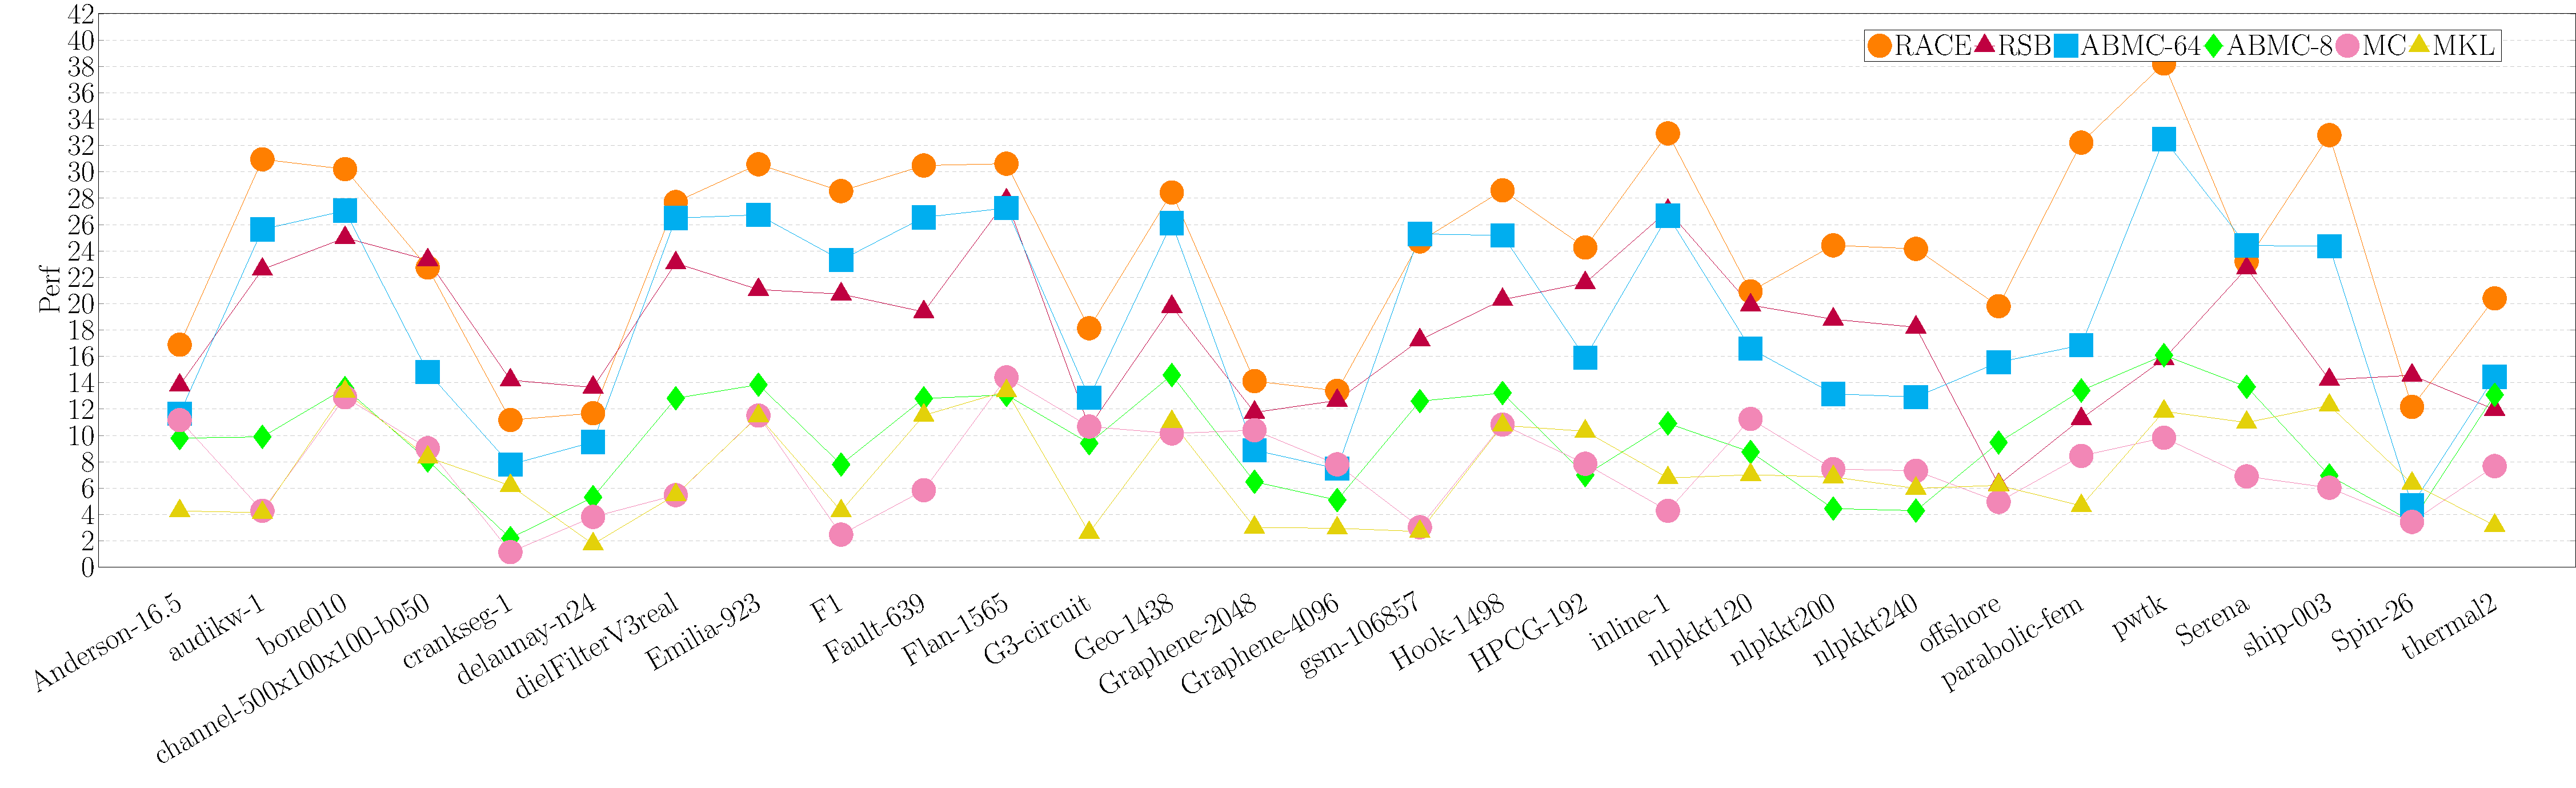
\includegraphics[width=0.45\textwidth, height=0.15\textheight]{pics/results/skx/symm_spmv}}
%	\hspace{1.2em}
	%\subfloat[GS Comparison]{\label{fig:gs_skx}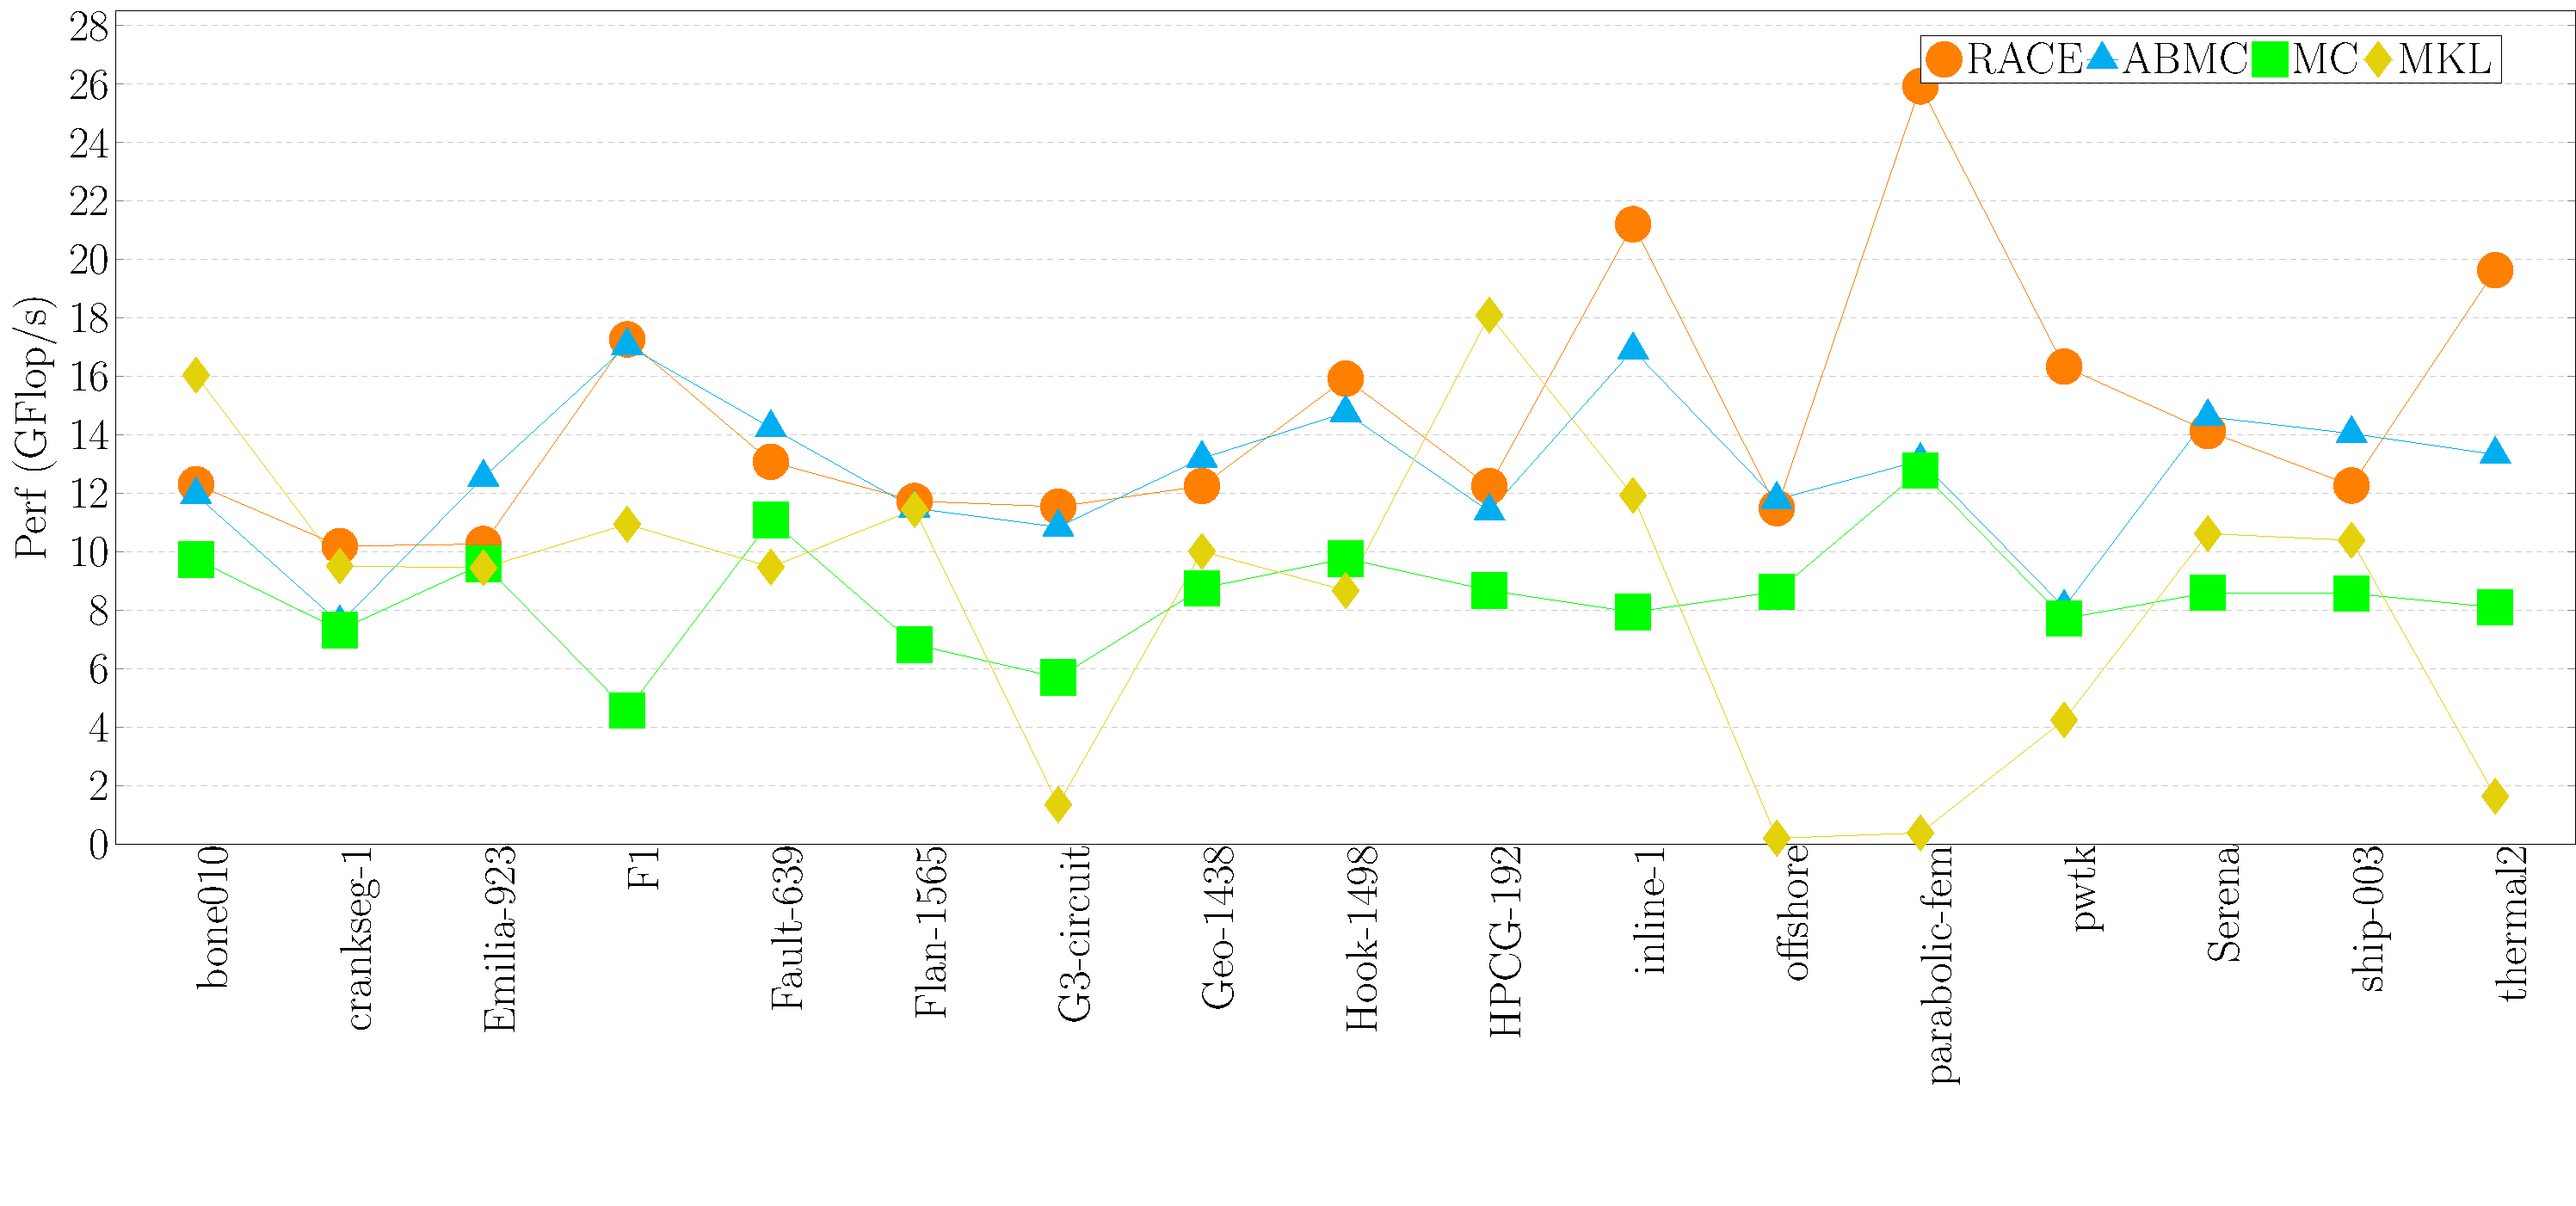
\includegraphics[width=0.45\textwidth, height=0.15\textheight]{pics/results/skx/gs}}
	%\hspace{1.2em}
%	\subfloat[KACZ Comparison]{\label{fig:kacz_skx}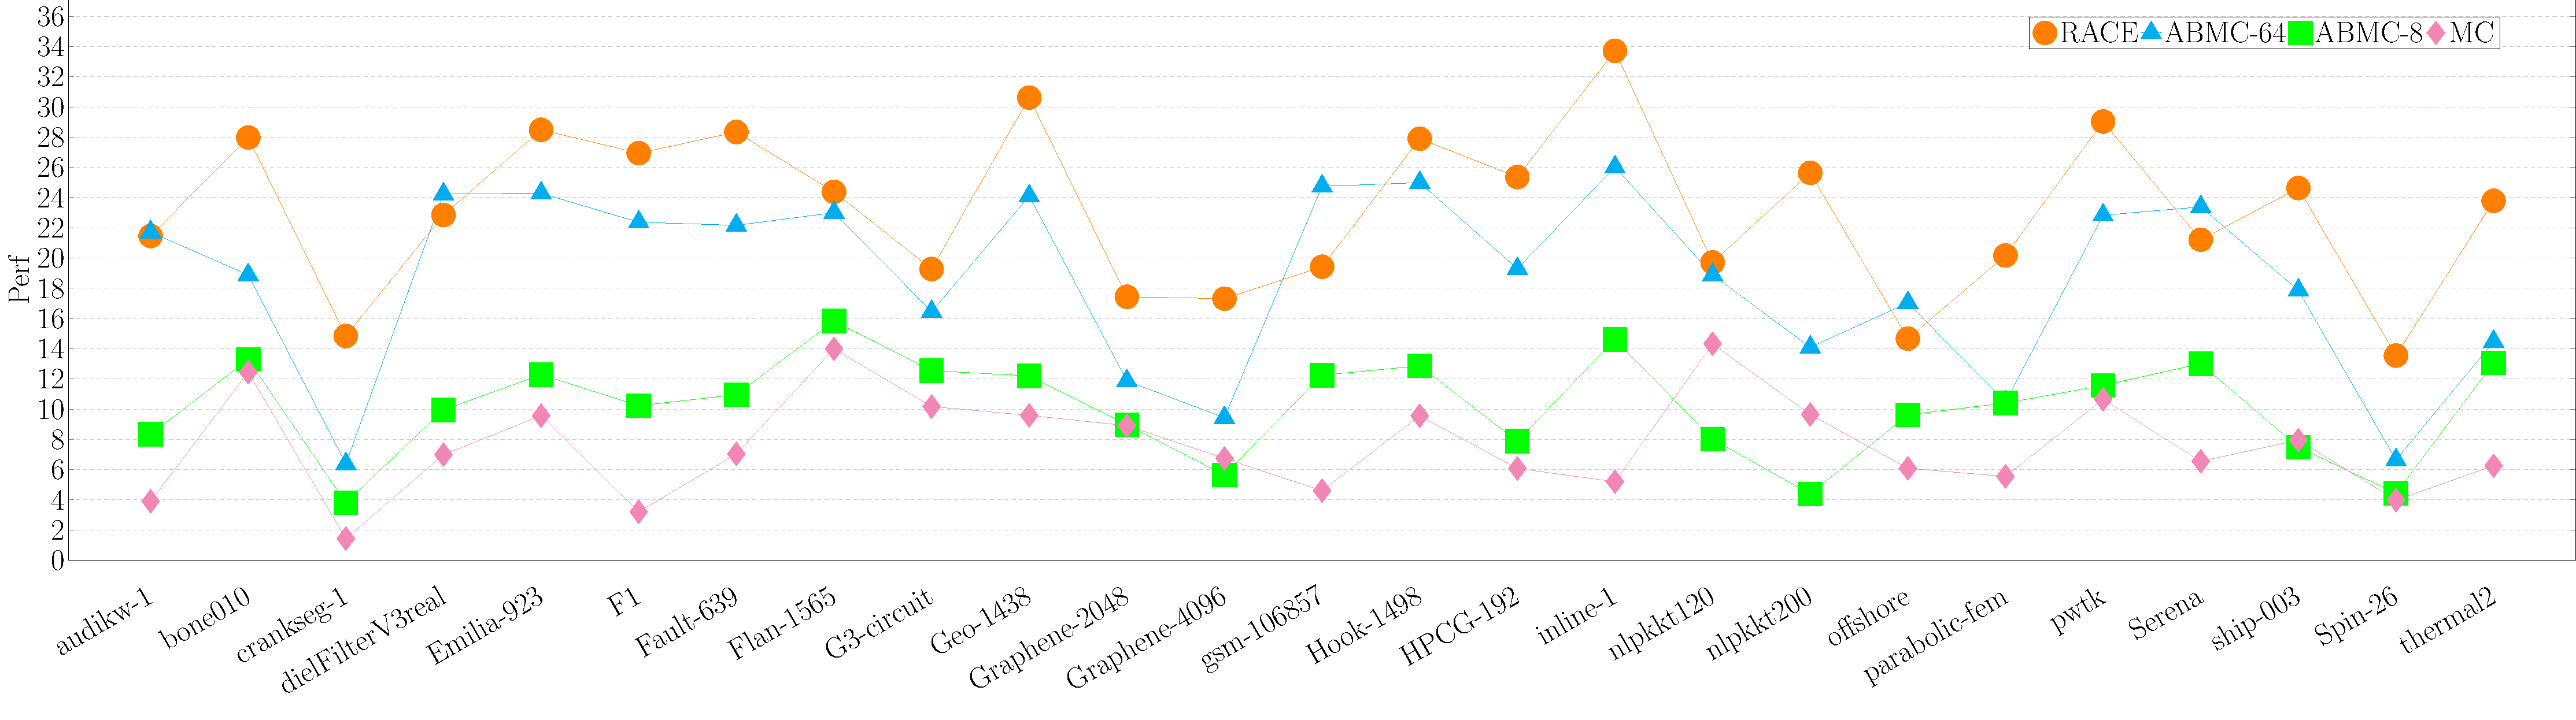
\includegraphics[width=0.45\textwidth, height=0.15\textheight]{pics/results/skx/kacz}}
%	\caption{Performance results on \SKX}
%	\label{fig:skx}
%\end{figure}

%\subsubsection{RACE performance}
%Here we plot the performance of \SymmSpmv, \GS and \KACZ with \RACE compared to \SpMV. \Cref{fig:race_ivy,fig:race_skx} will be used here. This is done for entire test matrices and all the hardwares. 

\subsubsection{Exact kernel}
Here we compare  \RACE with \ABMC, \MC and \MKL for \SymmSpmv. \Cref{fig:symm_spmv_ivy,fig:symm_spmv_skx} will be used. \COLPACK \cite{COLPACK} %TOD cite
was used for multicoloring (\MC). \METIS \cite{METIS}  was used for graph partitioning for \ABMC, and \COLPACK was used for coloring the hyper graph. The blocksize for \ABMC is chosen by doing parameter scan over 4 to 128 as shown by Iwashita \etal in \cite{ABMC}, and choosing the optimal one. Note that the time for this parameter search is not included in the performance results shown. 


\begin{figure}[thbp]
	\centering
	\subfloat[1 socket \IVB] {\label{fig:derived_perf_kacz_ivb}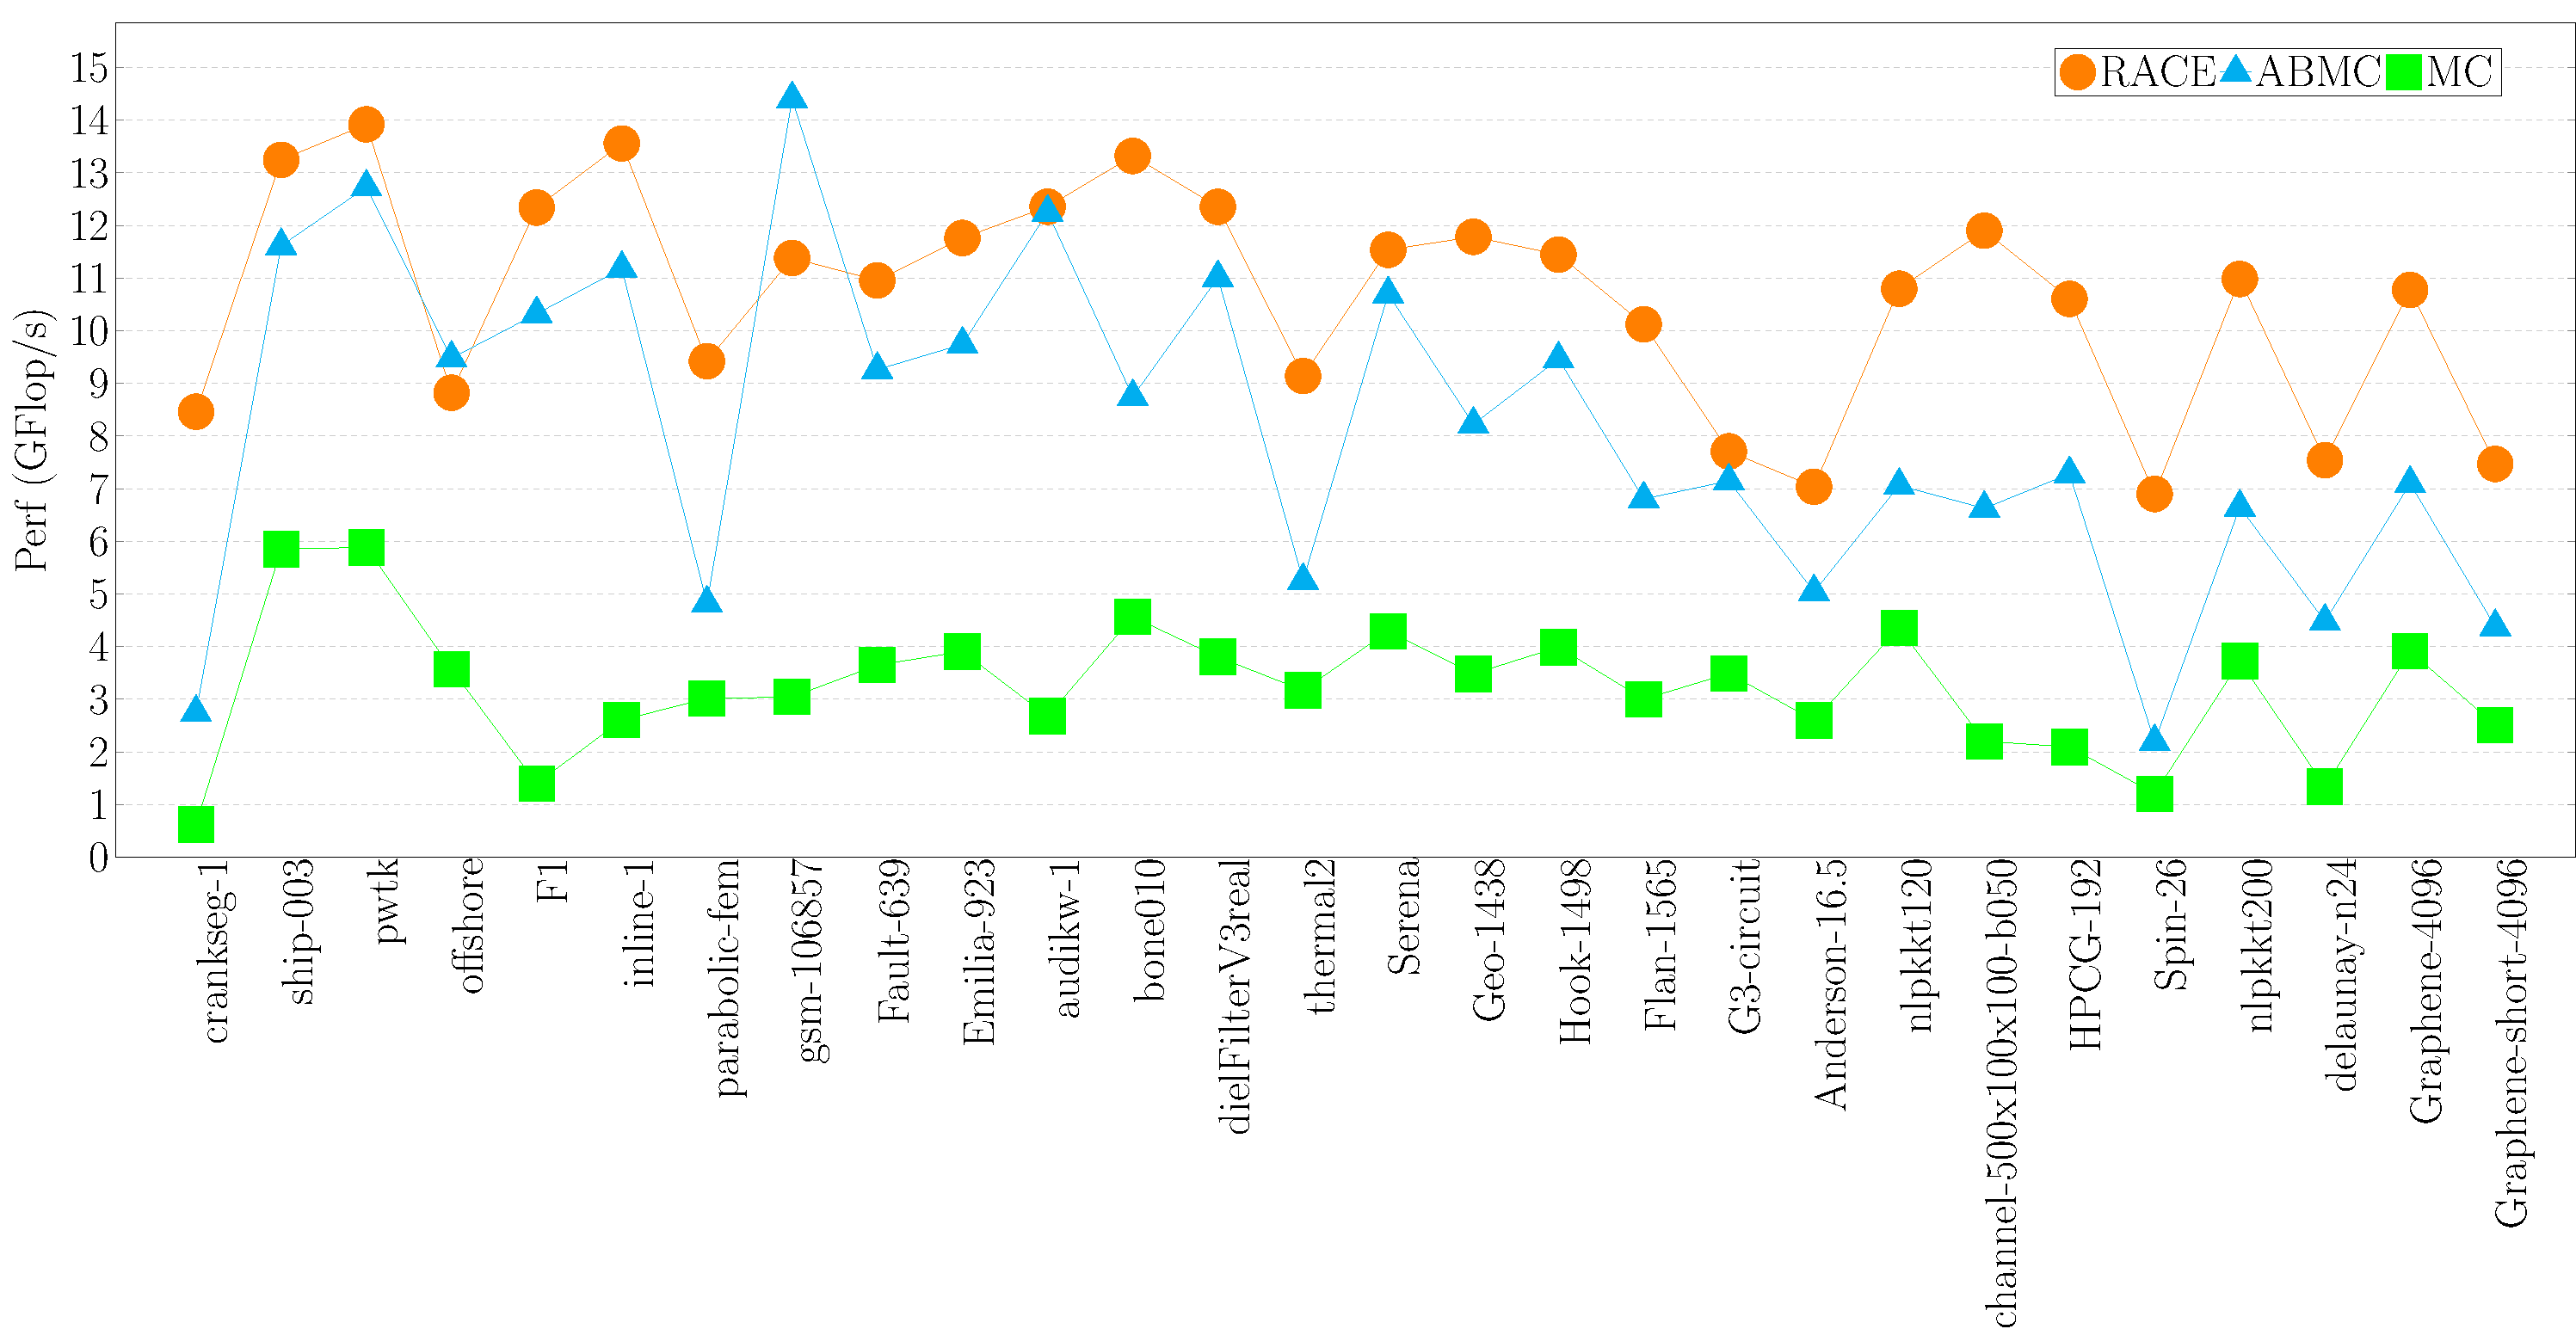
\includegraphics[width=0.85\textwidth, height=0.27\textheight]{pics/results/ivy/data_symm_kacz/plot_generator/derived_perf_vs_mtx/derived_perf}}
	\hspace{1em}
	\subfloat[1 socket \SKX] {\label{fig:derived_perf_kacz_skx}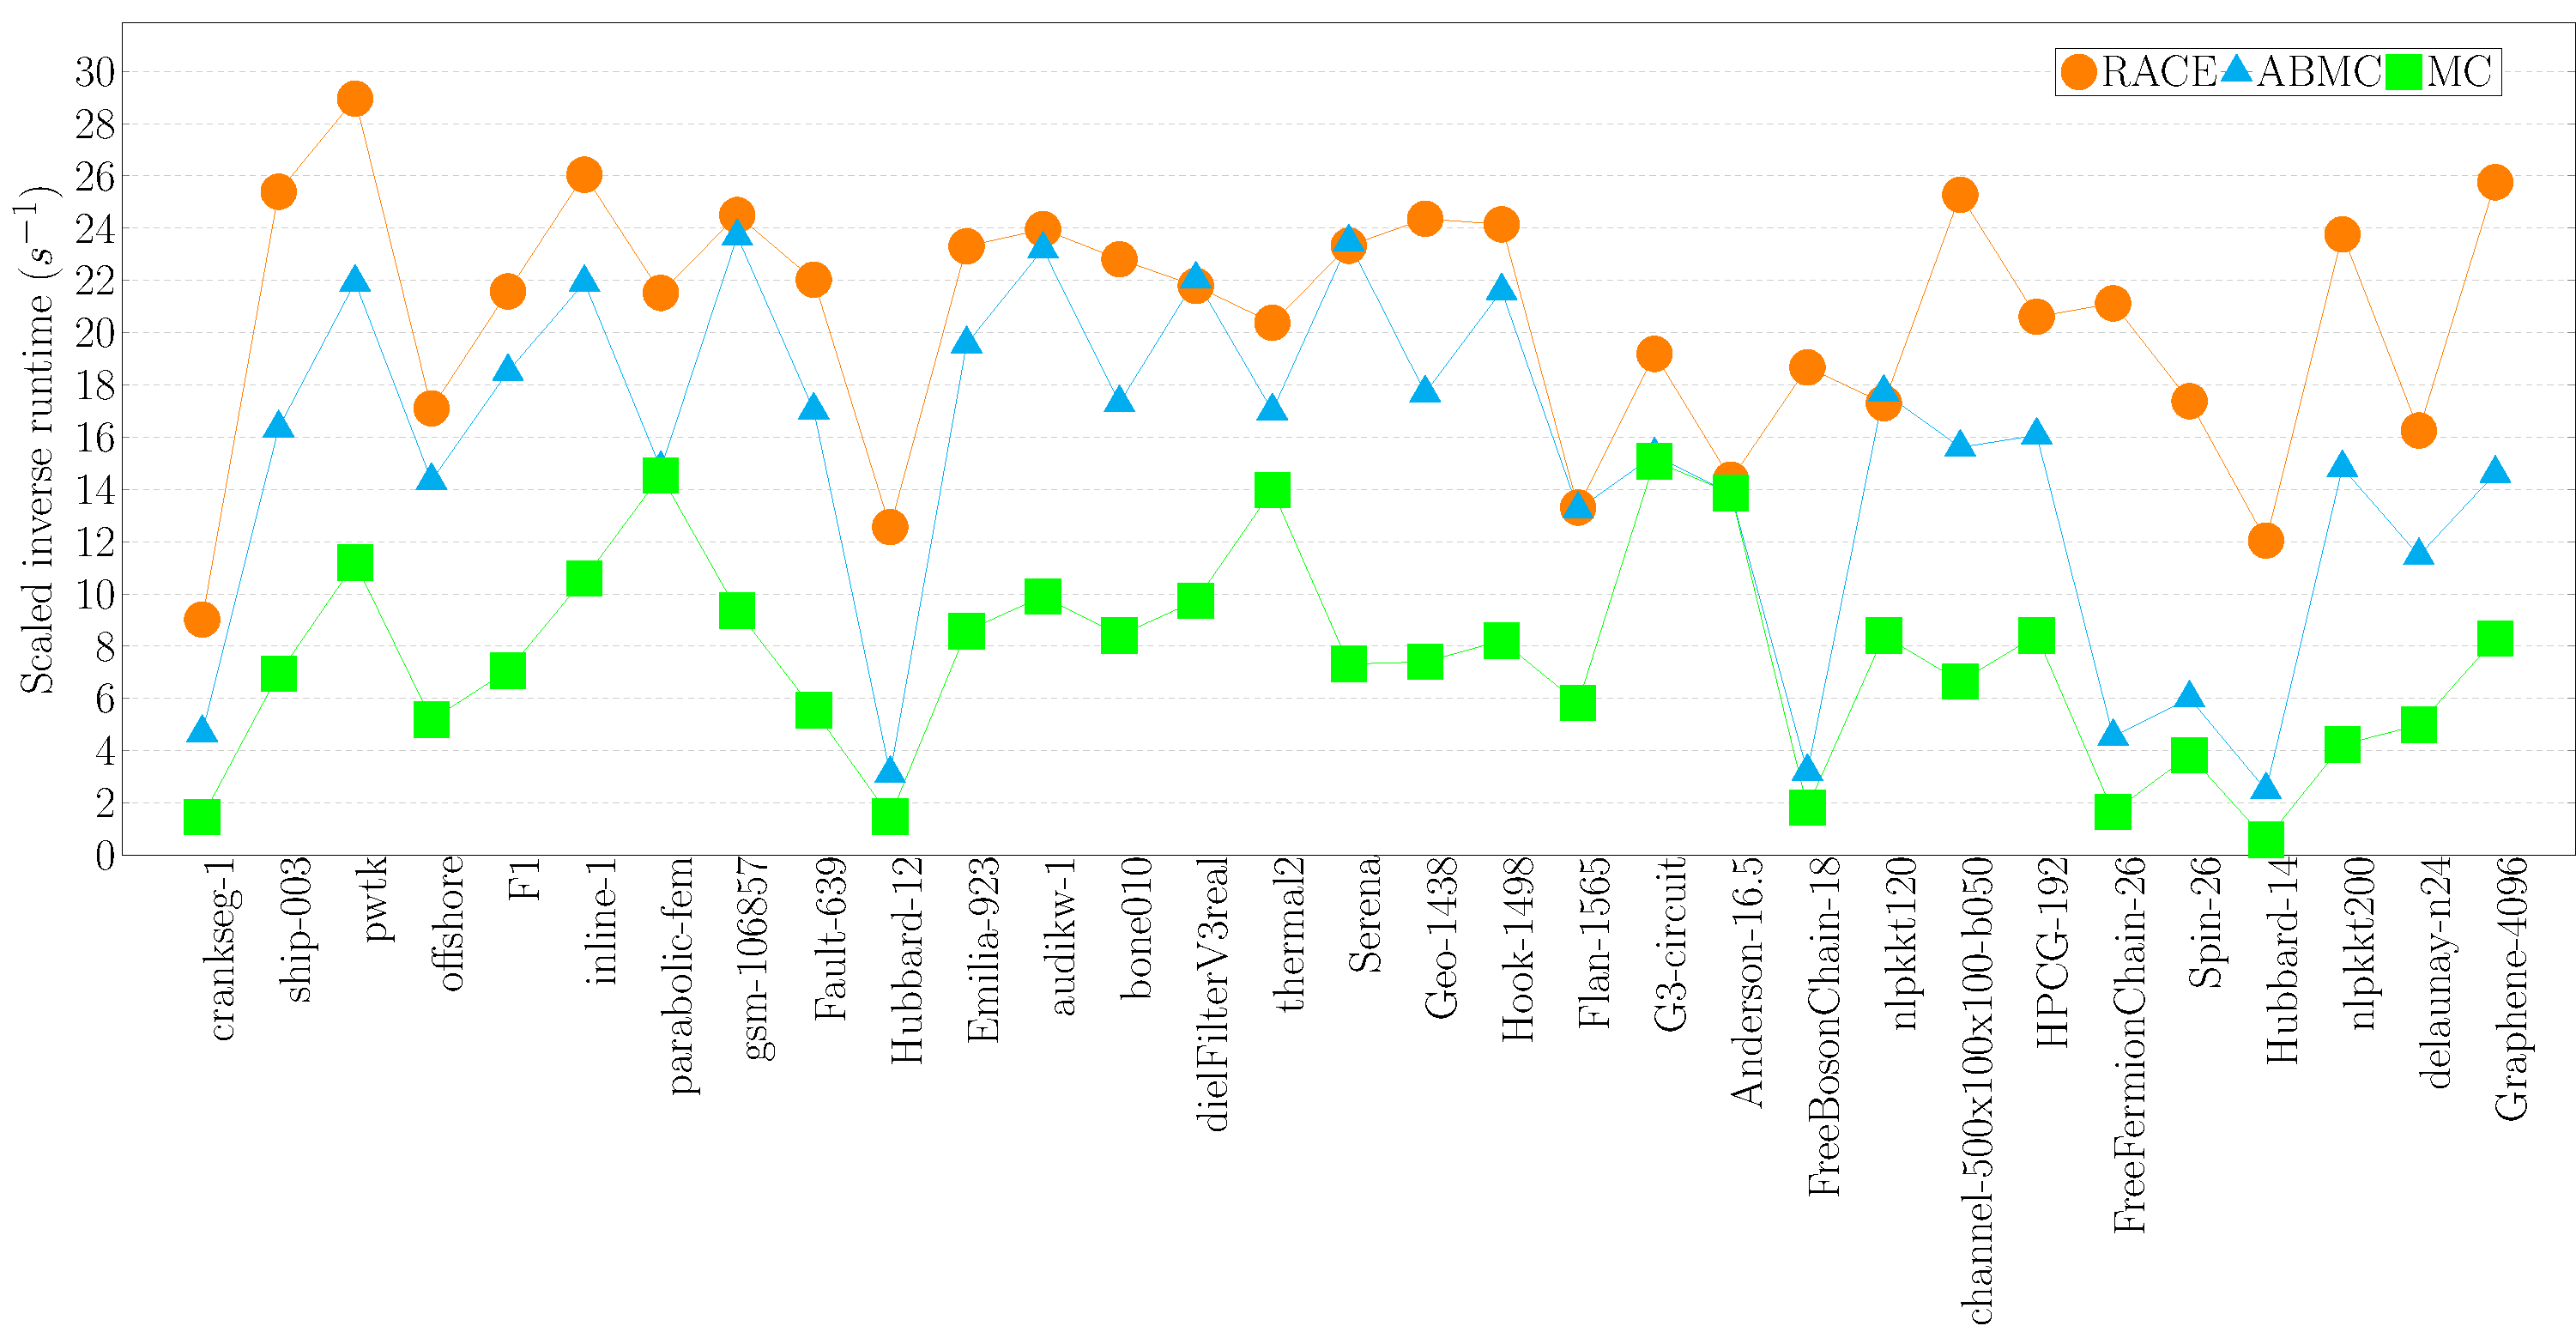
\includegraphics[width=0.85\textwidth, height=0.27\textheight]{pics/results/skx/data_symm_kacz/plot_generator/derived_perf_vs_mtx/derived_perf}}
	\caption{\SYMMKACZ inverse runtime (scaled)}
	\label{fig:symmkacz_dp}
\end{figure}

\begin{figure}[thbp]
	\centering
	\subfloat[Plain performance] {\label{fig:perf_kacz_ivb}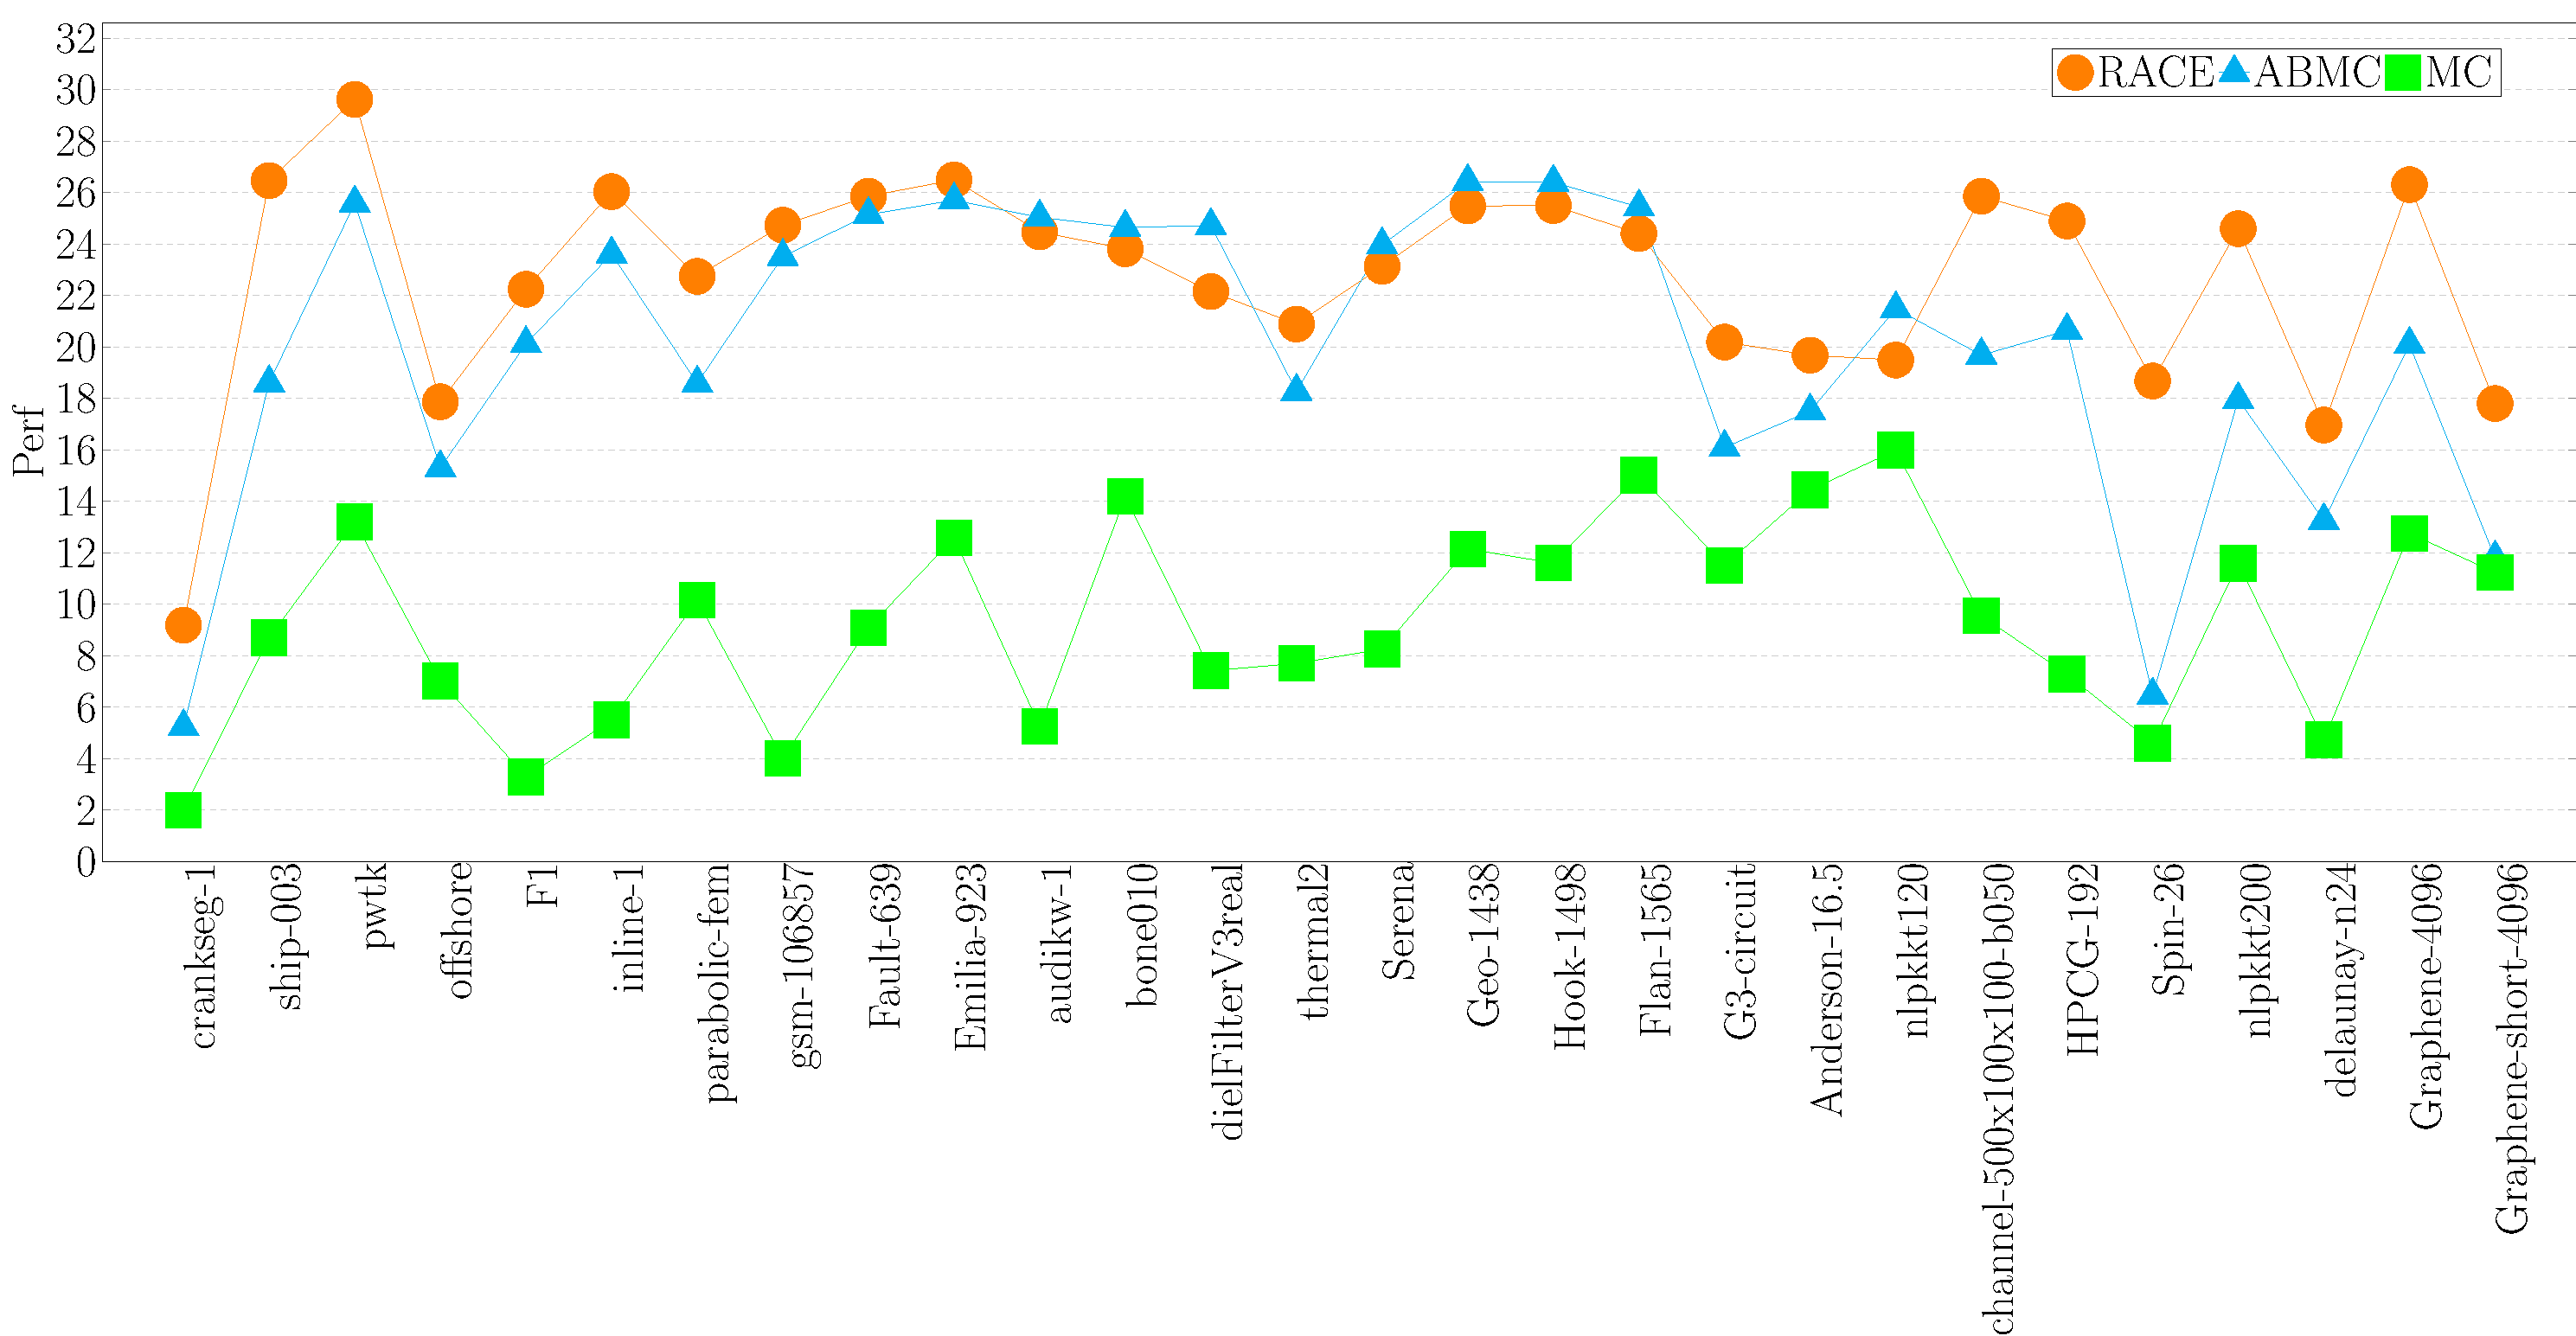
\includegraphics[width=0.85\textwidth, height=0.27\textheight]{pics/results/skx/data_symm_kacz/plot_generator/perf_vs_mtx/perf}}
	\hspace{1em}
	\subfloat[Iterations compared to serial Symm\KACZ kernel, note that for Hubbard-12, FreeBosonChain-18, FreeFermionChain-26 and Hubbard-14 the iteration count (y-axis) has to be multiplied by a factor of 50] {\label{fig:iter_kacz_skx}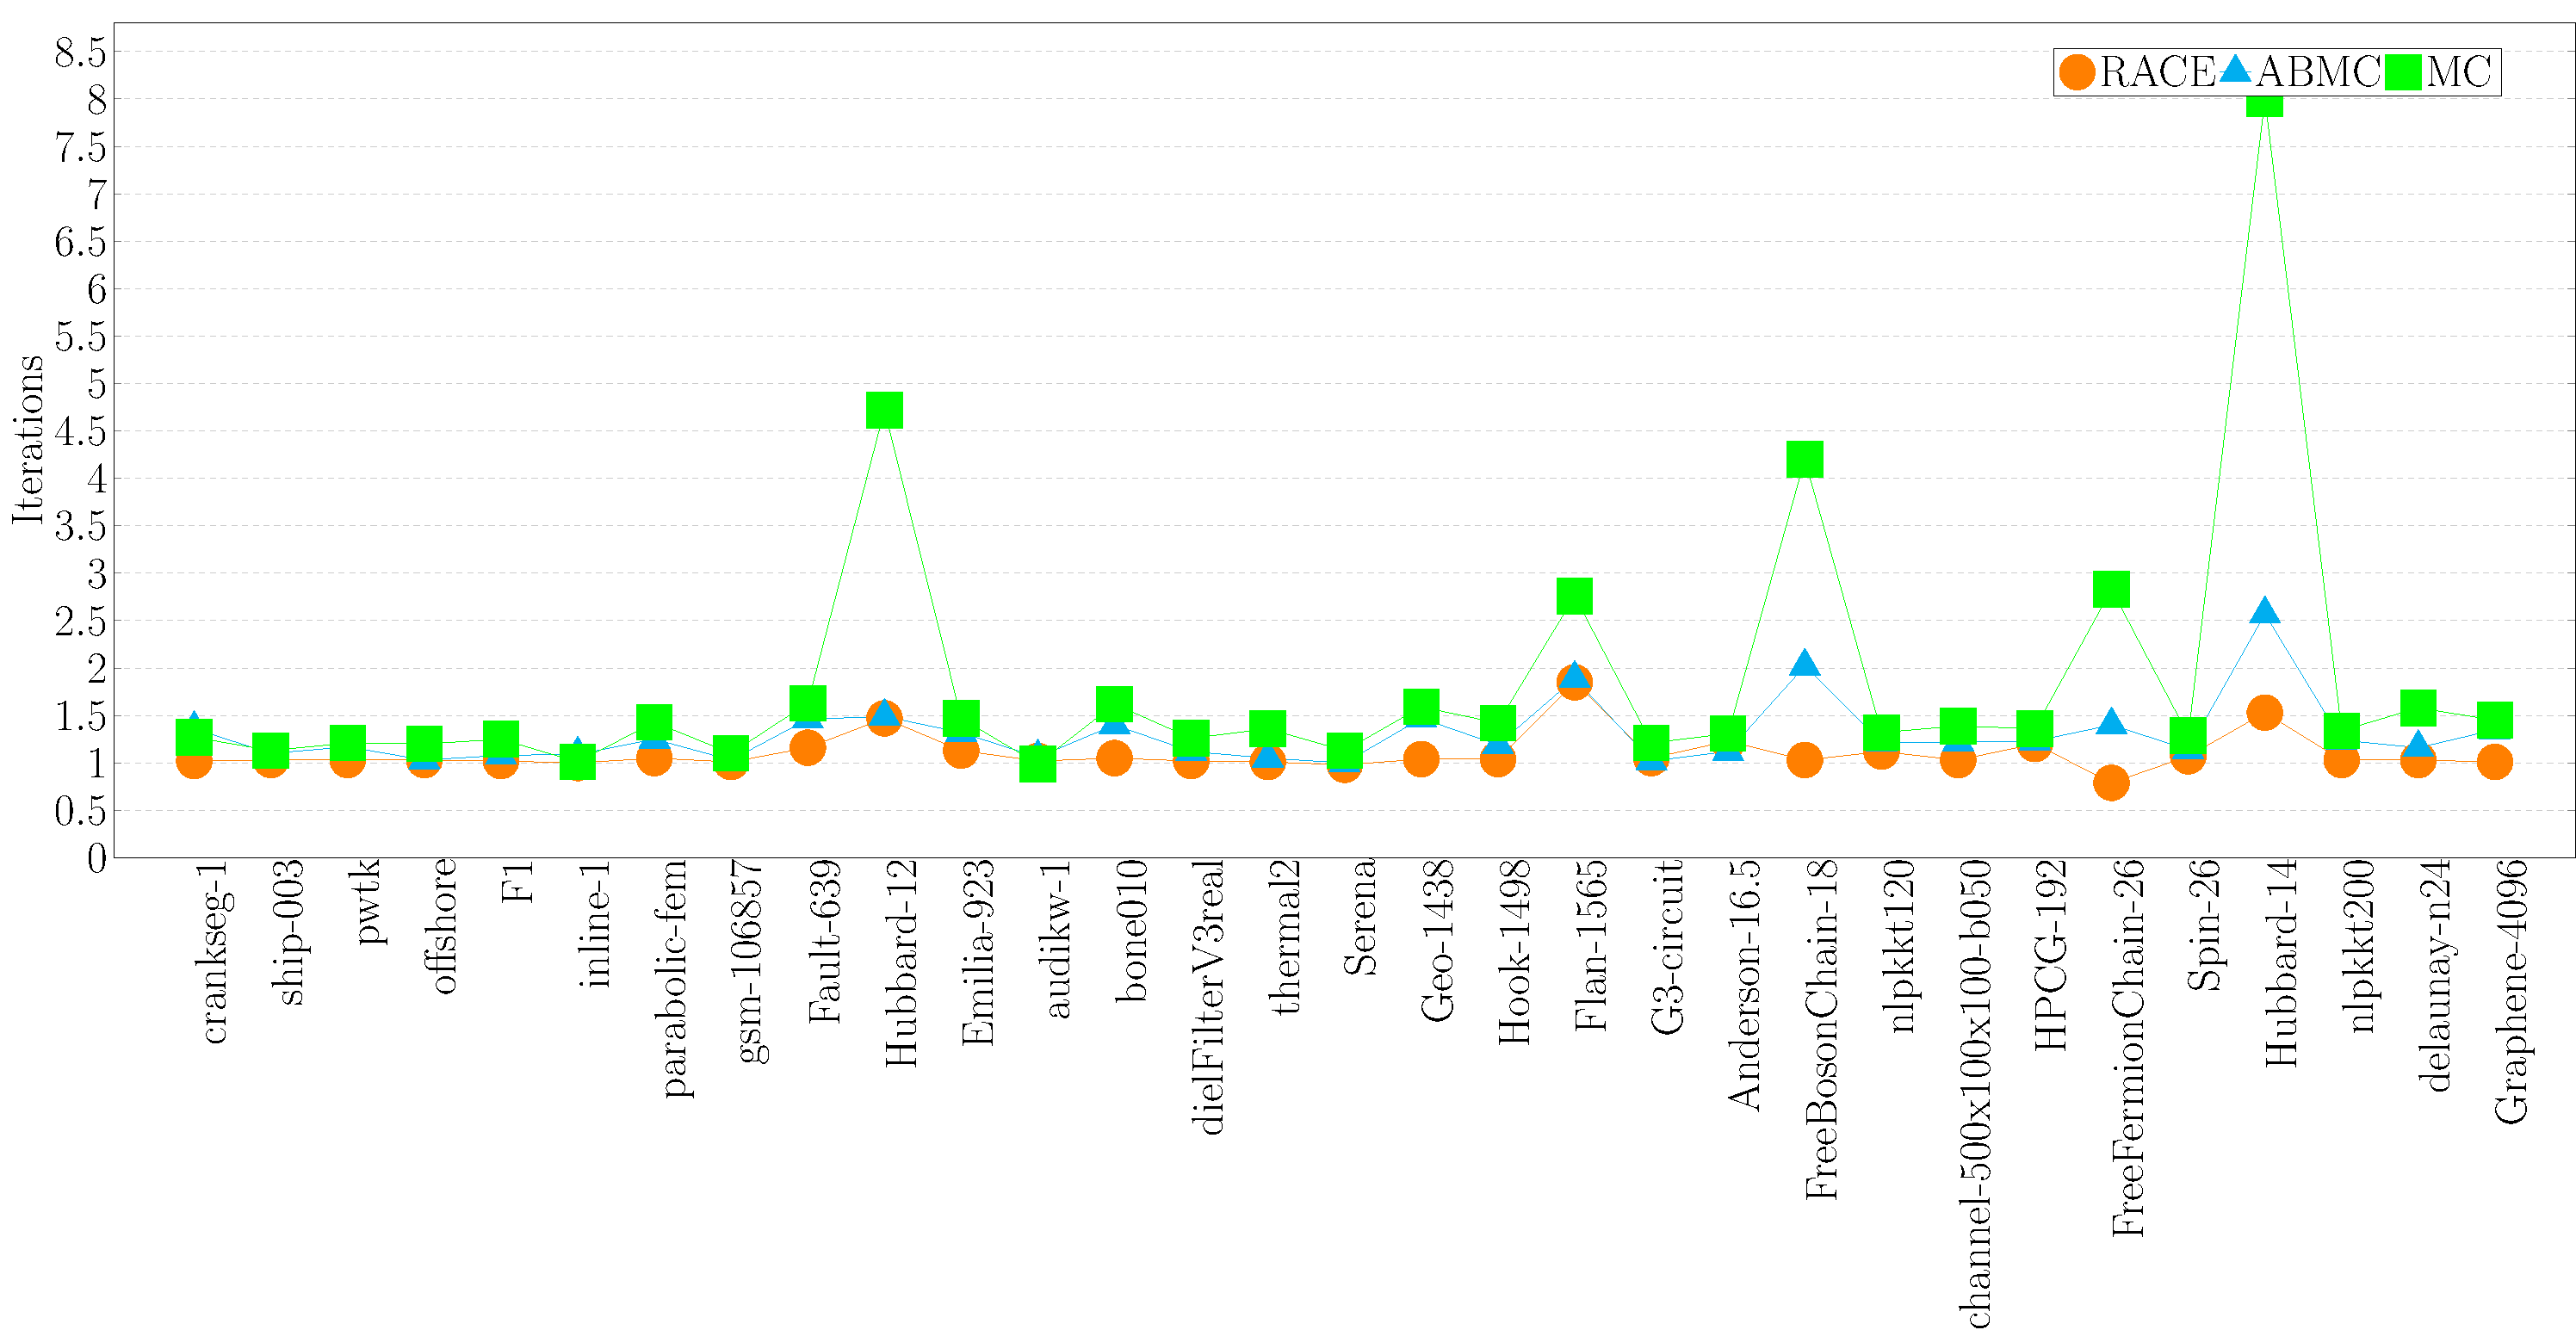
\includegraphics[width=0.85\textwidth, height=0.27\textheight]{pics/results/skx/data_symm_kacz/plot_generator/iter_vs_mtx/iter}}
	\caption{\SYMMKACZ convergence study on \SKX}
	\label{fig:symmkacz_convergence}
\end{figure}
\subsubsection{Iterative kernel}
Here we compare  \RACE with \ABMC and \MC for Symm\KACZ kernel. Inverse runtime of Symm\KACZ kernel is shown in \cref{fig:symmkacz_dp}.

 Since each of the matrix reordering changes convergence of the kernel, it is necessary here to also study the convergence behavior. \Cref{fig:symmkacz_convergence} shows the plain performance and iterations required on \SKX (20 threads) architecture.

Note that matrices only compatible with the \KACZ solvers are shown in performance results.

% The exact implementation of \MKL for \SYMMGS is not explicitly stated and is not published. But due to the property of the solver having same convergence as serial case we believe level-scheduling is used. The usage of same kernels in Intel's implementation of HPCG benchmark where the usage of level-scheduling has been stated \cite{Park_HPCG} leads to more confidence in our assumption.



\subsubsection{Comparison with tailored data format}
Comparison of \RACE with \RSB data format. Note \RSB is pre-processed with \RCM, which improves its performance for some cases. \Cref{fig:race_vs_rsb_ivy,fig:race_vs_rsb_skx} shows this comparison.

\begin{figure}[thbp]
	\centering
	\subfloat[Comparison of \RACE with \RSB on \IVB] {\label{fig:race_vs_rsb_ivy}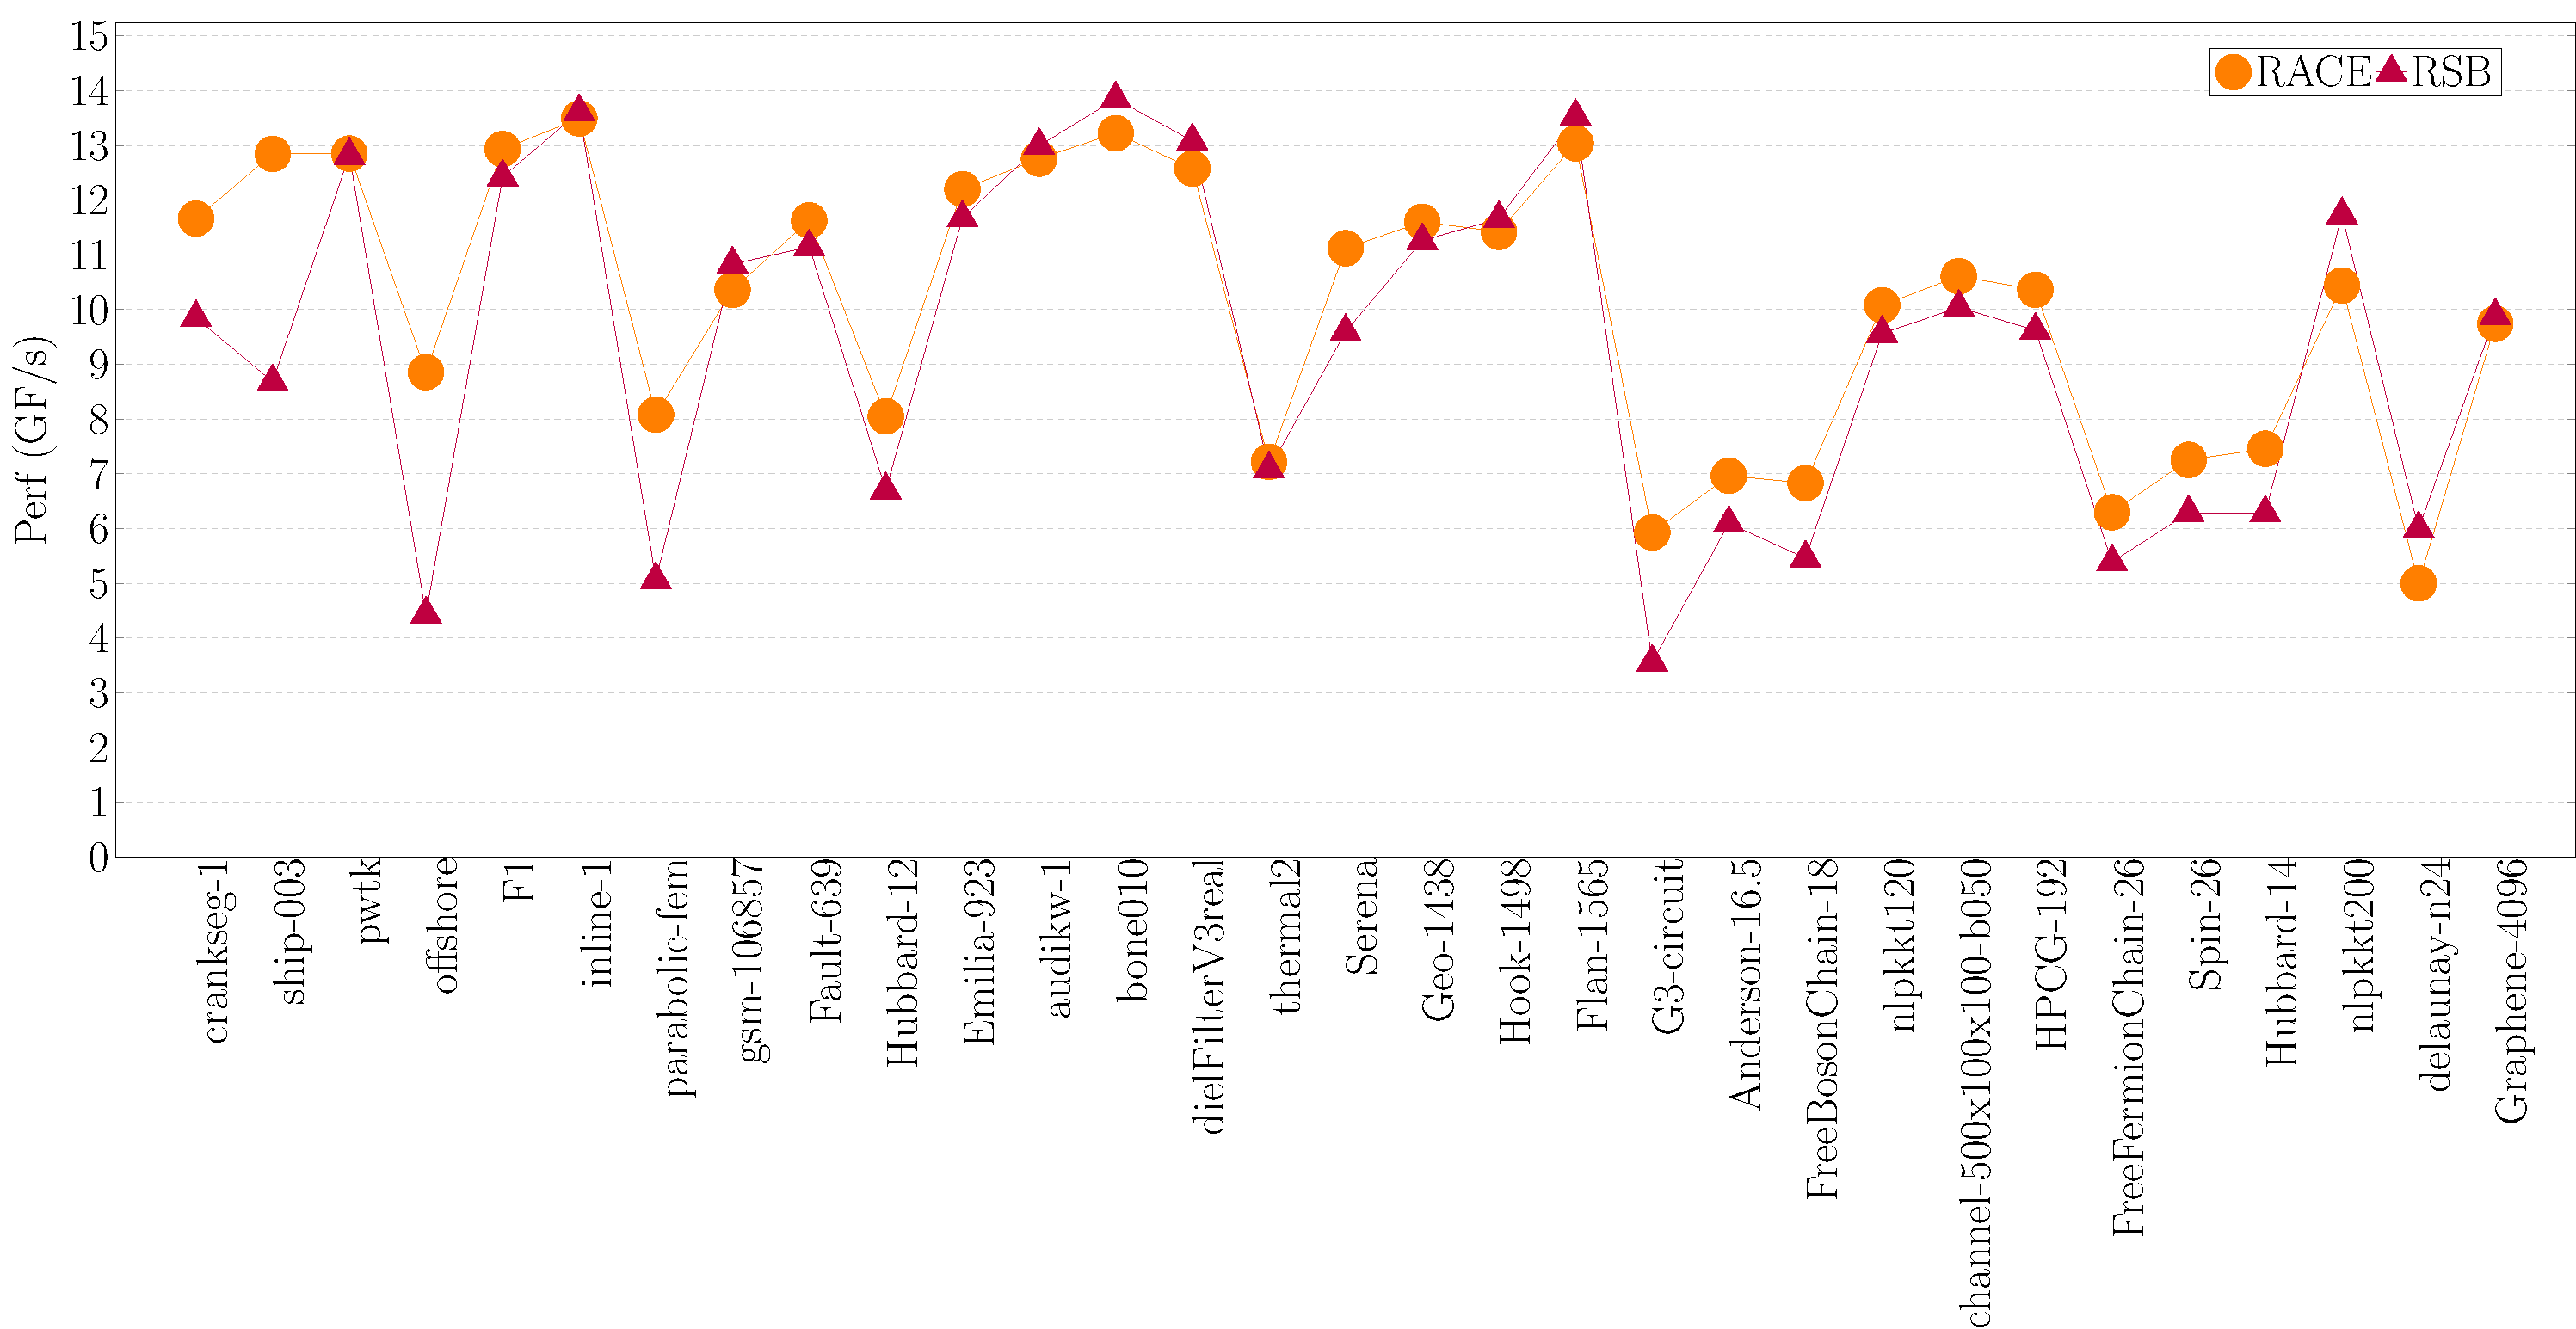
\includegraphics[width=0.45\textwidth, height=0.15\textheight]{pics/results/ivy/data_symm_spmv/plot_generator/perf_vs_mtx_w_RSB/perf}}
	\hspace{1.2em}
	\subfloat[Comparison of \RACE with \RSB on \SKX] {\label{fig:race_vs_rsb_skx}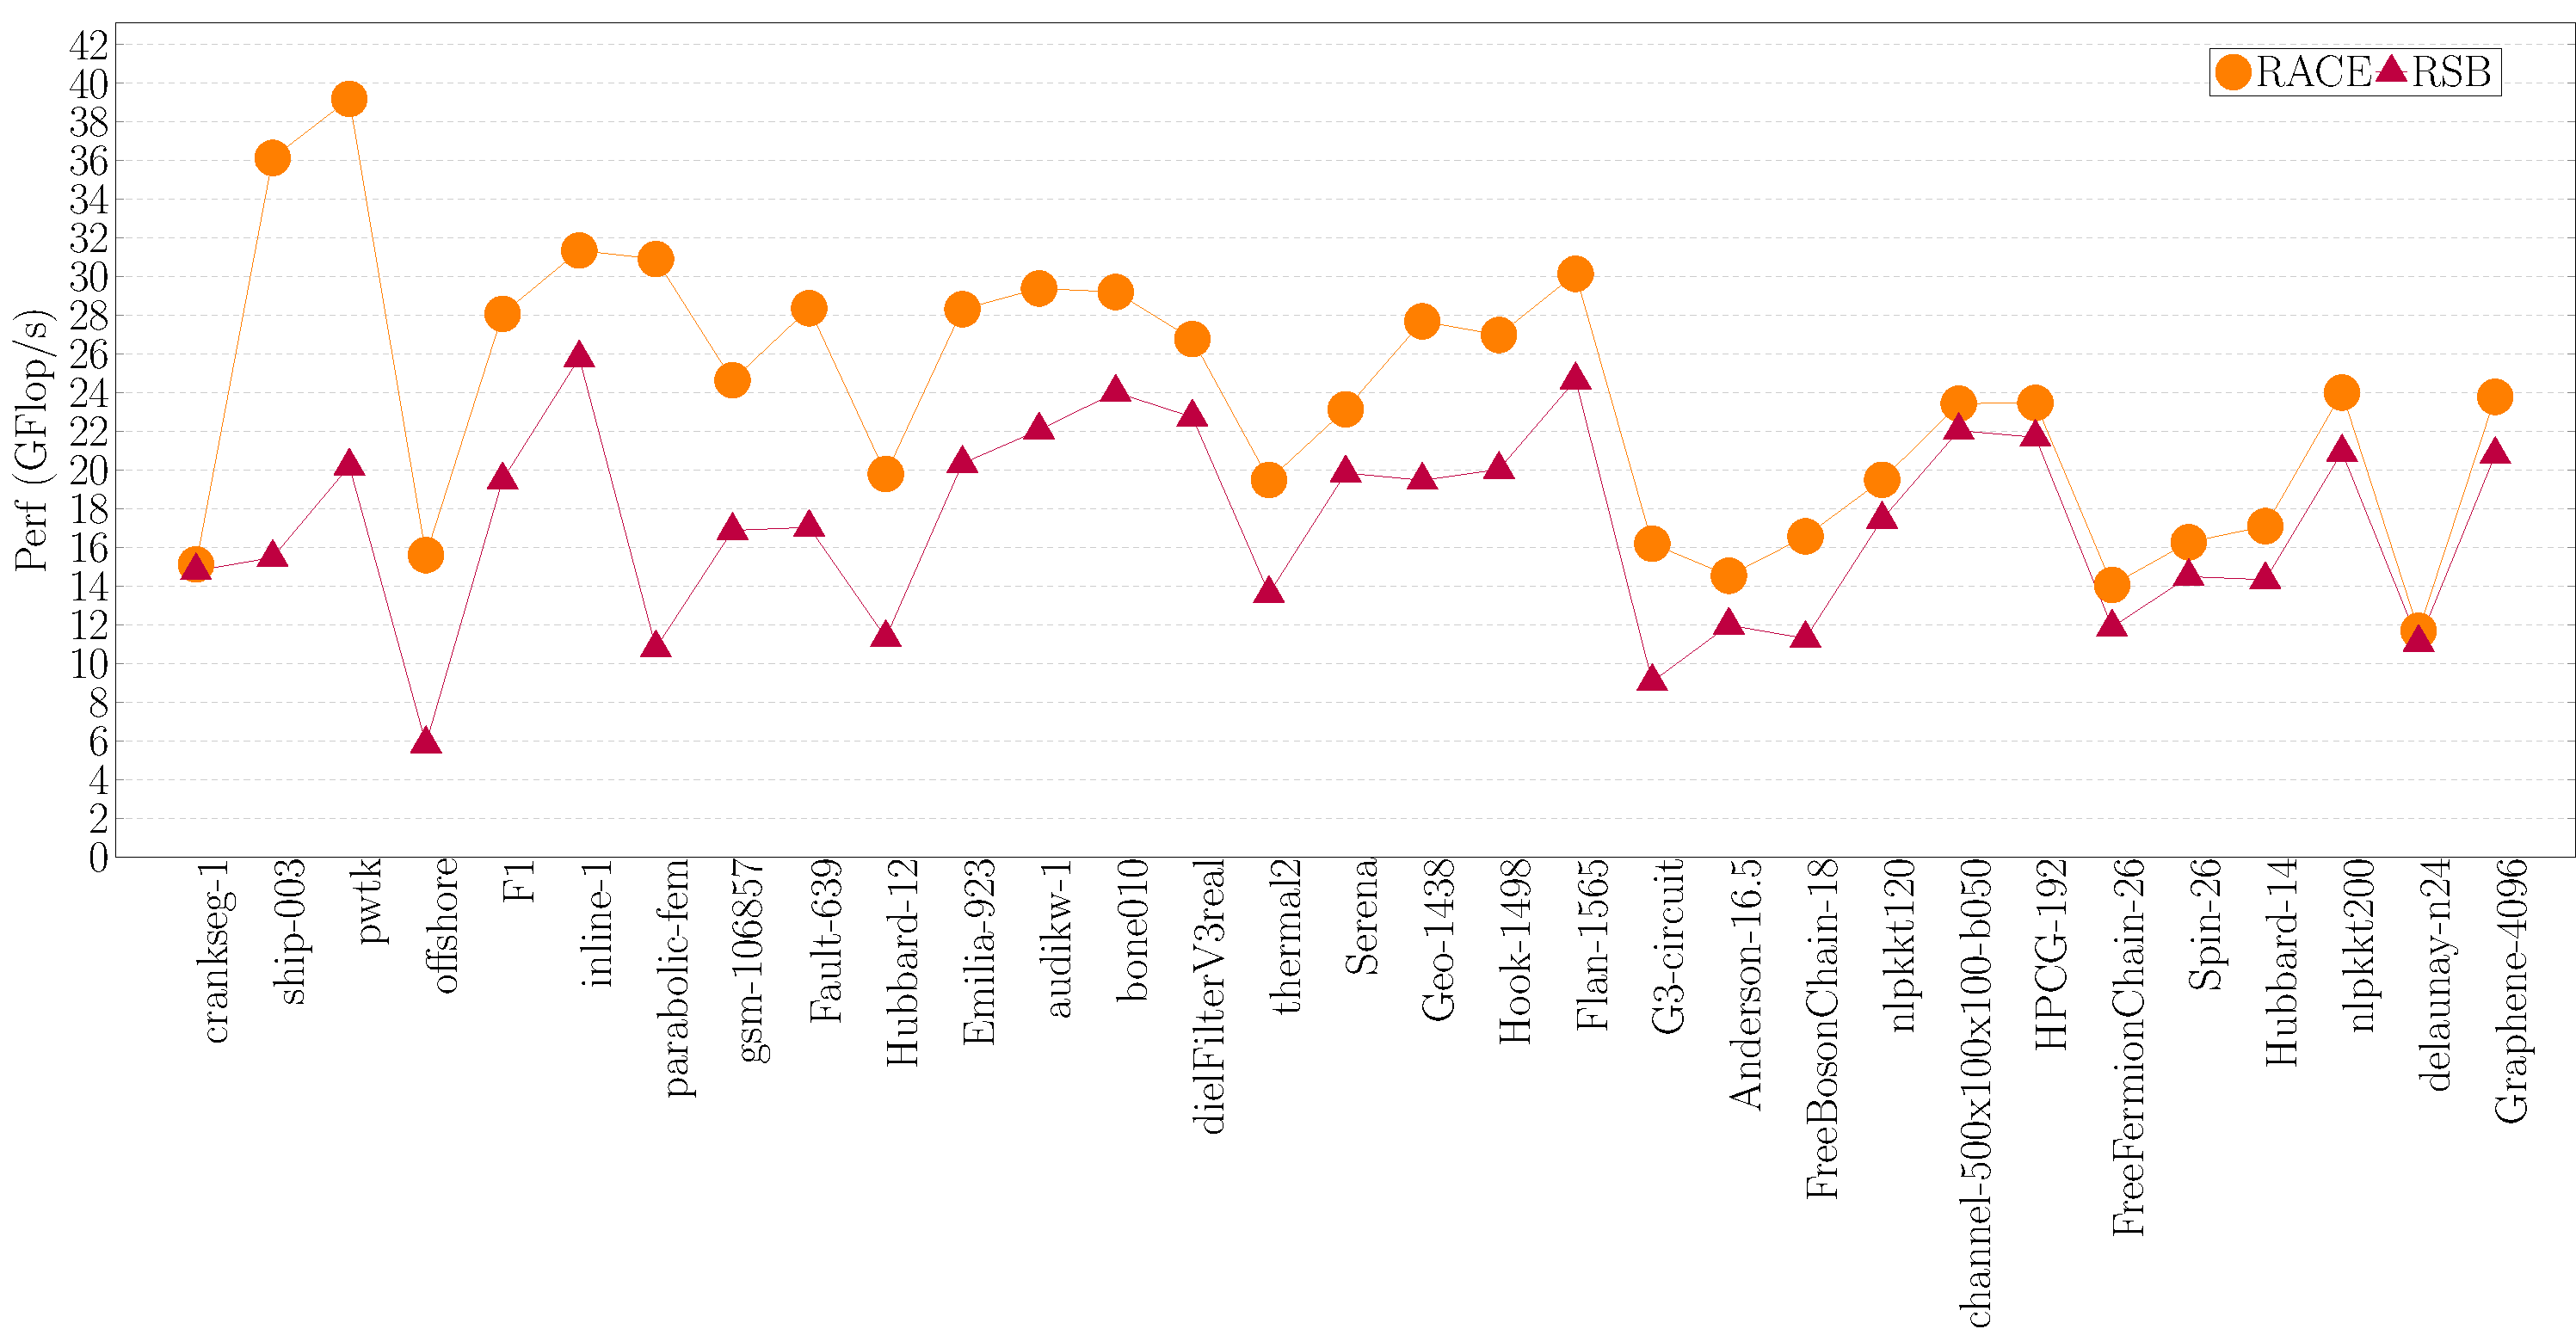
\includegraphics[width=0.45\textwidth, height=0.15\textheight]{pics/results/skx/data_symm_spmv/plot_generator/perf_vs_mtx_w_RSB/perf}}
	\caption{Comparison with \RSB data format}
	\label{fig:race_vs_rsb}
\end{figure}


\begin{comment}
\subsection{Main points to discuss}
\begin{itemize}
	\item Mention about specific setups like RCM for MKL and RSB, using IE for MKL
	\item Relate roofline model and the performance graphs of RACE compared to SpMV. 
	\item Point out on \IVB we reach close to ideal performance in every case, and on \SKX except for corner cases like crankseg and offshore we reach close to ideal performance. The drop in corner cases like crankseg and offshore on \SKX is due to lack of parallelism attained by RACE and associated load imbalances. This effect shows up on \SKX rather than \IVB since \SKX has 20 threads compared to 10 on \IVB.
	\item Point out that for cases like Graphene, Spin, parabolic\_fem we don't see 2 fold increase in GFlop/s for KACZ, and SymmSpMV. This is due to the fact here \NNZR is very small like 4, 14 and 7 which causes two problems. For KACZ kernel there is one division per row and this causes a performance drop as evident in Spin matrices, also this effect can be observed for GS kernel. For SymmSpMV kernel the \NNZR decreases almost by half since we operate only on upper triangular part and with short loop over \NNZR no effective vectorization and modulo unrolling can be done.
	\item Matrices like crankseg-1, and offshore are also really small making some part of data fit in cache, this is the reason why they achieve performance above RLM.
	\item Discuss why we chose the methods for comparison. MC and ABMC are common in literature for \DONE coloring, MKL methods are standard library used in many productive codes, also it uses level-scheduling (not explicitly stated but we believe) for kernels like GS and enables us to compare with methods that do not disturb convergence. RSB enables to compare with methods using different data format and it has been shown this method has an upper hand in this category. 
	\item Comparison with SymmSpMV shows the behavior of different methods for \DTWO coloring. Here we see in almost all of the case RACE and RSB has an upper hand on \IVB, although in some cases like offshore RACE clearly has an advantage. ABMC methods follow these methods. MKL and MC does not deliver good performance. For \SKX architecture \RSB falls behind \ABMC, we thing this is because of the requirement of \RSB to lock rows and cols of the submatrix on which a thread is working, becoming a bottleneck at high thread counts.
%	\item Explain SKX has slower stores, observable from load:copy benchmark ratio leading to SymmSpMV and KACZ not achieving two times SpMV, but on BDW this ratio is not much. This will get interesting with \EPY.
	\item Maybe tell RSB and 16-bit integer.
	\item Discuss with methods like ABMC and MC the performance especially drops for large matrices like Graphene, Spin, nlpkkt due to worsening of data locality ($\alpha$). Show sparsity pattern and \LIKWID meaurements. 
	\item Tell GS and KACZ performance includes also takes iterations into consideration (as shown in paper). Tell we do only a \DONE coloring for GS and \DTWO for KACZ. We use only matrices where GS can be applied and similarly for KACZ. Also we just compare against readily available solutions. Therefore RSB is left out for GS and RSB and MKL left out for KACZ.
	
\begin{figure}[thbp]
	\centering
	\subfloat[\SYMMGS iterations required by different methods compared to exact MKL kernel] {\label{fig:iter_gs}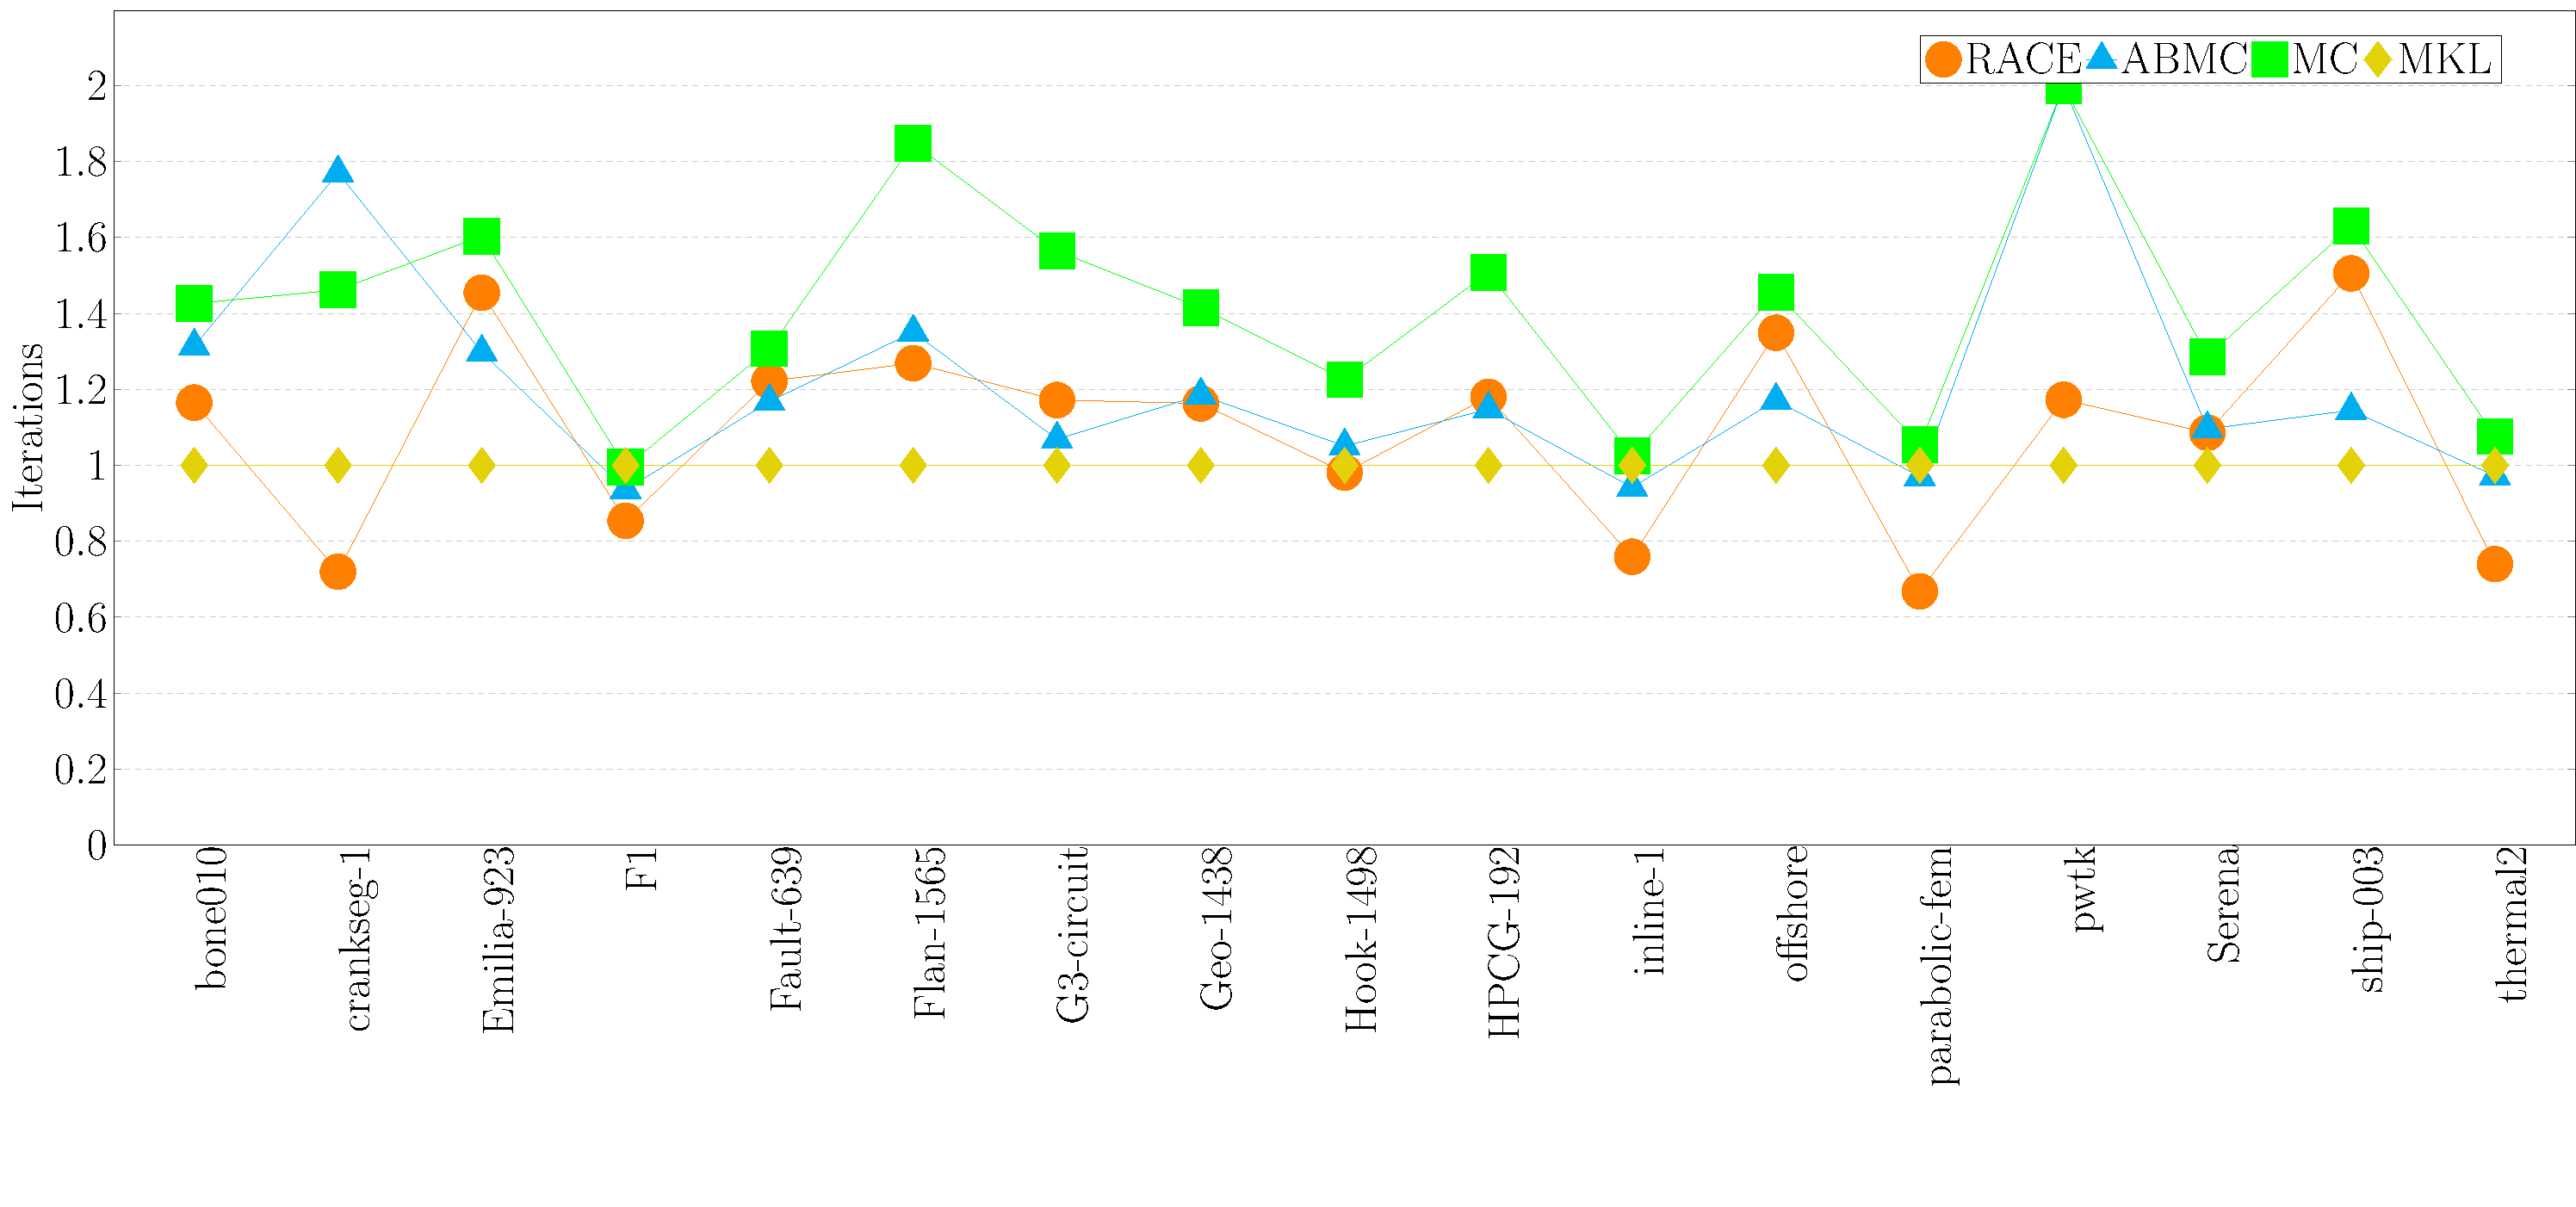
\includegraphics[width=0.49\textwidth, height=0.11\textheight]{pics/results/skx/iter/gs/plot}}
	\subfloat[\SYMMKACZ iterations required by different methods compared to exact Serial kernel] {\label{fig:iter_kacz}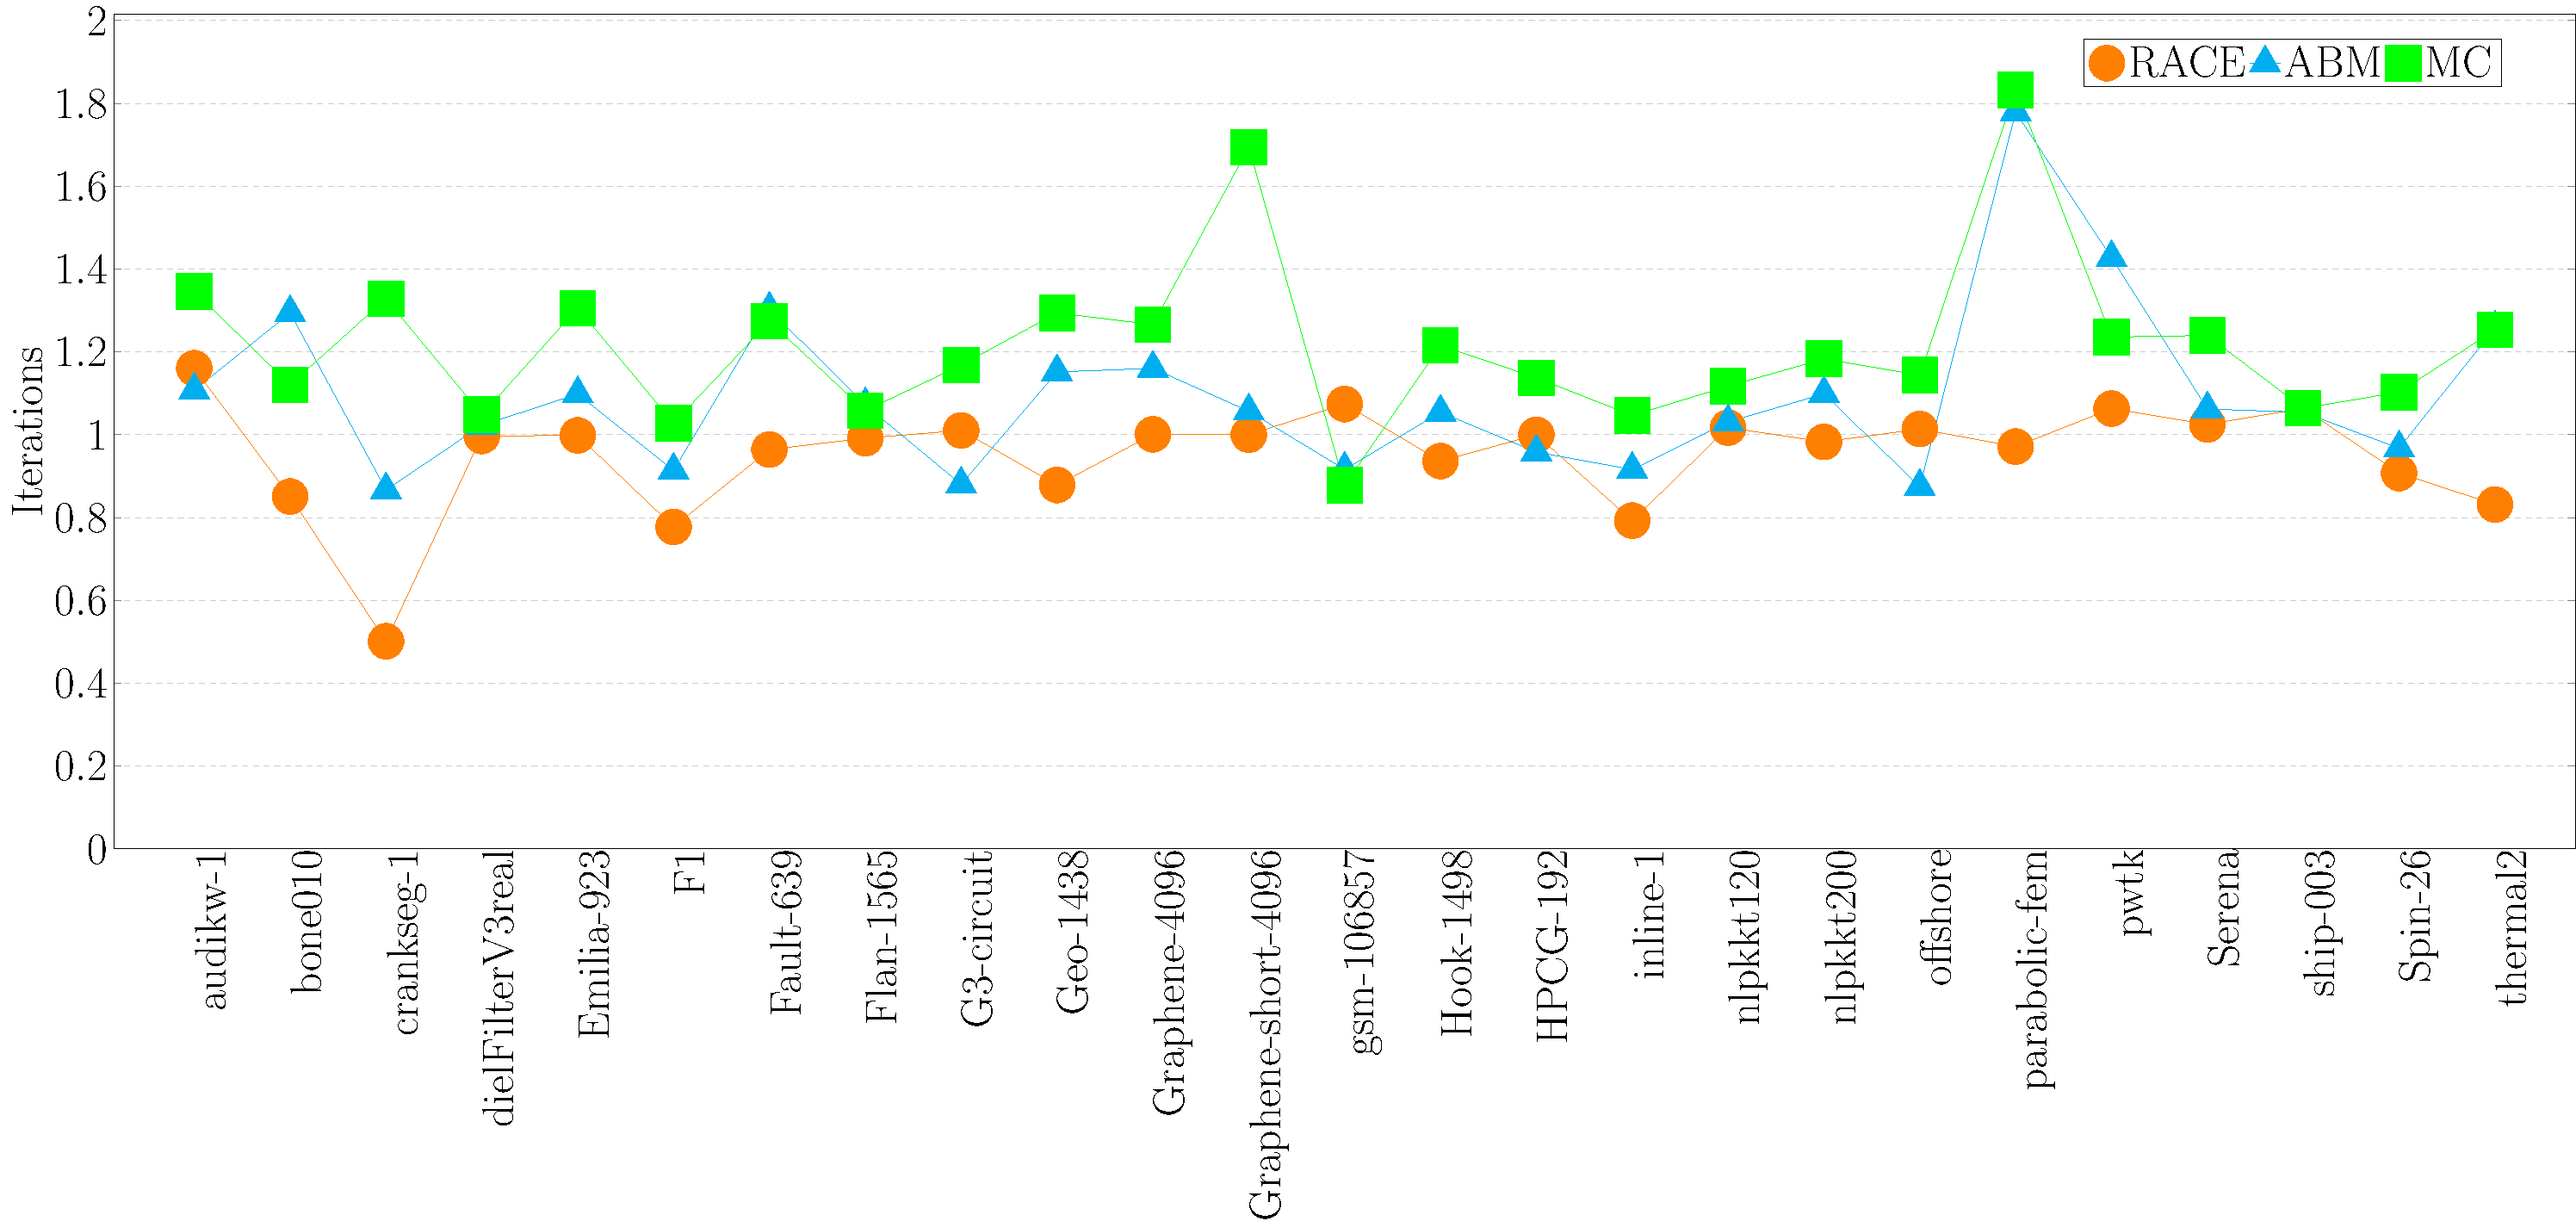
\includegraphics[width=0.49\textwidth, height=0.11\textheight]{pics/results/skx/iter/kacz/plot}}
	\caption{Convergence behavior of \SYMMGS and \SYMMKACZ at 20 threads}
	\label{fig:conv_behavior}
\end{figure}
	
	\item For GS RACE has an upper hand on \IVB and on \SKX RACE and ABMC have almost similar performance on \SKX, although for some cases RACE has huge advantage. Reason for this advantage is due to slight decrease in iterations for RACE (see \cref{fig:iter_gs}) and slight improvement in performance compared to ABMC for \DONE case. For offshore case RACE performs worser that ABMC, this is because here with RACE one requires more iterations. Also note that all the large matrices which we had are unsuitable for GS sweep as they do not converge, but for large matrices the performance drops again for ABMC method due to degrading of $\alpha$ factor. (Maybe just put perf. pictures).
	\item Main advantage of RACE method comes with kernels having \DTWO dependencies like SymmSpMV and KACZ since here methods like ABMC require more colors and their locality degrades further since here within a color rows have to be structurally orthogonal (rows shouldn't have common column entries). Performance on KACZ shows this advantage. Here we again see for moderately large matrices the advantage is higher. Iteration behavior between methods remains similar to GS (see \cref{fig:iter_kacz}).
\end{itemize}
 
\end{comment}
